% thesis.tex
%
% This file is root file for an example thesis written using the
% University of Wisconsin-Madison LaTeX Style file.
%
% It is provided without warranty on an AS IS basis.


%=====================================================================
% Document Style
%=====================================================================
% Choose only one of the following document classes:
%
% for a 12 Point UW PhD Thesis without Margin Check
%\documentclass[12pt, twosided]{withesis}
\documentclass[12pt,msthesis]{withesis}
%
% for a 10 Point UW PhD Thesis with Margin Check
%\documentclass[10pt,margincheck]{withesis}
%
% The margincheck option flags lines which overflow their hbox with a black
%  box at the end of the line.  This usually (but not always) indicates a
%  margin violation on the right margin.  Left margin violations aren't
%  indicated and if the margin violation is large enough, there isn't room
%  for the black box to be visiable.  
%
% This option can be also used in conjunction with the msthesis option.
%
% or for a 12 Point UW Masters Thesis
%\documentclass[12pt,msthesis]{withesis}
%
% or for a 10 Point UW Masters Thesis
%\documentclass[10pt,msthesis]{withesis}
%
% The msthesis option changes the page margins from 1" all around
% (the PhD format) to 1.25" left and 1" remaining margins (MS format).
% The defaults for degree and thesis are changed to be MS and thesis.
% These defaults can be overridden if the margins for the MS thesis
% are desired for other documents.

% To include optional packages, use the \usepackage command.
%  The package epsfig is used to bring in the Encapsulated PostScript
%    figures into the document.
%  The package times is used to change the fonts to Times Roman; however
%    because the times typewriter font looks odd, the original LaTeX
%    Computer Modern font is kept for the typewriter font using
%      \renewcommand{\ttdefault}{cmtt}
%    Note that Times Roman is a PostScript font and therefore, the document
%    cannot be correctly viewed from the *.dvi file.  It should be converted
%    to a *.ps file first and then viewed with a PostScript previewer...
\usepackage{epsfig}
\usepackage{times}
\renewcommand{\ttdefault}{cmtt}
\usepackage{amsmath}
\usepackage{graphicx} % for graphics files
\usepackage{subfigure} % for placing subfigures sids-by-side

% Draw figures yourself
\usepackage{tikz} 
\usepackage{fancyhdr} % used to put page number in header instead of footer

% The float package HAS to load before hyperref
\usepackage{float} % for psuedocode formatting
\usepackage{xspace}

% from Denovo Methods Manual
\usepackage{amssymb,amsthm}
\usepackage{mathrsfs}
\usepackage[mathcal]{euscript}
\usepackage{color}
\usepackage{array}
\usepackage{cite}
%\usepackage{c++}
%\usepackage{tmadd,tmath}
\usepackage{dsfont}

\usepackage[pdftex]{hyperref}

% define a style for pseudocode. This must load AFTER hyperref.
\floatstyle{ruled}
\newfloat{algorithm}{h}{lop}
\floatname{algorithm}{Algorithm}

%========================================================================
%  Draft Control Commands:
%========================================================================
%
% \psdraft causes the \psfig or \epsfig commands to draw a box and label
% the box with the postscript file name instead of reading in the full
% postscript figure.  This can save time and toner when printing drafts.
%
%\psdraft
%
%
% \psfull causes the inclusion of the postscript figures.
%\psfull
%
%
%\pagestyle{thesisdraft} causes the footer text to become:
% DRAFT: Do Not Distribute        <time><Date>        <input file name>
%
%\pagestyle{thesisdraft}
%
%\pagestyle{thesis} causes the header and footers to be the correct format
%
\pagestyle{thesis}
%
%
%  The page margins can be marked with a post-script box using the
%  \draftmargins command.  This command uses dvips's end-of-page hook
%  This is only visible in the *.ps file (NOT the *.dvi file)!
%
\draftmargins
%
%
%  The word ``DRAFT'' can be diagonally printed across the page using
%  the \draftscreen command.  This command uses dvip's beginning-of-page
%  hook.  This is only visible in the *.ps file (NOT the *.dvi file)!
%
%\draftscreen


%=======================================================================
% Remove the following lines if appendix tables or figures are present.
% The suppress writing the auxiliary information which appears in the
% list of tables or list of figures.
%
\noappendixtables                % Don't have appendix tables
\noappendixfigures               % Don't have appendix figures
%\noappendixalgorithms         % Don't have appendix algorithms

\newcommand{\Macro}{\ensuremath{\Sigma}}

\newcommand{\Sn}{\ensuremath{S_N} }
\newcommand{\vOmega}{\ensuremath{\hat{\Omega}}}
\newcommand{\Ye}[2]{\ensuremath{Y^e_{#1}(\vOmega_#2)}}
\newcommand{\Yo}[2]{\ensuremath{Y^o_{#1}(\vOmega_#2)}}

\newcommand{\ve}[1]{\ensuremath{\mathbf{#1}}}

\newcommand{\sigg}[1]{\ensuremath{\Macro^{gg'}_{s\,#1}}}
\newcommand{\psig}{\ensuremath{\psi^g}}

\newcommand{\even}{\ensuremath{\phi^g}}
\newcommand{\odd}{\ensuremath{\vartheta^g}}
\newcommand{\evenp}{\ensuremath{\phi^{g'}}}
\newcommand{\oddp}{\ensuremath{\vartheta^{g'}}}

\newcommand{\mg}{multigrid }
%=======================================================================
% End of Preamble, start of document
%
\begin{document}

% Choose your bibliography style
% plain is the basic style, others include ieee, siam, asm, etc
\bibliographystyle{plain}

 % prelude.tex
%   - titlepage
%   - acknowledgments
%   - table of contents, list of tables and list of figures
%   - umiabstract
%   - abstract
%============================================================================


\clearpage\pagenumbering{roman}  % This makes the page numbers Roman (i, ii, etc)



% TITLE PAGE
%   - define \title{} \author{} \date{}
\title{ACCELERATION METHODS FOR MASSIVELY PARALLEL DETERMINISTIC TRANSPORT}
\author{Rachel N. Slaybaugh}
\date{\today}
%   - The default degree is ``Doctor of Philosophy''
%     (unless the document style msthesis is specified
%      and then the default degree is ``Master of Science'')
%     Degree can be changed using the command \degree{}
\degree{Doctor of Philosophy}
%   - The default is dissertation, unless the document style
%     msthesis was specified in which case it becomes thesis.
%     If msthesis is specified for the MS margins, you can
%     still have a dissertation if you specify \disseration
%\disseration
%   - for a masters project report, specify \project
%\project
%   - for a preliminary report, specify \prelim
%\prelim
%   - for a masters thesis, specify \thesis
\thesis
%   - The default department is ``Electrical Engineering''
%     The department can be changed using the command \department{}
%\department{New Department}
%   - once the above are defined, use \maketitle to generate the titlepage
\department{Engineering Physics}
\maketitle

% COPYRIGHT PAGE
%   - To include a copyright page use \copyrightpage
\copyrightpage

% DEDICATION
%\begin{dedication}
%To my pet rock, Skippy.
%\end{dedication}

% ACKNOWLEDGMENTS
\begin{acknowledgments}
First and foremost I would like to thank my thesis advisor Paul Wilson, my project mentor Tom Evans, and my fellowship mentor Tom Sutton for their instruction and guidance. I would also like to thank Steve Wilson, my mentor from my summer practicum at Bettis. Many individuals such as Yousry Azmy and Bernadette Kirk, among others, have been instrumental to my professional development as well. Greg Davidson was extremely helpful throughout my work on Denovo. It was wonderful to work with my colleagues at Karlsruhe. Milad Fatenejad and Katy Huff made my life easier by teaching me about software carpentry while feeding me brownies and making me laugh. I'd also like to thank the department for making me a better runner. 

This research was performed under appointment to the Rickover Fellowship Program in Nuclear Engineering sponsored by Naval Reactors Division of the U.S.\ Department of Energy. I would also like to thank Oak Ridge National Laboratory and their computing facilities (OLCF) for computer time and project support. 

Finally, I would like to thank my friends and family, without whom I could not do much of anything. My mom has always been my hero; my Dad is good at telling me he's proud of me; I've had fun watching my brother become a rock star in his own right;  Sam, Jenna, and David have long served as confidants; Julie and Megan have kept me laughing since I met them; all of my roommates in grad school have put up with my crazy kitchen adventures; the hash has kept me running; and all the folks I love who I haven't called out individually have kept things interesting. Thank you all for inspiring me and making my life fun, fulfilling, and wonderful.

\end{acknowledgments}

% CONTENTS, TABLES, FIGURES
\tableofcontents
\listoftables
\listoffigures
%\listof{table}{LIST OF TABLES}
%\listof{figure}{LIST OF FIGURES}
%\listofalgorithms
%\listof{algorithm}{LIST OF ALGORITHMS}

% NOMENCLATURE
%\begin{nomenclature}
%\begin{description}
%\item{\makebox[0.75in][l]{\TeX}}
%       \parbox[t]{5in}{a typesetting system by Donald Knuth~\cite{knuth}.  It
%       also refers to the ``plain'' format.  The proper pronounciation
%       rhymes with ``heck'' and ``peck'' and does not sound like
%       ``hex'' or ``Rex.''\\}

%\item{\makebox[0.75in][l]{\LaTeX}}  
%        \parbox[t]{5in}{a set of \TeX{} macros originally written by Leslie 
%        Lamport~\cite{lamport}.  The proper pronunciation is 
%        {\tt l\={a}$\cdot$tek'} and not {\tt l\={a}'$\cdot$teks} (see above).\\}

%\item{\makebox[0.75in][l]{{\sc Bib}\TeX}} 
%         \parbox[t]{5in}{a bibliography generation program by Oren 
%                Patashnik~\cite{lamport}
%                that can be used with either plain \TeX{} or \LaTeX{}.\\}

%\item{\makebox[0.75in][l]{$C_1$}} Constant 1

%\item{\makebox[0.75in][l]{$V$}}    Voltage 

%\item{\makebox[0.75in][l]{\$}}     US Dollars
%\end{description}
%\end{nomenclature}


%\advisorname{Paul P. H. Wilson}
%\advisortitle{Associate Professor}
%% ABSTRACT
%\begin{umiabstract}
%  % Thesis, Absatract
% by Rachel Slaybaugh

\noindent       % Don't indent this paragraph.
To improve the design of nuclear systems, high-fidelity neutron fluxes are required. Leadership-class machines provide platforms on which very large problems can be solved. Computing such fluxes efficiently requires numerical methods with good convergence properties and algorithms that can scale to hundreds of thousands of cores. Many 3-D deterministic transport codes are decomposable in space and angle only, limiting them to tens of thousands of cores. Most codes rely on methods such as Gauss Seidel for fixed source problems and power iteration for eigenvalue problems, which can be slow to converge for challenging problems like those with highly scattering materials or high dominance ratios. 

\vspace*{0.5em}
\noindent       % Don't indent this paragraph.
Three methods have been added to the 3-D \Sn transport code Denovo that are designed to improve convergence and enable the full use of cutting-edge computers. The first is a multigroup Krylov solver that converges more quickly than Gauss Seidel and parallelizes the code in energy such that Denovo can use hundreds of thousand of cores effectively. 

\vspace*{0.5em}
\noindent       % Don't indent this paragraph.
The second is Rayleigh quotient iteration (RQI), an old method applied in a new context. This eigenvalue solver finds the dominant eigenvalue in a mathematically optimal way and should converge in fewer iterations than power iteration. RQI creates energy-block-dense equations that the new Krylov solver treats efficiently. However, RQI can have convergence problems because it creates poorly conditioned systems. This can be overcome with preconditioning. 

\vspace*{0.5em}
\noindent       % Don't indent this paragraph.
The third method is a multigrid in energy preconditioner. The preconditioner takes advantage of the new energy decomposition because the grids are in energy rather than space or angle. The preconditioner greatly reduces iteration count for many problem types and scales well in energy. It also allows RQI to be successful for problems it could not solve otherwise. 

\vspace*{0.5em}
\noindent       % Don't indent this paragraph.
The methods added to Denovo accomplish the goals of this work. They converge in fewer iterations than traditional methods and enable the use of hundreds of thousands of cores. Each method can be used individually, with the multigroup Krylov solver and multigrid-in-energy preconditioner being particularly successful on their own. The largest benefit, though, comes from using these methods in concert. 

%\end{umiabstract}

\begin{abstract}
  % Thesis, Absatract
% by Rachel Slaybaugh

\noindent       % Don't indent this paragraph.
To enhance and improve the design of nuclear systems, high-fidelity neutron fluxes are required. For today's problems, high-fidelity means thousands $\times$ thousands $\times$ thousands of mesh points, up to $\sim$150 energy groups, accurate scattering expansions, and the use of many directions. Leadership-class machines provide platforms on which problems of this size can be solved in a reasonable amount of time. Computing such fluxes accurately and efficiently requires numerical methods with good convergence properties and algorithms that can scale to hundreds of thousands of cores. 

\vspace*{0.5em}
\noindent       % Don't indent this paragraph.
Many 3-D deterministic transport codes can scale in space and angle to tens of thousands of cores. They typically rely on methods such as Gauss Seidel for fixed source problems and power iteration for eigenvalue problems. Within group solvers range from source iteration to Krylov methods. In many cases these methods are accelerated with strategies like coarse mesh rebalance, diffusion synthetic acceleration, and others. Nevertheless, these problems can be slow to converge for challenging problems like those with highly scattering materials or high dominance ratios. 

\vspace*{0.5em}
\noindent       % Don't indent this paragraph.
Three methods have been added to Denovo, a 3-D \Sn transport code, that are designed to improve convergence and enable the full use of cutting-edge computers. The first method added was a multigroup Krylov solver that improves convergence when compared to Gauss Seidel and dramatically increases the number cores Denovo can use. Tests show that the multigroup Krylov solver can substantially outperform Gauss Seidel in challenging problems. The energy decomposition added by the solver allowed Denovo to solve problems on 100,000 and 200,000 cores. 

\vspace*{0.5em}
\noindent       % Don't indent this paragraph.
The second method is Rayleigh quotient iteration (RQI), an old method being applied in a new context. This eigenvalue solver finds the dominant eigenvalue in an optimal way, and theory indicates that RQI should converge in fewer iterations than traditional eigenvalue solvers. RQI creates an energy-block dense system that would be difficult for Gauss Seidel. The new Krylov solver treats this kind of system very efficiently, and RQI would not be a good choice without it. Unfortunately, RQI also creates poorly conditioned systems such that the method is only useful in very simple problems. However, preconditioning can alleviate this problem. 

\vspace*{0.5em}
\noindent       % Don't indent this paragraph.
The final method is a multigrid in energy, physics-based preconditioner. The selection of using grids in energy rather than space or angle means the preconditioner can easily take advantage of energy parallelization. Further, the convergence behavior of the Krylov iterations inside RQI looks like the type of problem for which multigrid methods are most useful. The new preconditioner was very effective at reducing multigroup iteration count for many types of problems. In some cases it also reduced eigenvalue iteration count. The preconditioner scaled very well in energy, and was tested on up to 200,000 cores on a full-facility PWR.

\vspace*{0.5em}
\noindent       % Don't indent this paragraph.
When RQI was preconditioned with multigrid in energy it was able to solve nearly all test problems in a small number of iterations. The preconditioned RQI calculations also scaled well in energy. For large, challenging problems RQI was also much faster than power iteration. Some more punchline-type statements.

\vspace*{0.5em}
\noindent       % Don't indent this paragraph.
Some summarizing paragraph wrapping everything up. 



\end{abstract}


\clearpage\pagenumbering{arabic} % This makes the page numbers Arabic (1, 2, etc)

\separatorpage{}
           % Title page, abstract, table of contents, etc
 %Prelim, Chapter 1
% by Rachel Slaybaugh

\chapter{Introduction}
\label{sec:Chp1}

Nuclear technology plays an important role in society, particularly within the field of energy generation. More nuclear reactors are being constructed, existing designs are being refined, and new plants are being developed. For progress to continue in these areas, the modeling of nuclear systems must also progress. 

The neutron transport equation describes ``where all the neutrons are'' in a nuclear system. The more accurately this is known, the more accurately new systems can be developed. This means that solutions to the transport equation are needed in high-fidelity in all parts of phase space. Very large computers are now available to perform such high-fidelity calculations, but most existing solution methods are not able to take full advantage of new computer architectures. This work aims to accelerate the transport solution with new methods that use new machines fully, facilitating the design of better nuclear systems. 

The goal of this research is to accelerate transport calculations with methods that use new computers fully, facilitating the design of better nuclear systems. Three complimentary methods have been implemented to accomplish this goal. In the chapters that follow this, background information, past work, mathematics and implementation, and results will be discussed for each method in turn. 

This introductory chapter is intended to provide the foundation of this document. The types of problems that have been, are, and could be solved by neutron transport are discussed first, including why such problems matter. This is followed by a presentation of the transport equation and its discretization. Finally, the goals of this research are outlined. The remainder of this report provides the details about how and why these goals have been met. 

%--------------------------------------------------------------------------------
%--------------------------------------------------------------------------------
\section{Motivation}
The problems typically of interest in the nuclear engineering community are of large scale, with many independent variables representing the pertinent nuclear physics. Some of the most important applications are finding reactor core power distributions for cooling and safety needs, determining the criticality state of the reactor, and predicting isotope depletion. All of these applications require high-resolution neutron flux spectra, where flux is the number of particles per cm$^{2}$ per second in some portion of phase of space. Commercial light water reactors can have core heights of three to four meters and contain anywhere from 700 to 1200 fuel bundles \cite{Fennern2006}. Geometrically large shielding applications are commonly of interest as well. To obtain the quantities of interest with sufficient precision and resolution, the size of required calculations can become quite large. 

Solving the full steady-state transport equation, which depends on location, energy, and solid angle, is computationally intensive. For a reasonable discretization of reactor-type calculations, $10^{8}$ coupled algebraic equations could easily be required. In the past, such large calculations were generally intractable because of computer hardware limitations: lack of memory and processing capability. There was simply not enough space to store all of the required data, and it would take too long to conduct the number of floating point operations (flops) needed. Calculations for the problems of interest were impossible to perform using the transport equation with fine discretizations. \cite{Duderstadt1976}. 

Accordingly, simplifying approximations were used to solve problems in practice. Approximations include modeling reactor geometries in one or two dimensions rather than three; approximating neutron sources as isotropic; approximating neutron scattering as isotropic; eliminating the angular component of the solution through the diffusion approximation (discussed in \ref{sec:AppendixA}); physically truncating geometries by taking advantage of geometric symmetries or near symmetries, particularly for reactor cores with repeated lattice structures; and suppressing energy dependence or using very few energy groups \cite{Duderstadt1976}.

While all such approximations can be appropriate and give good results in some situations, they are generally not as accurate as solving the full, finely discretized transport equation. The way the nuclear industry has compensated for approximate answers is by building conservative margins into designs by using thicker shields, lower operating powers, larger safety margins, and so on. All of this costs money, which is of crucial import since economic competitiveness may be the largest barrier to the construction of new nuclear plants and, correspondingly, provision of emissions-free energy. Having higher-fidelity neutron fluxes could influence design bases and have a meaningful impact on current reactor operations and new reactor designs. 

%--------------------------------------------------------------------------------
\subsection{Problems of Interest}
To get more accurate fluxes, typical transport problems today are three-dimensional, have up to thousands $\times$ thousands $\times$ thousands of mesh points, use up to $\sim$150 energy groups, include accurate expansions of scattering terms, and are solved over many directions. Some examples of problems solved recently using discrete ordinates codes on parallel machines are shown next. The exact meaning of the expansions will become clear in the next section.
\begin{itemize}
  \item In 1998, 30 million unknowns\footnote{In each example the number of unknowns assumes one spatial unknown per cell; some spatial discretizations result in more than one spatial unknown per cell.}: a 3-D time dependent shielding problem where a 10 $\times$ 10 $\times$ 10 cm innermost region containing water and a uniform source is surrounded by 10 cm of iron, which is surrounded by 30 more cm of water. Three energy groups, a 50 $\times$ 50 $\times$ 50 Cartesian mesh, $S_{8}$ scattering quadrature, $P_{0}$ scattering expansion, and the adaptive weighted diamond difference method were used \cite{Alcouffe1998}.
  \item In 2004, 1.62 million unknowns: a cylinder with a 3.5 cm radius and 9 cm length containing layers of boron-10, water, and highly enriched uranium was solved with 13,500 cells, $S_{4}$ Chebyshev-Legendre quadrature, and five energy groups \cite{Warsa2004a}. 
  \item In 2010, 78.5 billion unknowns: a Pressurized Water Reactor (PWR)-900 with two groups, a 578 $\times$ 578 $\times$ 700 mesh, using $S_{16}$ level-symmetric quadrature, and with $P_{0}$ scattering was solved \cite{Davidson2010}. 
\end{itemize}
%
The types of problems of interest have been increasing in size and scope as larger computer resources have made it possible to solve such problems. 

The next phase of challenging problems are even more highly refined. High-fidelity, coupled, multi-physics calculations are the new ``grand challenge'' problems for reactor analysis. Of particular interest in nuclear systems is feedback between neutronics and thermal-hydraulics. A recent INCITE grant was awarded to spatially quantify data uncertainties in 3-D Boiling Water Reactor assembly calculations. When neutron transport is coupled to a fluid dynamics code it is important to know whether or not homogenizing the materials in the subchannels being analyzed will have a large impact. Such uncertainty studies will require spatial meshes exceeding 500 million elements \cite{Evans2009a}. Calculations of this detail present the next generation of challenges for computational neutronics. 


%--------------------------------------------------------------------------------
\subsection{Enabling Technology}
Nuclear transport computation began in the age of run tapes and punch cards with widely used codes being written in advanced programming languages such as FORTRAN IV \cite{Fortran1998}. Computer technology has evolved quickly and radically since that time. Now there are machines like Jaguar, which consists of two partitioned machines, the Cray XT4 and the Cray XT5. Jaguar has 84 XT4 cabinets containing 7,832 quad-core Opteron 1354 "Budapest" processors with eight gigabytes of DDR2-800 memory. The 200 XT5 cabinets have 37,376 six-core core Opteron 2435 "Istanbul" processors with 16 gigabytes of memory per node. The machine has a total of 362 terabytes of high-speed memory \cite{Sciences2010}. A table of machine parameters can be seen in Figure~\ref{fig:jaguar}. 

\begin{figure}[!h]
  \begin{center}
    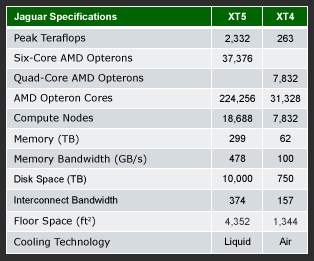
\includegraphics [width=0.55\textwidth, height=0.35\textheight ] {jaguarSpecs09}
  \end{center}
  \caption{Jaguar Machine Specifications \cite{Sciences2010}}
  \label{fig:jaguar}
\end{figure}

While the fastest computer in the world in 2010 may not be the best example of what is standard, machines on which parallel codes can be run are widely available and are becoming faster over time. Access to such machines has changed the landscape of the types of neutron transport problems that can be solved practically. 

Whenever an equation is being mathematically approximated, errors can be introduced that are inherent in the approximation. These errors are present regardless of machine roundoff, phase space discretization, etc. and cannot be changed without changing the approximation. Accepting this mathematical limit as a given, the factor that can be changed to improve calculations is machine architecture. This means that the quality of calculations for a given method is ultimately limited by computers. The research presented here is intended to provide methods that can take full advantage of these new computers, pushing back the frontier of limiting calculations.

%--------------------------------------------------------------------------------
%--------------------------------------------------------------------------------
\section{The Transport Equation}
To understand the methods that were developed for this work and how they will enable the use of leadership-class hardware, the mathematical details of the transport equation must be discussed first. This subsection discusses those details for neutrons in steady-state systems. 

Neutrons can have many different kinds of interactions that influence a system's behavior. These interactions are described by cross sections, which reflect the likelihood of a particular interaction occurring and are given in units of inverse length. Of particular interest is the total cross section, $\Macro$, which includes all possible interactions; the scattering cross section, $\Macro_{s}$, where scattering can change the momentum and kinetic energy of a neutron; and the fission cross section, $\Macro_{f}$.   

Fission is the process through which a nucleus splits into (typically two) smaller atoms. Through this process a relatively large amount of energy is released along with several neutrons. These neutron are available to go on to cause other fissions, creating a chain reaction. The quantity $\nu$ is the average number of neutrons released per fission. Most of the energy released from fission is kinetic, which creates the heat used to make electricity \cite{Lewis1993}.  

If fission is occurring, it is often of interest to know the asymptotic behavior of the system. A reactor is called ``critical'' if the chain reaction is self-sustaining and time-independent. If the system is not in equilibrium then the asymptotic neutron distribution, or the fundamental mode, will grow or decay exponentially over time. A convenient way to capture this behavior is to assume $\nu$ can be adjusted to obtain a time-independent solution by replacing it with $\frac{\nu}{k}$, where $k$ is the parameter expressing the deviation from critical. This substitution changes the transport equation into an eigenvalue problem. A spectrum of eigenvalues can be found, but at long times only the non-negative solution corresponding to the largest real eigenvalue will dominate. The eigenproblem can be written as:
%
\begin{align}
   [\hat{\Omega} \cdot \nabla + \Macro(\vec{r}, E)] \psi(\vec{r}, \hat{\Omega}, E)  &=  \int dE' \int d\hat{\Omega'} \:\Macro_{s}(\vec{r}, E' \to E, \hat{\Omega'} \cdot \hat{\Omega}) \psi(\vec{r}, \hat{\Omega'}, E') \nonumber \\
&+\frac{ \chi(E)}{k} \int dE' \:\nu \Macro_{f}(\vec{r}, E') \int d\hat{\Omega'} \:\psi(\vec{r}, \hat{\Omega'}, E') \:,
\label{eq:neutron transport}
\end{align}

\noindent where the quantities are at location $\vec{r}$, traveling in directions $\hat{\Omega}$, and at energy E and are defined as: \\
\indent $\psi(\vec{r}, \hat{\Omega}, E)$ is the angular neutron flux in neutrons per unit length squared per steradian and expresses where all the neutrons are in phase space, \\
\indent $\chi(E)$ is the fission spectrum and specifies the energy distribution of neutrons born from fission, \\
\indent $k$ is the eigenvalue, which can be thought of as the asymptotic ratio of the number of neutrons in one generation to the number in the next \cite{Lewis1993}.

If fission is not present the transport equation becomes a fixed source rather than eigenvalue problem. The term containing $k$ is replaced by an external source, $q_{ex}(\vec{r}, \hat{\Omega}, E)$, and the equation becomes a standard linear system. 

A brief aside about some properties of the transport equation will aid in understanding the challenge of finding solution techniques that work for all problems of interest. In a void, the transport equation is like a hyperbolic wave equation. For highly-scattering regions where $\Macro_{s}$ is close to $\Macro$, the equation becomes elliptic for the steady-state case. If the scattering is forward-peaked then the equation is parabolic. All of these classes of equations have different solution strategies. The equation is linear, though non-linearities can be introduced if temperature-dependence of cross sections and other similar physics are considered \cite{Adams2002}.  The non-linear considerations are beyond the scope of this work and only the linear case is considered here.

To numerically solve Equation \eqref{eq:neutron transport} it is discretized in space, angle, and energy. This work uses the multigroup approximation, the scattering term is expanded into Legendre polynomials, and discrete ordinates to treat direction of neutron travel. There are many spatial differencing methods available, the discussion of which are beyond the scope of this document as the proposed work is not dependent upon the spatial discretization employed. To ensure the new methods apply to the most general cases it will be assumed that the matrices resulting from discretization are not necessarily symmetric. 

%--------------------------------------------------------------------------------
\subsection{Multigroup Approximation}
The first variable to discretize is energy. In the multigroup approximation, the energy range of interest is broken into $G$ groups. The neutron flux is constant in energy over each group. The groups are ordered such that the highest energy group bound corresponds with $g = 0$, meaning group 1 is defined over $E_{1}$ to $E_{0}$, and the lowest energy bound corresponds with $g = G$. On this grid the group angular flux is defined as: 
%
\begin{equation}
  \psi_{g}(\vec{r},\hat{\Omega}) = \int_{g} dE \:\psi(\vec{r}, \hat{\Omega}, E) = \int_{E_{g}}^{E_{g-1}}dE \:\psi(\vec{r}, \hat{\Omega}, E) \:.
\end{equation}

Justification of this definition comes from assuming the angular flux within each energy group can be approximated by the product of the group flux and a known function: $\psi(\vec{r}, \hat{\Omega}, E) \approx f(E)  \psi_{g}(\vec{r},\hat{\Omega})$ for $E_{g} < E \le E_{g-1}$. The function is normalized for a specific group $g$ such that $\int_{g' = g} dE \:f(E) = 1$ and $\int_{g' \ne g} dE \:f(E) = 0$. The details of $f$ are isotope-dependent and can be garnered from nuclear data. With this notation, group quantities are defined as:

\indent $\Macro_{g}(\vec{r}) = \int_{g} dE \:\Macro(\vec{r}, E) f(E)$, \\
\indent $\nu \Macro_{fg}(\vec{r}) = \int_{g} dE \:\nu \Macro_{f}(\vec{r}, E) f(E)$, \\ 
\indent $\Macro_s^{gg'}(\vec{r}, \hat{\Omega'} \cdot \hat{\Omega}) = \int_{g} dE \:\int_{g'} dE' \:\Macro_{s}(\vec{r}, E' \to E, \hat{\Omega'} \cdot \hat{\Omega})  f(E')$ is the scattering from $g'$ into $g$, \\
\indent $\chi_{g} = \int_{g} dE \:\chi(E)$, and \\
\indent $q^{e}_{g}(\vec{r}, \vOmega) = \int_{g} dE \:q_{ex}(\vec{r}, \hat{\Omega}, E)$.

\noindent Using these terms, the eigenvalue form of Equation \eqref{eq:neutron transport} can be rewritten for each group $g$ as seen in \eqref{eq:group-transport} \cite{Lewis1993}. Using more energy groups represents the physics in the cross sections more accurately, but also increases the cost of a calculation in terms of both operations and storage. 
% 
\begin{align}
   [\hat{\Omega} \cdot \nabla + \Macro_{g}(\vec{r})] \psi_{g}(\vec{r}, \hat{\Omega})  &=  \sum_{g'=1}^{G} \int d\hat{\Omega'} \:\Macro_s^{gg'}(\vec{r}, \hat{\Omega'} \cdot \hat{\Omega}) \psi_{g'}(\vec{r}, \hat{\Omega'})  \nonumber \\
&+ \frac{\chi_{g}}{k}   \sum_{g'=1}^{G} \nu \Macro_{fg'}(\vec{r}) \int d\hat{\Omega'} \:\psi_{g'}(\vec{r}, \hat{\Omega'}) 
\label{eq:group-transport}
\end{align}

%--------------------------------------------------------------------------------
\subsection{Scattering Discretization}
In Equation \eqref{eq:group-transport} the scattering cross section is a complicated function of angle. Simplifying this term will make the system easier to solve. Because of rotational symmetry of nuclear collisions, $\Macro_{s}$ is only a function of the cosine between the incoming and outgoing angles. This allows the scattering cross section to be written as a series expansion of Legendre polynomials as follows, where the the spatial variable has been supressed:
%
\begin{equation}
  \sigg{}(\vOmega' \cdot \vOmega) = \sum_{l=0}^{N} \frac{2l+1}{4\pi} P_{l}(\vOmega' \cdot \vOmega)\sigg{l} \:.
\end{equation}

The addition theorem of spherical harmonics can be used to evaluate the Legendre function, $P_{l}(\vOmega' \cdot \vOmega)$ with spherical harmonic terms, $Y_{lm}$. These can then be expanded into real and imaginary components. The imaginary components must be zero since scattering must be real. All of this gives:
%
\begin{equation}
  P_l(\vOmega' \cdot \vOmega) = \frac{4\pi}{2l+1} \Bigl[ Y^e_{l0}(\vOmega) Y^e_{l0}(\vOmega') + \sum_{m=1}^l \bigl( Y^e_{lm}(\vOmega) Y^e_{lm}(\vOmega') + Y^o_{lm}(\vOmega) Y^o_{lm}(\vOmega') \bigr) \Bigr]\:.
\end{equation}
%
The $Y^e$ and $Y^o$ terms obey the following orthogonality relationships: $\int d\vOmega \:Y^{e}_{lm}(\vOmega)Y^{e}_{l'm'}(\vOmega) = \frac{1}{2}(1 + \delta_{m0})\delta_{ll'}\delta_{mm'}$ and $\int d\vOmega \:Y^{o}_{lm}(\vOmega)Y^{o}_{l'm'}(\vOmega) = \frac{1}{2}(1 - \delta_{m0})\delta_{ll'}\delta_{mm'}$. The spherical harmonics therefore form an orthonormal basis in which the Legendre polynomials are expressed \cite{Evans2009}, \cite{Lewis1993}. 

By putting all of this information together, the scattering source can be expressed as: 
%
\begin{equation}
  q^g_{s} (\vec{r}, \vOmega) = \sum_{g'=1}^G \sum_{l=0}^N \sigg{l}(\vec{r}) \Bigl[ Y^e_{l0}(\vOmega) \evenp_{l0}(\vec{r}) + \sum_{m=1}^l \bigl( Y^e_{lm}(\vOmega) \evenp_{lm}(\vec{r}) + Y^o_{lm}(\vOmega) \oddp_{lm}(\vec{r}) \bigr) \Bigr]\:.
   \label{eq:mg-scattering-source}
\end{equation}
%
In Equation \eqref{eq:mg-scattering-source} two terms, called the even and odd flux moments, have been used:
%
\begin{alignat}{3}
  \even_{lm} &= \int_{4\pi} d\vOmega' \:Y^e_{lm}(\vOmega') \psi^g(\vOmega') \:, \quad& m\ge 0\:,\qquad \text{even} \:, \label{eq:even-flux}\\
  %
  \odd_{lm} &= \int_{4\pi} d\vOmega' \:Y^o_{lm}(\vOmega')\psi^g(\vOmega') \:, \quad& m>0 \:,  \qquad \text{odd} \label{eq:odd-flux} \:.
\end{alignat}
%
The external source can be similarly discretized if desired, making the two sources consistent with one another. The full details of these expansions and bases can be found in \cite{Evans2009}. 

The multigroup, anisotropic scattering source found in Equation \eqref{eq:mg-scattering-source} is characterized by the order of Legendre scattering, $P_{N}$. For a given Legendre expansion there are $(N + 1)^{2}$ flux moments. Using more moments represents scattering more accurately, but increases the cost of a calculation \cite{Evans2009}.  

%--------------------------------------------------------------------------------
\subsection{Discrete Ordinates Approximation}
The next area of phase space to discretize is direction. The discrete ordinates or \Sn approximation is a collocation method that is used to express the transport equation on a discrete set of $n$ ordinates, where the ordinates are described by angles and represent direction of neutron travel. A collocation method represents a continuous function on a finite set of collocation points using a linear combination of basis functions. The approximate solution must satisfy the differential equation at those collocation points \cite{Heath2002}. 

For the transport equation, the basis functions are the angular fluxes along specific directions and the collocation points are the angle sets. The linear combination is done by weighting the basis functions using a quadrature set. 

To implement this, the transport equation is written for neutrons traveling in $d\vOmega$ about direction $\vOmega_{a}$. Now $\psi^{g}_{a}$ can be defined as $\psi^{g}(\vOmega_{a})$, and the angular flux can be related to the flux moments as $\phi^{g} = \sum_{a=1}^{n}\psi^{g}_{a}w_{a}$. Using these terms, including the discretized scattering source, and suppressing spatial dependence, Equation \eqref{eq:group-transport} becomes:
%
\begin{align}
 \bigl( \vOmega_{a} \cdot \nabla + \Macro_{g} \bigr) \psig_{a} = \sum_{g' = 1}^{G} \sum_{l=0}^{N} \sigg{l} \bigl[ Y^{e}_{l0}(\vOmega_{a}) \evenp_{l0} &+ \sum_{m=1}^{l} \bigl( Y^{e}_{lm}(\vOmega_{a}) \evenp_{lm} + Y^{o}_{lm}(\vOmega_{a}) \oddp_{lm} \bigr) \bigr] \nonumber \\
 &+ \frac{\chi^{g}}{k} \sum_{g'=1}^{G} \nu \Macro_{f}^{g'}\phi^{g'} \:,
  \label{eq:mg-sn-transport}
\end{align}

The quadrature weights, $w_{a}$, are defined such that $\int_{4 \pi} d\vOmega =  \sum_{a=1}^{n}w_{a} = 4 \pi$. One of the choices in the \Sn approximation is what quadrature set to use and the number of unknowns contributed by discretization of direction is determined by the quadrature set. For example, level-symmetric quadrature gives $n = N(N+2)$ unknowns for an \Sn approximation. The flux moments are also collocated on the ordinates using the desired quadrature set to linearly combine the angular flux basis functions \cite{Evans2009}:
%
\begin{align}
  \even_{lm} &= \sum_{a=1}^{n}Y^e_{lm}(\vOmega'_a)\psi^g_a w_a\:,
  \label{eq:even-flux-quad-int}\\
  \odd_{lm} &= \sum_{a=1}^{n}Y^o_{lm}(\vOmega'_a)\psi^g_a w_a\:.
  \label{eq:odd-flux-quad-int}
\end{align}

%--------------------------------------------------------------------------------
\subsection{Operator Form}
Now that the transport equation has been discretized, it can be expressed in operator notation. Using the operator form of the transport equation will facilitate the presentation of the solution techniques discussed in the remainder of this document. In general, uppercase bolded letters will indicate matrices and lowercase italicized letters will indicate vectors and scalars. The following operators are used to express the transport equation:\\
%
\indent $\mathbf{L} = \vOmega \cdot \nabla + \Macro$ is the transport operator, \\
\indent $\mathbf{M}$ is the operator that converts harmonic moments into discrete angles, \\
\indent $\mathbf{S}$ is the scattering matrix, \\
\indent $f$ contains the fission source, $\nu \Macro_{f}$; $\mathbf{F} =\mathbf{\chi} f^{T}$, \\ 
\indent $\mathbf{D} = \ve{M^{T}}\ve{W} = \sum_{a=1}^{n}Y^{e/o}_{lm}w_{a}$ is the discrete-to-moment operator. 

With this notation Equation \eqref{eq:mg-sn-transport} can be written as \eqref{eq:operator-form}; it can be formulated as a fixed source problem by replacing the fission term with $\ve{M}q_{e}$. This has two unknowns, the angular flux and the moments, which are related by the discrete-to-moment operator as seen in Equation \eqref{eq:moments}.
%
\begin{align}
  \mathbf{L} \psi &= \mathbf{MS}\phi + \frac{1}{k}\mathbf{MF}\phi \label{eq:operator-form}\\
  \phi &= \mathbf{D}\psi 
  \label{eq:moments}
\end{align}
The typical strategy for solving Equation \eqref{eq:operator-form} is to combine it with \eqref{eq:moments} and form one equation involving only the moments, where $Q$ is comprised of the fixed or fission source: 
\begin{equation}
   (\ve{I} - \ve{DL}^{-1}\ve{MS})\phi = Q \:.
\end{equation}  
This is solved for $\phi$ from which $\psi$ can be determined at the end of the calculation.

The size of the operators can be defined in terms of the granularity of discretization: \\
%
\indent $G$ = number of energy groups, \\
\indent $t$ = number of moments, \\
\indent $n$ = number of angular unknowns, \\
\indent $c$ = number of cells, \\
\indent $u$ = number of unknowns per cell, which is determined by spatial discretization. \\
%
These can be combined to define $a = G \times n \times c \times u$ and $f = G \times t \times c \times u$. Using $a$ and $f$, Equation \eqref{eq:operator-form} can be presented in terms of operator size: $(a \times a)(a \times 1) = (a \times f) (f \times f) (f \times 1) + (a \times f) (f \times f) (f \times 1)$. The index variables, their meaning, and their ranges are shown in Table \ref{table:index}. 
%
\begin{table}[!h]
\caption{Meaning and Range of Indices Used in Transport Discretization}
\begin{center}
\begin{tabular}{l c c c c}
\hline
Variable & Symbol & First & Last \\[0.5ex]
\hline
Energy & g & 1 & G \\
Solid Angle & a & 1 & n \\
Space & suppressed & n/a & n/a \\
Legendre moment ($P_{N}$) & $l$ & 0 & N \\
Spherical harmonic moment ($Y$) & m & 0 & $l$ \\
\hline
\end{tabular}
\end{center}
\label{table:index}
\end{table}
%

The structures of the vectors and matrices are shown in the next few equations as this will make some of the proposed methods easier to understand and visualize \cite{Evans2009}. The angular flux vector is explicitly written first, where for each discrete angle, $a$, and energy group, $g$, the set of angular fluxes, $ \psi^g_a$, includes all spatial unknowns.
%
 \begin{align}
    \psi &=     \begin{pmatrix}
    [\psi]_{1} & [\psi]_2 & \cdots & [\psi]_g & \cdots [\psi]_{G} 
  \end{pmatrix}^T  \:, \qquad \text{and} \nonumber \\
  %
    [\psi]_g &= \begin{pmatrix}
    \psi^g_1 & \psi^g_2& \cdots & \psi^g_a & \cdots \psi^g_n 
  \end{pmatrix}^T \:.  \nonumber 
\end{align}
%
\begin{alignat}{2}
  \mathbf{M} &=    \begin{pmatrix}
      [\ve{M}]_{11} & 0 & 0 & \cdots & 0 \\
      0 & [\ve{M}]_{22} & 0 & \cdots & 0 \\
      0 & 0 & [\ve{M}]_{33} & \cdots & 0 \\
      \vdots & \vdots & \vdots & \ddots   & \vdots \\
      0 & 0 & 0 & \cdots & [\ve{M}]_{GG} \\
    \end{pmatrix} \nonumber  \:,& \qquad
    %
  \mathbf{S}  =     \begin{pmatrix}
      [\ve{S}]_{11} & [\ve{S}]_{12} & [\ve{S}]_{13} & \cdots &
      [\ve{S}]_{1G} \\
      [\ve{S}]_{21} & [\ve{S}]_{22} & [\ve{S}]_{23} & \cdots &
      [\ve{S}]_{2G} \\
      [\ve{S}]_{31} & [\ve{S}]_{32} & [\ve{S}]_{33} & \cdots &
      [\ve{S}]_{3G} \\
      \vdots & \vdots & \vdots & \ddots & \vdots \\
      [\ve{S}]_{G1} & [\ve{S}]_{G2} & [\ve{S}]_{G3} & \cdots &
      [\ve{S}]_{GG}
    \end{pmatrix} \nonumber  \:,
 \end{alignat}
 %
 \begin{alignat}{2}
      \mathbf{F}  &=     \begin{pmatrix}
     \chi^{1}[\nu\Macro_{f}]^{1} &\chi^{1}[\nu\Macro_{f}]^{2} & \cdots &
      \chi^{1}[\nu\Macro_{f}]^{G} \\
      \chi^{2}[\nu\Macro_{f}]^{1} &\chi^{2}[\nu\Macro_{f}]^{2} & \cdots &
      \chi^{2}[\nu\Macro_{f}]^{G}\\
      \vdots & \vdots & \ddots & \vdots \\
      \chi^{G}[\nu\Macro_{f}]^{1} &\chi^{G}[\nu\Macro_{f}]^{2} & \cdots &
      \chi^{G}[\nu\Macro_{f}]^{G}\\
    \end{pmatrix} \:, \nonumber & \qquad
    %
  [\ve{S}]_{gg'} = \begin{pmatrix}
    \sigg{0} & 0 & \cdots & 0  \\
    0 & \sigg{1} & \cdots & 0 \\
    \vdots & 0 & \ddots  & \vdots \\
     0 & 0 & \cdots & \sigg{N}
  \end{pmatrix}\:, \nonumber
 \end{alignat}
    %
\begin{equation}    
   [\ve{M}]_{gg} = \begin{pmatrix}
    \Ye{00}{1} & \Ye{10}{1} & \Yo{11}{1} & \Ye{11}{1} & 
    \Ye{20}{1} & \cdots & \Yo{NN}{1} & \Ye{NN}{1} \\
    \Ye{00}{2} & \Ye{10}{2} & \Yo{11}{2} & \Ye{11}{2} & 
    \Ye{20}{2} & \cdots & \Yo{NN}{2} & \Ye{NN}{2} \\
    \Ye{00}{3} & \Ye{10}{3} & \Yo{11}{3} & \Ye{11}{3} & 
    \Ye{20}{3} & \cdots & \Yo{NN}{3} & \Ye{NN}{3} \\
    \vdots     & \vdots     & \vdots     & \vdots     & 
    \vdots     &  \ddots    & \vdots     & \vdots     \\
    \Ye{00}{n} & \Ye{10}{n} & \Yo{11}{n} & \Ye{11}{n} & 
    \Ye{20}{n} & \cdots & \Yo{NN}{n} & \Ye{NN}{n}
  \end{pmatrix}\:. \nonumber \\
\end{equation}

\noindent Note that $[\ve{M}]_{11} = [\ve{M}]_{22} =  \hdots = [\ve{M}]_{GG} = [\ve{M}]$. These are written with subscripts to simplify the visualization of which blocks correspond to which equations and multiply which other blocks. 

%--------------------------------------------------------------------------------
\subsection{Solution Procedure}
Once the matrices are multiplied together, a series of single-group equations that are each only a function of space and angle result:
%
\begin{equation}
  \begin{aligned}
    \ve{L}[\psi]_1 &= [\ve{M}]\bigl([\ve{S}]_{11}[\phi]_1 + 
    [\ve{S}]_{12}[\phi]_2 + \ldots + [\ve{S}]_{1G}[\phi]_G\bigr) + 
    \frac{1}{k}[\ve{M}]\sum_{i=1}^{G}[\ve{F}]_{1i}[\phi]_{i} \:, \\
    %%
    \ve{L}[\psi]_2 &= [\ve{M}]\bigl([\ve{S}]_{21}[\phi]_1 + 
    [\ve{S}]_{22}[\phi]_2 + \ldots + [\ve{S}]_{2G}[\phi]_G\bigr) + 
     \frac{1}{k}[\ve{M}]\sum_{i=1}^{G}[\ve{F}]_{2i}[\phi]_{i} \:, \\
    %%
    &\vdots\\
    %%
    \ve{L}[\psi]_G &= [\ve{M}]\bigl([\ve{S}]_{G1}[\phi]_1 + 
    [\ve{S}]_{G2}[\phi]_2 + \ldots + [\ve{S}]_{GG}[\phi]_G\bigr) + 
     \frac{1}{k}[\ve{M}]\sum_{i=1}^{G}[\ve{F}]_{Gi}[\phi]_{i} \:.
  \end{aligned}
  \label{eq:group-equations}
\end{equation}
%
Each ``within-group'' equation is solved for that group's flux. If the groups are coupled together, as they often are, then multiple ``multigroup'' solves over the coupled portion of the energy range may be required. If the eigenvalue is desired an additional ``eigenvalue'' solve is needed as well \cite{Evans2009}. The details of these steps will be discussed later as they relate to the new methods.  


%--------------------------------------------------------------------------------
%--------------------------------------------------------------------------------
\section{Meeting the Goal}
The fully discretized steady-state transport equation can become very large when trying to solve ``grand challenge'' types of problems. The continued improvement of computational resources has enabled the invention of massively parallel codes designed to work on leadership-class computers. The goal of this work is to develop and implement new methods that will accelerate transport calculations by efficiently taking advantage of cutting-edge computer architectures. 

The code being used in this work is Denovo \cite{Evans2009}, a massively parallel discrete ordinates code being developed at Oak Ridge National Laboratory. The code allows multiple combinations of spatial discretizations, quadrature sets, and solution methodologies. Denovo is three-dimensional, uses a non-uniform, structured, Cartesian grid, has a flexible front end, and is capable of writing and reading input parameters rapidly for high performance computing. 

At the outset of this work, Denovo could be decomposed for parallel computation in five of the six dimensions of phase space over which the steady-state transport equation is solved. The nature of the decomposition dictated how many cores Denovo could use efficiently. Studies to be discussed in Chapter \ref{sec:Chp2} illustrate that the number of cores was not sufficient to solve the real problems of interest. 

The original suite of solvers in Denovo included Source Iteration (SI) and Krylov as within group solvers, Gauss-Seidel (GS) as a multigroup solver, and power iteration (PI) as an eigenvalue solver. These solvers have some significant limitations in many cases of interest. Each method and its associated challenges will be described in detail in following chapters. 

Significant acceleration of Denovo has been accomplished by implementing three complimentary solution strategies. The first is a multigroup solution option that allows the energy groups to be decomposed for fixed source problems. The solver allows Denovo to be decomposed in energy such that multigroup solves can be parallelized in the energy dimension. This addition lets Denovo to take advantage of many more cores without significantly degrading the scaling. The \emph{multigroup Krylov solver} also converges more quickly than Gauss Seidel. This work is discussed in Chapter~\ref{sec:Chp2}.

The second strategy was to add an eigenvalue method with convergence properties that can be superior to power iteration, particularly for loosely coupled problems. \emph{Rayleigh Quotient Iteration} (RQI) applies a shift to the equations that improves the eigenvalue convergence properties. The shift also increases the degree of group-to-group coupling. The multigroup Krylov solver enables RQI because it solves coupled groups efficiently and decomposes coupled groups for energy parallelization. The details of this work are discussed in Chapter~\ref{sec:Chp3}.

The third step was to add a new physics-based preconditioner that is a multigrid method in energy. This capitalizes on the energy decomposition added by the first method. Since energy groups can be treated independently, they can be combined and re-separated in a multi-grid like fashion very easily. The preconditioner is applicable to both fixed source problems and eigenvalue calculations, and it reduces the number of iterations required for convergence in all cases. The \emph{multigrid in energy preconditioner} is discussed in Chapter~\ref{sec:Chp4}.

Fast and scalable codes are necessary for solving truly large and challenging neutron transport problems. This work developed methods that accelerated an existing transport code by allowing it to scale to hundreds of thousands of cores and converge more quickly than the previous methods, thus enabling the development of new and useful nuclear energy systems. These methods may also be beneficial for the larger computational community.

\separatorpage{}  
                 % Chapter 1. ``Introduction and Motivation''
 % Prelim, Chapter 2
% by Rachel Slaybaugh

\chapter{Upscattering and Energy Decomposition}
\label{sec:Chp2}
The first piece that was added to Denovo to accelerate the code was the multigroup Krylov solver. The second two methods rely on the energy decomposition and improved convergence added by this solver, so its functionality is essential to all subsequent work. The multigroup Krylov solver works very well and is a key element in accomplishing the goals of this work. 

First, the limitations of the existing parallel decomposition in Denovo for solving challenging problems are explained. Next, the background section discusses scattering and some solver basics, including an overview of Krylov subspace methods and why they are of interest for solving the transport equation. The next section focuses on existing methods used to solve the fixed source transport equation and relevant past work. Finally, a description of the new method and associated results are presented.

\section{Denovo and Parallelism}
\label{sec:DenAndPar}
To be able to solve the very large problems of interest on machines the size of Jaguar, codes that have good scaling properties are required. Recall that Denovo is parallelized in space and angle. This is done with the Koch-Baker-Alcouffe (KBA)~\cite{Baker1998} parallel sweep algorithm on a Cartesian grid. The KBA algorithm governs Denovo's parallel behavior, including how many cores it can efficiently use. To see why parallelization in energy is needed, the KBA algorithm is explained and some illustrative Denovo calculations are presented.

Angular parallelization is done by algorithmically ``stacking'' the calculation directions (ordinates) into a ``pipe'' and following more than one at a time. The transport sweeps begin with the first direction in the first quadrant and spatially move through the geometry along that ordinate in a hyper-plane fashion. Denovo uses a pipelining approach in direction such that the next angle set in an octant is started as soon as the current sweep reaches the opposite end of the geometry. The quadrants are ordered such that the next quadrant begins at the earliest possible time \cite{Evans2009d}. 

The spatial decomposition is done by assigning groups of spatial cells to different cores. A given problem will contain $(I, J, K)$ total global \emph{cells}. These are decomposed in $x$ and $y$ across $P_{I}$ cores in the $x$-direction and $P_{J}$ cores in the $y$-direction for a total of $P_{I} \times P_{J}$ cores. Each core gets a \emph{domain} that is made up of $(I_{b}, J_{b}, K)$ cells. Here $I_{b} = I/P_{I}$ and $J_{b} = J/P_{J}$. Each domain is algorithmically split into $B_{K}$ computational blocks in the $z$-direction (but not split in memory, all $K$ cells in the $z$-direction are on all cores). This creates \emph{computational blocks} of size $(I_{b}, J_{b}, K_{b})$, where $K_{b} = K/B_{K}$. The computational blocks are used in the angular pipelining process. Specifying the number of cores dictates $P_{I}$ and $P_{J}$, while the user is free to select $B_{K}$. See Figure \ref{fig:BlockDecomp} for an example of a decomposition.

\begin{figure}[!ht]	
  \begin{center}
    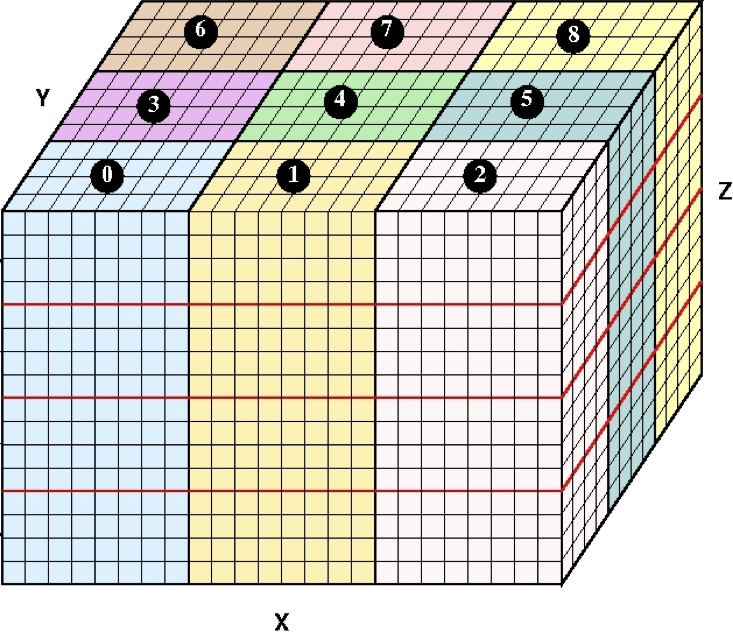
\includegraphics [width=0.6\textwidth, height=0.4\textheight ] {BlockDecompCropped}
  \end{center}
  \caption{Decomposition of 3-D mesh for KBA. In this example, the grid is decomposed on nine processors. The red lines indicated computational blocks in the $z$-direction. Each processor has $I_{b} \times J_{b} \times K$ cells, and each computational block has size $I_{b} \times J_{b} \times K_{b}$.}
  \label{fig:BlockDecomp}
\end{figure}

The decomposition parameters can be used to express the theoretical efficiency of the algorithm, which is the ratio of useful computations to total computations \cite{Evans2009d}, \cite{Baker1998}:
%
\begin{equation}
  \epsilon_{max} = \frac{2MB_{K}}{2MB_{K} + P_{I} + P_{J} - 2} \:, 
  \label{eq:efficiency}
\end{equation}
%
where $M$ is the number of directions in an octant. Note that for a set $M$, $P_{I}$, and $P_{J}$, the theoretical efficiency will be much higher when there is a larger $B_{K}$, meaning more computational blocks. Having more computational blocks creates blocks that are smaller, so work can be passed to subsequent blocks more rapidly and thus more work should be able to be done at once. The effect of $B_{K}$ on theoretical performance can be seen in the strong scaling study shown below. See \cite{Baker1998} for more details about the KBA algorithm.

The quality of parallelization can be measured in several ways. Strong scaling measures how the time to solution varies with the number of cores for a fixed problem size. Weak scaling measures how the time to solution varies with the addition of more cores when the problem size per core is fixed \cite{Bush2010}. Another factor is the total number of cores that can be used efficiently. 

A weak scaling study was performed by Evans et.\ al.\ on the Jaguar machine using a full-facility pressurized water reactor model, called the PWR900. The base-case time was generated using 4,096 cores with 103,716,288 unknowns, or $\sim$25,300 unknowns/core. When 40,000 cores and 1,046,879,390 unknowns ($\sim$26,200 unknowns/core or about a 3\% increase in problem size/core) were used, there was a 43\% increase in time to solution. The time increase for perfect weak scaling would have been about 3\%. The significant increase in time can be attributed to load-balancing latencies associated with KBA \cite{Evans2009d}. Adding parallelization over energy might improve the weak scaling properties of Denovo by making up for some of the latencies that come from KBA.

A strong scaling study was done as a part of this work that used the Jaguar machine to investigate the effect of $B_{K}$ on efficiency. A variant of the Kobayashi benchmark problem 1 \cite{Kobayashi2000}, which can be seen in Figure~\ref{fig:Kob1}, was used where the total cross sections were changed as indicated in Table~\ref{tab:Kob1xsecs}. The scattering cross sections were simply set to 0.5 $\times \Macro$ in both the original and modified case. The calculation was done with $S_{16}$, $P_{0}$, step characteristic spatial differencing, and a 0.25 cm spatial resolution, giving a 400 $\times$ 400 $\times$ 400 mesh. The number of cores was varied between 12 and 3,600. 

\begin{figure}[!ht]	
  \begin{center}
    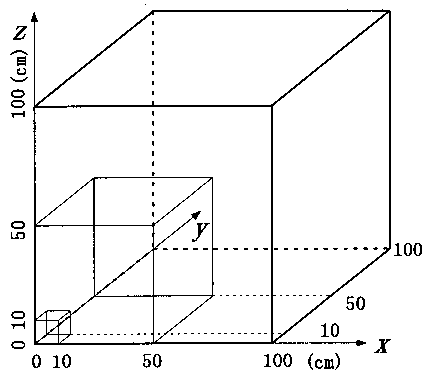
\includegraphics [width=0.4\textwidth, height=0.3\textheight ] {Kobayashi1} \\
    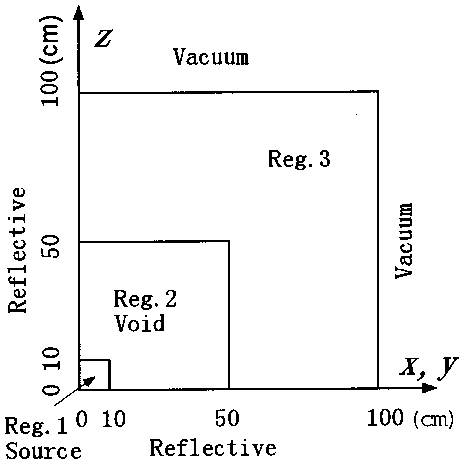
\includegraphics [width=0.4\textwidth, height=0.3\textheight ] {Kobayashi1Front}
  \end{center}
  \caption{Kobayashi Benchmark Problem 1, Two Views}
  \label{fig:Kob1}
\end{figure}

\begin{table}[h]
  \caption{Kobayashi Benchmark Problem 1, Cross Sections and Sources}
  \centering
  \begin{tabular}{|c|c|c|c|}
    \hline
    Region & S & Original $\Macro$ & Modified $\Macro$ \\
    (\#) & ($n$ cm$^{-3}$s$^{-1}$) & (cm$^{-1}$) & (cm$^{-1}$) \\
    \hline
    1 & 1 & 0.1 & 1 \\
    2 & 0 & 10$^{-4}$ & 10$^{-3}$ \\
    3 & 0 & 0.1 & 1 \\
    \hline
  \end{tabular}
  \label{tab:Kob1xsecs}
\end{table}

One set of calculations was done using $B_{K}$ = 40, or relatively many blocks, and one set using $B_{K}$ = 5, or relatively few blocks. Recall from Equation \eqref{eq:efficiency} that more computational blocks should give higher efficiency. The theoretical and actual results are plotted in Figure~\ref{fig:JagBlockStudy} as computational efficiency as a function of the number of cores used. The actual efficiency is $\frac{N_{ref}t_{ref}}{Nt}$. Here $N_{ref}$ and $t_{ref}$ are the reference number of cores and solve time, respectively, and $N$ and $t$ are for the calculation in question.  The theoretical efficiency was calculated using Equation \eqref{eq:efficiency}.

\begin{figure}[!h]
  \begin{center}
    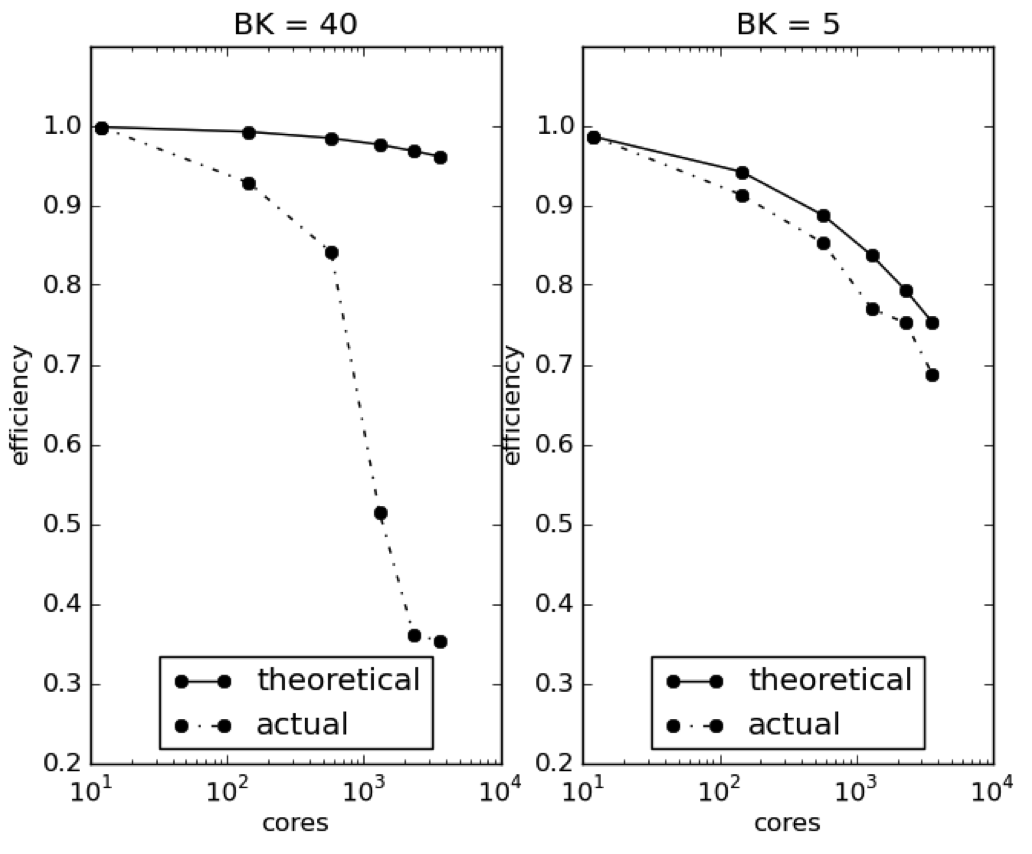
\includegraphics [width=.85\textwidth, height=0.5\textheight ] {JagBlockStudy}
  \end{center}
  \caption{Modified Kobayashi Benchmark Problem 1, Efficiency as a Function of Number of Cores}
  \label{fig:JagBlockStudy}
\end{figure}

A few important conclusions can be drawn from the curves in Figure~\ref{fig:JagBlockStudy}. One is that the increase in simultaneous work that should come from using smaller computational blocks is overwhelmed by communication latency in practice. When $B_{K}$ = 40 the theoretical efficiency remains high as the number of cores increases, but the measured efficiency becomes quite low: for 3,600 cores $\epsilon_{max}$ = 0.96 and $\epsilon$ = 0.35. It is expected that more blocks would be better, but when the number of cells/block becomes too small the cores spend more time waiting to pass data than doing useful work. 

Another relevant finding is that the theoretical and actual efficiencies match when there is a minimum block size. When larger computational spaces are used (smaller $B_{K}$) communication does not become a dominant factor. This restricts the extent of spatial decomposition by limiting the number of blocks used for a given spatial mesh. For a 500M cell problem, the limitation is 15,000 - 20,000 cores. 

Once a problem is spatially decomposed beyond the minimum block size limit, communication latency begins to dominate solution time and using more cores will be of little benefit. This is caused by the KBA algorithm. In order to take advantage of more cores for a given problem size, another area of phase space must be parallelized: energy, the remaining unparallelized dimension. 

It is worth noting that the phrase ``for a given problem size'' is important when stating that a problem cannot efficiently use more cores by being further decomposed in space alone. If a system is meshed more and more finely, then more cores can be used. For problems of interest today, however, using meshes large enough to use the full Jaguar machine efficiently necessitates meshing beyond discretizations of physical interest in nuclear engineering. 

One last point is that the current decomposition only allows for refining a problem in space and angle to increase parallelization and keep the wall time low as problems get larger. More finely resolving energy, which is desired for many of today's calculations, only makes the problem more expensive. No matter what mesh is used, KBA will never be able to use of more cores to get better energy resolution.

%--------------------------------------------------------------------------------
%--------------------------------------------------------------------------------
\section{Background}
To understand the new method and why it enhances Denovo's performance, this section contains an explanation of scattering, an overview of relevant basic solvers, and information about how scattering is treated in the transport equation. The remainder of this chapter will primarily focus on the solution of $\ve{A}x = b$, where $\ve{A}$ is $n \times n$  and the exact form of $\ve{A}$ and $b$ will be specified in subsequent sections.

%--------------------------------------------------------------------------------
\subsection{Scattering}
One of the important contributions of this work is the implementation of a new mathematical approach for upscattering in transport calculations. When neutrons scatter, several outcomes with regard to energy are possible. One outcome is that neutrons can stay within their energy group, called within-group scattering, and is described by the $[\ve{S}]_{gg}$ portion of the scattering matrix. Neutrons can also move into a lower energy group, or downscatter, given by $[\ve{S}]_{gg'}$ where $g > g'$. In some cases neutrons can gain energy and upscatter, described by $[\ve{S}]_{gg'}$ where $g < g'$. 

Material cross sections can be highly energy dependent and therefore high-resolution data in certain energy ranges may be needed to accurately capture the physics of the system. Upscattering is often important in problems where detailed information about low-energy, or thermal, neutrons is needed. In light-water reactors, thermal neutrons cause the bulk of the fission so these are systems that often need cross sections with upscattering terms.  

As mentioned in Chapter \ref{sec:Chp1}, the transport problem is broken into outer iterations and inner iterations. The inner iterations correspond to the within-group equations. Each inner iteration converges the flux for just one group by solving a fixed source problem for that group. The fixed source contains the appropriate combination of inscattering from other groups, an external source, and a source from fission.  The outer iterations are over the entire set of energy groups: all of Equations \eqref{eq:group-equations}. If a problem does not have upscattering, the equations can be quickly solved using one outer iteration. 

%--------------------------------------------------------------------------------
\subsection{Solver Basics}
There are two categories of methods for solving $\ve{A}x = b$, direct and iterative. Direct methods solve the problem by inverting $\ve{A}$ and setting $x = \ve{A}^{-1}b$. If $\ve{A}$ is invertible this can be done explicitly. $\ve{A}$ is often not invertible, so most direct methods are based on factoring the coefficient matrix $\ve{A}$ into matrices that are easy to invert. The problem is then solved in pieces where each factored matrix is inverted to get the final solution. An example where this is done is LU factorization. These methods are often robust and require a predictable amount of time and storage resources. However, direct methods scale poorly with problem size, becoming increasingly expensive as problems grow large \cite{Benzi2002}.

Iterative methods compute a sequence of increasingly accurate approximations to the solution. They generally require less storage and take fewer operations than direct methods, though they may not be as reliable. Iterative methods are highly advantageous for large problems because direct methods become intractable for systems of the size of those of interest here. For this reason the nuclear energy industry tends to use iterative methods for transport calculations \cite{Birkhoff1984}, \cite{Benzi2002}. 

Within the category of iterative methods, two further subdivisions can be made that will be useful in this work. Some methods only place data from previous iterations on the right hand side of the equation. The order in which those equations are solved is then irrelevant because only the previous iterate is needed. The other class of methods place data from both the previous and current iteration on the right hand side. These methods are fundamentally sequential and must be solved in order. These two categories will be referred to as order independent and order dependent, respectively. 

\subsubsection{Richardson Iteration}
The simplest iteration scheme used by the nuclear community is source iteration (SI), also known as Richardson iteration. SI is applied to the within-group space-angle iterations. Some other method is needed to conduct outer iterations over energy. Richardson iteration can be thought of as a two-part process for the neutron transport equation, where $\bar{Q}$ includes all sources and $k$ is the inner iteration index:
%
\begin{align}
  \ve{L}[\psi]_g^{k+1} &= \ve{MS} [\phi]_g^k + [\bar{Q}]_{g} \:,   \label{eq:SIpsi} \\
  [\phi]_g^{k+1} &= \ve{D}[\psi]_g^{k+1} \:.
  \label{eq:SIphi}
\end{align}
%
The spectral radius determines the speed of convergence and is $c = \Macro_s / \Macro$. For problems dominated by scattering, SI will converge very slowly \cite{Evans2009d}. While this is the simplest iterative method used, there are other more sophisticated methods available. 

\subsubsection{Jacobi}
The Jacobi method is known as the method of simultaneous displacements \cite{LeVeque2007}. This could be applied as the outer iteration method over energy and can be written as follows where $j$ is the outer iteration index:
%
\begin{equation}
  \ve{L} [\psi]_{g}^{j+1} = [\ve{M}] [\ve{S}]_{gg}[\phi]_{g}^{j} +   [\ve{M}]\bigl(\sum_{g'=1}^{g-1} [\ve{S}]_{gg'}[\phi]_{g'}^{j} + \sum_{g'=g+1}^{G} [\ve{S}]_{gg'}[\phi]_{g'}^{j} + [q_{e}]_{g} \bigr) \label{eq:Jacobi} \:. 
\end{equation}
%
The Jacobi method is order independent since all terms on the right are at the old iteration level. Jacobi is unconditionally stable and linearly convergent, but may converge very slowly. The convergence of Jacobi is governed by its spectral radius \cite{LeVeque2007}. 

\subsubsection{Gauss Seidel}
Gauss Seidel (GS) is known as the method of successive displacements \cite{LeVeque2007}. It is commonly used as the outer iteration method over energy and can be written as follows:
%
\begin{equation}
  \ve{L} [\psi]_{g}^{j+1} = [\ve{M}] [\ve{S}]_{gg}[\phi]_{g}^{j+1} +   [\ve{M}]\bigl(\sum_{g'=1}^{g-1} [\ve{S}]_{gg'}[\phi]_{g'}^{j+1} + \sum_{g'=g+1}^{G} [\ve{S}]_{gg'}[\phi]_{g'}^{j} + [q_{e}]_{g} \bigr) \label{eq:GaussSeidel} \:. 
\end{equation}
%
The GS method is order dependent, containing terms on the right hand side at both the new and old iterates. Once the space-angle iterations for each upscattering group are completed for one outer iteration, the right hand side is recalculated and the within-group calculations are repeated. This goes on until the entire system converges \cite{Evans2009d}. 

Gauss Seidel is also unconditionally stable and linearly convergent, but may converge very slowly. The convergence of GS is also governed by its spectral radius, $\rho$, though it converges twice as fast as the Jacobi method \cite{LeVeque2007}. 

The spectral radius of Gauss Seidel has been found for various materials by solving the eigenvalue problem $(\ve{T} - \ve{S}_{D})^{-1}\ve{S}_{U} \xi = \rho \xi$, where $\ve{T}$ is the matrix of total cross sections, $\ve{S}_{U}$ is the upper triangular portion of $\ve{S}$, $\ve{S}_{D}$ contains the diagonal and lower triangular portion, and $\xi$ is the eigenvector. This eigenvalue problem comes from Fourier analysis. The spectral radii for some materials of practical interest determined using cross sections with 41 thermal upscattering groups are: graphite = 0.9984, heavy water = 0.9998, and iron = 0.6120 \cite{Adams2002}, \cite{Evans2009d}. Problems containing graphite or heavy water would converge very slowly if GS were used.   

\subsubsection{Krylov methods}
Krylov methods\footnote{For a detailed discussion of Krylov methods and how they work see Appendix \ref{sec:AppendixB}.} are a powerful class of subspace methods that can be ideal for solving various types of linear and eigenvalue problems. A Krylov method solves $\ve{A}x = b$ by building a solution from a Krylov subspace generated by an iteration vector $v_{1}$. At iteration $k$, the subspace is:
%
\begin{equation}
  \mathcal{K}_{k}(\ve{A},v_{1}) \equiv span\{v_{1}, \ve{A}v_{1}, \ve{A}^{2}v_{1}, ..., \ve{A}^{k-1}v_{1}\} \:.
  \label{eq:Krylov-subspace}
\end{equation}
%
The choice of $v_{1}$ varies, but $v_{1} = b$ is common. When the problem is presented as $\ve{A}z = r_{0}$ where $r_{0} \equiv b - \ve{A}x_{0}$ and the solution is $x_{k} = x_{0} + z$, then $v_{1} $ is often chosen to be $r_{0}$. Note that $x_{0}$ is the initial guess and $x_{k}$ is the solution approximation at step $k$  \cite{Ipsen1998}.

The dimension of a Krylov space is bounded by $n$ because Krylov methods will give the exact solution after $n$ iterations in the absence of roundoff error. Interestingly, this technically makes Krylov methods a hybrid of direct and iterative methods because an exact answer can be obtained in a predetermined number of steps. Krylov subspace methods are nevertheless generally classified as iterative methods \cite{Birkhoff1984}.

Krylov methods are particularly useful in a few pertinent cases. One is when $\ve{A}$ is very large because fewer operations are required than traditional inversion methods like Gaussian elimination. Another is when $\ve{A}$ is not explicitly formed because Krylov methods only need the action of $\ve{A}$. Finally, Krylov methods are ideal when $\ve{A}$ is sparse because the number of operations are low for each matrix-vector multiplication. For deterministic transport codes, $\ve{A}$ is typically quite large, fairly sparse, and only its action is needed. The action of $\ve{A}$ is implemented through the transport sweeps \cite{Lewis1993}, \cite{Ipsen1998}.  

In the last few decades Krylov methods have been used widely to solve problems with appropriate properties for several reasons. Krylov methods are robust; the existence and uniqueness of the solution can be established; typically far fewer than $n$ iterations are needed when they are used as iterative solvers; they can be preconditioned to significantly reduce time to solution; only matrix-vector products are required; explicit construction of intermediate residuals is not needed; and they have been found to be highly efficient in practice \cite{Ipsen1998}, \cite{Knoll2004}. 

There are, however, a few drawbacks. In some cases Krylov methods can be very slow to converge, causing large subspaces to be generated and thus becoming prohibitively expensive in terms of storage size and cost of computation. Some methods can be restarted after $m$ steps\footnote{For information about restarted Krylov methods see Appendix \ref{sec:AppendixB}.} to alleviate this problem, keeping the maximum subspace size below $\mathcal{K}_{m+1}$.  The relatively inexpensive restart techniques can reduce the storage requirements and computational costs associated with a slow-converging problem such that they are tractable. Preconditioners can also help by reducing the number of iterations needed. Development of appropriate preconditioners is an active area of research \cite{Warsa2004a}, \cite{Ipsen1998}, \cite{Knoll2004}. 

In the 1970s interest in Krylov methods in the wider computational community began to increase after it was demonstrated that these methods can converge quickly. At first Krylov methods were restricted to problems where $\ve{A}$ is symmetric positive definite (SPD). These are methods such as conjugate gradient (CG), MINRES, SYMMLQ, and others. Then, Krylov methods for non-symmetric matrices became a focus, including the Generalized Minimum Residual (GMRES) and BiConjugate Gradient Stabilized (BiCGSTAB) methods \cite{Barrett1994}, \cite{Benzi2002}. The transport problem has characteristics that make it well suited for solution with Krylov methods, and these methods are used in several novel ways throughout this work.

%--------------------------------------------------------------------------------
\subsection{Current Scattering Solution Methods}
Three of the four methods just discussed are used in many transport codes, including Denovo. The inner iterations are done with either SI or a Krylov method and the outer iterations are done with Gauss Seidel. In this chapter the energy block consists of the upscattering block. The operator notation developed in Chapter~\ref{sec:Chp1} is used throughout the balance of this work. The fixed source problem will be presented here, but the discussion can be easily extended to eigenvalue calculations by using the fission source for each group in place of the external source. 

A simple five group example matrix will be used for reference throughout this subsection and subsection~\ref{subsec:KrylovMethod}. The matrix illustrates the structure of $\ve{S}$  when groups 1 and 2 have only downscattering and the upscatter block is defined over the range [$g_{1}$ = 3, $g_{2}$ = 5]:
%
\begin{equation}
  \mathbf{S}  =     \begin{pmatrix}
      [\ve{S}]_{11} &0 & 0 & 0 & 0 \\
      [\ve{S}]_{21} & [\ve{S}]_{22} & 0 & 0 & 0 \\
      [\ve{S}]_{31} & [\ve{S}]_{32} & [\ve{S}]_{33} & [\ve{S}]_{34} & [\ve{S}]_{35} \\
      [\ve{S}]_{41} & [\ve{S}]_{42} & [\ve{S}]_{43} & [\ve{S}]_{44} & [\ve{S}]_{45} \\
      [\ve{S}]_{51} & [\ve{S}]_{52} & [\ve{S}]_{53} & [\ve{S}]_{54} & [\ve{S}]_{55}
    \end{pmatrix} \:.
    \label{eq:exmp-matrix}
\end{equation}

\subsubsection{Downscattering}
Groups that only contain downscattering can be solved using forward substitution. The within-group transport equations are the same as in Equation \eqref{eq:GaussSeidel}, but the upscattering term goes away. The equation is combined with Equation \eqref{eq:SIphi} and rearranged to eliminate $[\psi]_{g}$ such that the unknown quantity is $[\phi]_{g}$. 

Each group equation is solved sequentially starting with group $1$, so all group moments on the right hand side have already converged for the $j+1$ outer iterate. To help clarify notation, the moments being iterated upon will be designated $\phi^{*}$, the moments which are known at the $j+1$ iterate will be $\phi^{new}$ and those from $j$ will be $\phi^{old}$. Together this looks like:
\begin{align}
  &[\phi]_{g}^{*} =  \ve{DL^{-1}}[\ve{M}][\ve{S}]_{gg}[\phi]_{g}^{*} +  \ve{DL^{-1}}[\ve{M}] \bigl(  \sum_{g'=1}^{g-1} [\ve{S}]_{gg'}[\phi]_{g'}^{new} + [q_{e}]_{g} \bigr) \label{eq:within-unarranged} \:;  \\
  %
  &\underbrace{\bigl( \ve{I} - \ve{DL^{-1}}[\ve{M}][\ve{S}]_{gg} \bigr)}_{\tilde{\ve{A}}}[\phi]_{g}^{*} = \underbrace{\ve{DL^{-1}}  [\ve{M}] \bigl(  \sum_{g'=1}^{g-1} [\ve{S}]_{gg'}[\phi]_{g'}^{new} + [q_{e}]_{g} \bigr) }_{\tilde{b}} \label{eq:within-krylov} \:. 
\end{align}
%
For example matrix \eqref{eq:exmp-matrix}, the first and second groups would be solved using this strategy. That means forward substitution would be used to solve this part of the scattering matrix:
%
\begin{equation}
  \mathbf{S_{down}} = \begin{pmatrix}
      [\ve{S}]_{11} &0 & 0 & 0 & 0 \\
      [\ve{S}]_{21} & [\ve{S}]_{22} & 0 & 0 & 0 \\  
      \end{pmatrix} \:.
          \label{eq:down-matrix}
\end{equation}
%
For group 2, Equation~\eqref{eq:within-krylov} would be:
%
\begin{equation}
  \bigl( \ve{I} - \ve{DL^{-1}}[\ve{M}][\ve{S}]_{22} \bigr)[\phi]_{2}^{*} = \ve{DL^{-1}}[\ve{M}] \bigl( [\ve{S}]_{21}[\phi]_{1}^{new}  + [q_{e}]_{1} \bigr) \:.
\end{equation}

Once the equations have been arranged in this way, a within-group solver is used to find the $j+1$ value for $[\phi]_{g}$. This iterative method could be source iteration, a Krylov method, or some other choice. When using a Krylov solver, the first step is always to calculate $\tilde{b}$. 

In Denovo, Aztec \cite{Heroux2007} provides the linear within-group solver. The Aztec solver is given an operator that implements the action of $\tilde{\ve{A}}$, the right hand side $\tilde{b}$, and an iteration/solution vector $v$. The action of $\tilde{\ve{A}}$ is implemented by doing the following for a group $g$:
\begin{enumerate}
  \item matrix-vector multiply: $y_{g} = [\ve{M}][\ve{S}]_{gg} v_{g}$,
  \item sweep: $z_{g} = \ve{DL}^{-1} y_{g}$,
  \item return: $v_{g} \leftarrow v_{g} - z_{g}$.
\end{enumerate}
In this implementation the Aztec solver iterates on $v_{g}$, which represents $[\phi]_{g}$, until it is converged for that group. Once the updated moments are returned, the next group is iterated upon. 

An iterative solver is used for even these simple forward substitution calculations because $\tilde{\ve{A}}$ is never explicitly formed and thus Equation \eqref{eq:within-krylov} cannot be solved directly. Only one outer iteration is required in fixed source problems when there is no upscattering because once each group is converged it is not changed by lower energy groups. 

%Another way to look at this is that the right hand side of the equation is not changed by subsequent iterations, so solving $[\tilde{\ve{A}}]_{g} [\phi]_{g} = [\tilde{b}]_{g}$ will give the same answer both before and after all subsequent downscattering moments, $[\phi]_{g'}, g' \ne g$, are determined. 

\subsubsection{Upscattering}
When upscattering is present, the lower energy groups do influence the higher energy groups so multiple outer iterations are needed. The within-group equations for groups $[g_{1}, g_{2}]$ now contain contributions from both higher and lower energy groups. 

The Gauss-Seidel (GS) method is commonly used to handle the upscattering block and, using the same notation as with downscattering, can be written as follows:
%
\begin{equation}
\underbrace{\bigl( \ve{I} - \ve{DL^{-1}}[\ve{M}][\ve{S}]_{gg} \bigr)}_{\tilde{\ve{A}}} [\phi]^{*}_{g} = \underbrace{\ve{DL^{-1}}[\ve{M}] \bigl( \sum_{g'=1}^{g-1}[\ve{S}]_{gg'}[\phi]^{new}_{g'} + \sum_{g'=g+1}^{g2} [\ve{S}]_{gg'}[\phi]^{old}_{g'}  + [q_{e}]_{g} \bigr)}_{\tilde{b}}  \:.
 \label{eq:up-GS}
\end{equation}
%
Because lower energy groups that have not been solved yet contribute neutrons to higher energy groups that have already been solved, the upscatter block becomes its own iteration loop. The solution procedure is exactly the same as with downscattering only, except that once the $[\phi]_{g_{1}}$ to $[\phi]_{g_{2}}$ moments are converged $\tilde{b}$ is recalculated and the outer iterations over the upscatter block are repeated. Most deterministic transport codes use GS for upscattering. Because GS is order dependent in energy, decomposition in energy is not possible \cite{Evans2009d}. 

%-----------------------------------------------------------
%-----------------------------------------------------------
\section{Past Work}
Now that the basics of inner and outer iterations have been described, past solution methods can be understood. 

\subsection{Inner Iterations}
Source iteration was historically the inner iteration method of choice. SI is still often used, but now it is typically accelerated to improve convergence. Unfortunately, even accelerated SI is not always fast or robust enough for new calculations of interest. The slow convergence of SI is part of what motivated interest in Krylov methods. 

In 1977 CG, which requires $\ve{A}$ to be symmetric positive definite (SPD), was used in solving the transport equation for the first time \cite{Lewis1977}. $\ve{A}$ is only SPD for the discretized transport equation when a symmetric quadrature set is used for the \Sn approximation and the scattering is isotropic. Otherwise, the matrix is non-symmetric. 

GMRES, which works for non-symmetric systems, was applied in a transport problem with anisotropic scattering for the first time in 1991 \cite{Adams2002}. It was not until Krylov methods for non-symmetric matrices were developed, restart methods became well known, and computer architecture could accommodate the storage required by Krylov subspaces needed in transport problems that the nuclear community began more widely using Krylov methods. 

With a few exceptions, Krylov methods have only been applied in neutron transport to the inner iterations. In some cases Krylov methods have been used as stand-alone iterative schemes to perform the within-group solves. In other cases they have been used as one part of the inner iteration process. For example, diffusion or transport synthetic acceleration (D/TSA) is often chosen to precondition SI as the inner iteration solver, where CG is used to solve the D/TSA portion of the calculation \cite{Gupta2004}. Krylov methods have also been applied to the diffusion equation when a few groups have been used \cite{Suetomi1988}, \cite{Verdu1999}.

Krylov methods have so far been largely restricted to inner iterations or few-group diffusion problems primarily because of hardware limitations and momentum of existing code structure. A Krylov subspace of size 30 can use a lot of memory when $v$ holds many variables. Until very recently, computers were not large enough to handle subspace iteration methods for a 3-D, anisotropic transport problem with many energy groups.  

Further, the inner-outer iteration structure has been successfully used in computational neutronics for quite some time, and it can take substantial effort to modify the fundamental solution processes in large codes. Often there is a time lag between when new methods are developed and when they find wide-spread incorporation, adding to the delay in implementing new methods in existing codes.

\subsection{Outer Iterations}
When upscattering is present, Gauss Seidel is almost universally used as the outer iteration solver. As noted above, GS can converge very slowly for some systems containing materials like heavy water, which are of interest to the nuclear community. Such slow convergence is part of the motivation for this work, which develops a method to replace GS for the upscatter block. 

There is one case where a Krylov method was used in a fixed source problem for something besides within-group solves. In 2004 Warsa et.\ al.\ used restarted flexible GMRES (FGMRES(m)) as an intermediate-level iteration over upscatter groups (what this chapter calls the outer iterations). In one upscattering case they used a Krylov solver for within-group iterations, FGMRES(m) over the upscatter block, and an implicitly restarted Arnoldi method for the eigenvalue outer iteration. They compared this to using block GS for the upscatter intermediate-level iteration. They found that using a Krylov solver rather than block Gauss Seidel for upscatter was faster. This was the only work identified that used a Krylov method for upscattering \cite{Warsa2004a}. 

Choosing to use an intermediate-level Krylov solver while still doing inner iterations with a Krylov solver is a bit of a strange choice. This choice was probably motivated by the desire to minimize changes to the code. By keeping the traditional inner-outer iteration method and adding a Krylov layer in between, very little code modification was needed. 

The methods that have been used in the past dictate an inner-outer iteration structure and limit parallelization to space and angle. No transport codes were found that have been parallelized in energy nor that deal with upscattering in a way different from what has been explained above. 

%-----------------------------------------------------
%----------------------------------------------------- 
\section{Multigroup Krylov Solver}
Section \ref{sec:DenAndPar} demonstrated that Denovo is limited in the number of cores it can use effectively. In addition to enhanced parallelism, there is also a need for faster solution algorithms for all parts of the code so Denovo can be used to solve very large systems. To address these issues, a new solver was implemented that applies a Krylov method to an entire block of energy groups rather than to only one group at a time. This replaces the inner-outer iteration structure with just one level of iteration because all groups can be converged simultaneously. 

\subsection{Method}
\label{subsec:KrylovMethod}
The first goal of this project is to decompose the upscatter block in energy so that portion of phase space can be parallelized. This goal can be achieved in a straightforward way by solving the entire upscattering block as one entity with a Krylov method rather than solving one group at a time. 

In the new method there are two ways to partition the energy groups: over all groups and over upscattering groups only \cite{Evans2010}. Partitioning over upscattering groups only is more complex, so will be described in greater detail here. In this case, the downscatter groups are treated the same way as before. For the example case, $[\phi]_{1}$ and $[\phi]_{2}$ are solved in the downscattering only calculations and are known by the time the upscatter block is reached. The portion of the scattering matrix shown in Equation \eqref{eq:up-source-matrix}, operates on these moments. 
%
 \begin{equation}
  \mathbf{S_{up\_source}}  =     \begin{pmatrix}
      [\ve{S}]_{31} & [\ve{S}]_{32}  \\
      [\ve{S}]_{41} & [\ve{S}]_{42}  \\
      [\ve{S}]_{51} & [\ve{S}]_{52} 
    \end{pmatrix} 
    \label{eq:up-source-matrix} 
 \end{equation}
%
The remainder of the scattering matrix, shown in Equation \eqref{eq:up-matrix}, operates on $[\phi]_{3-5}$. The idea behind the new solver is to treat $[\phi]_{3-5}$ as one vector to be solved at one time, rather than three vectors to be solved in series. 
%
 \begin{equation}
  \mathbf{S_{up\_block}}  =     \begin{pmatrix}
      [\ve{S}]_{33} & [\ve{S}]_{34} & [\ve{S}]_{35} \\
      [\ve{S}]_{43} & [\ve{S}]_{44} & [\ve{S}]_{45} \\
      [\ve{S}]_{53} & [\ve{S}]_{54} & [\ve{S}]_{55}
    \end{pmatrix} 
    \label{eq:up-matrix}
\end{equation}

Instead of $\tilde{G} = g_{2 }- g_{1}$ separate within-group upscattering equations, the new method has \emph{one} block upscattering equation. To do this, Equation \eqref{eq:up-GS} is modified to apply to a block instead of a series of groups. The entire upscatter block, or matrix \eqref{eq:up-matrix}, moves to the left because it acts on the upscattering-block-vector being iterated upon ($[\phi]_{3-5} = \phi^{*}$). The upscatter source, $\ve{S}_{\text{up\_source}}$ of matrix \eqref{eq:up-source-matrix}, remains on the right because it is only acting on the downscattering groups that have been solved at the current iteration level ($[\phi]_{1-2} = \phi^{new}$). The form of the new strategy is shown in Equation \eqref{eq:up-krylov} and looks very much like Equation \eqref{eq:within-krylov}.
%
\begin{equation}
 \underbrace{ \bigl( \ve{I} - \ve{DL^{-1}}\ve{M}\ve{S}_{\text{up\_block}} \bigr)}_{\tilde{\ve{A}}} \phi^{*} = \underbrace{ \ve{DL^{-1}}\ve{M} \bigl( \ve{S}_{\text{up\_source}}\phi^{new} + q_{e} \bigr)}_{\tilde{\ve{b}}}  \label{eq:up-krylov} \\
\end{equation}

Applying the Krylov solver to this system is very similar to what was done before, but now the action of $\ve{\tilde{A}}$, or the matrix-vector multiply, is applied to the entire block at once instead of just one group:
%
\begin{enumerate}
  \item matrix-vector multiply: $y = \ve{M}\ve{S}_{\text{up\_block}} v$,
  \item sweep: $z = \ve{DL}^{-1} y$,
  \item return: $v \leftarrow v - z$.
\end{enumerate}
%
All that has happened to allow for solving the entire block at once is the redefinition of the iteration vector. This rearrangement makes the problem energy order independent. 

When partitioning over all groups, the downscattering groups are also included in the iteration vector. The entire scattering matrix is moved to the left and only the external or fission source is on the right. This works in the same way as when partitioning over upscattering, the iteration vector is simply larger.

This new formulation allows for parallelization of a block of groups in energy. The matrix vector multiply can be done at the same time for all groups in the block for each iteration. To see how this works over the upscattering block, refer to Figure \ref{fig:KrylovMultiply}. Each color can do its part of the matrix vector multiply at the same time as the other colors. After the separate multiplies, there is a global reduction so that every color has the updated $s$, or the same brown box. The rest of the application of A is straightforward and does not require any inter-color communication \cite{Evans2010}.
%
\begin{figure}[!h]
  \begin{center}
    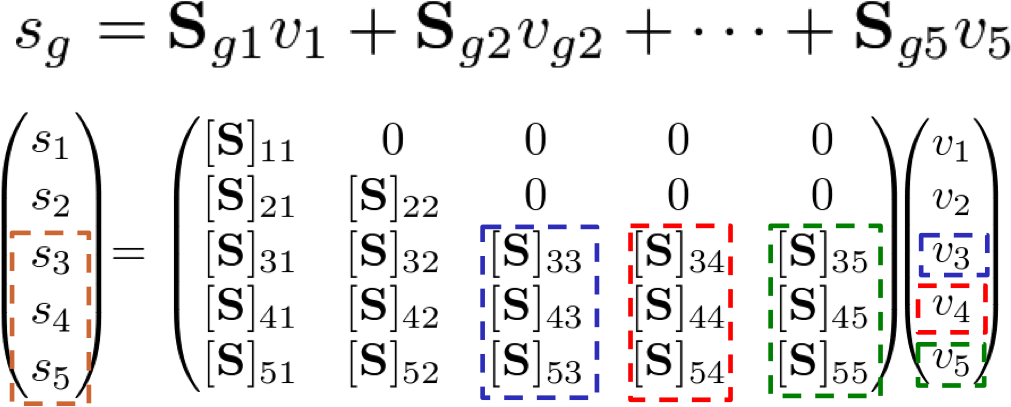
\includegraphics [width=.6\textwidth, height=0.2\textheight ] {KrylovGroupMultiply}
  \end{center}
  \caption{Parallel Implementation of Upscattering Matrix-Vector Multiply}
  \label{fig:KrylovMultiply}
\end{figure}

To implement the energy parallelization, the problem is divided into energy sets, with groups distributed evenly among sets. After each set performs its part of the matrix-vector multiply, a global reduce plus scatter is the only required inter-set communication. Since each set solves the entire spatial mesh with the same spatial decomposition, the established performance of spatial scaling does not change. A picture of the decomposition can be seen in Figure \ref{fig:EnergyDecomp}.
%
\begin{figure}[!h]
  \begin{center}
    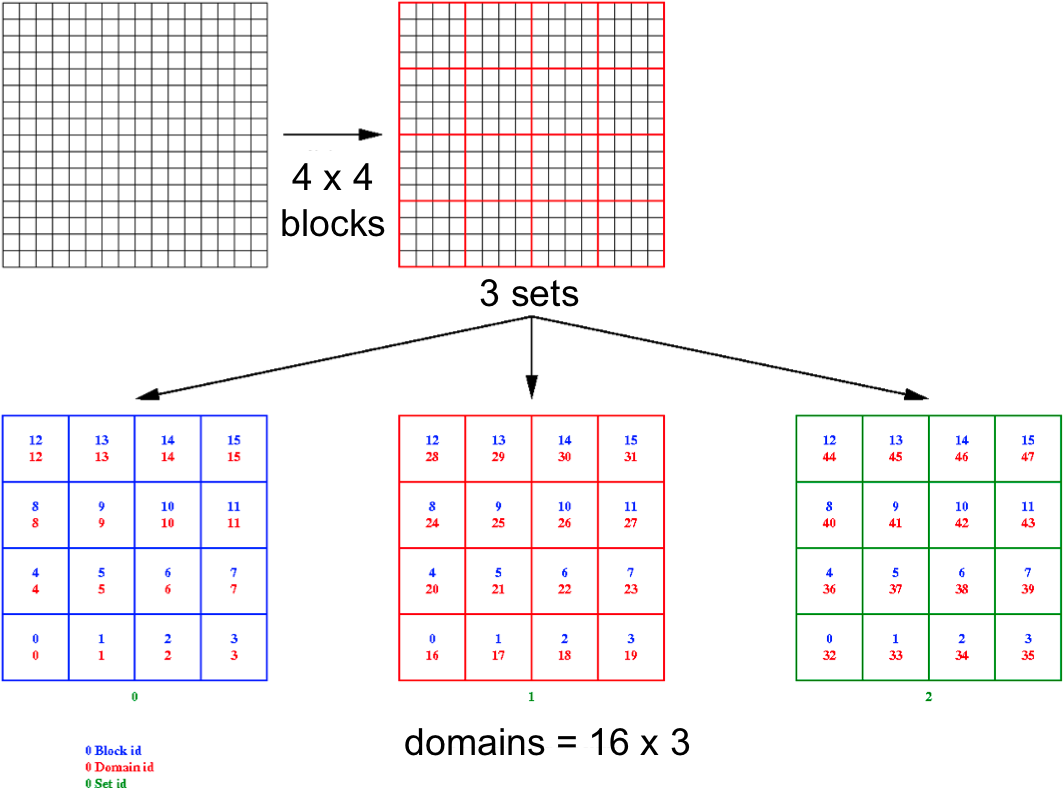
\includegraphics [width=.8\textwidth, height=0.45\textheight ] {EnergySets}
  \end{center}
  \caption{Energy Set Decomposition Added to Denovo \cite{Evans2011}}
  \label{fig:EnergyDecomp}
\end{figure}

It was demonstrated in Section \ref{sec:DenAndPar} that KBA becomes latency dominated when block size becomes small, limiting the number of cores that can be used for a given problem. Energy decomposition offers the ability to further decompose a problem, even after the practical limit of spatial performance for a given mesh has been reached, because scaling can be done across energy instead of space-angle. 

The number of cores is determined by the number of domains. Previously, the number of domains was equal to the number of spatial blocks. Now it is the product of number of energy sets and the number of spatial blocks. For example, with 10,000 spatial blocks (which KBA can handle) and 10 energy sets, Denovo can use 100,000 cores \cite{Evans2011}, \cite{Evans2010}. KBA would not be able to efficiently use 100,000 spatial blocks for meshes of practical interest. This dramatically increases the scalability of Denovo.

Another benefit is having the option to scale in energy rather than space. Once the desired mesh resolution and corresponding spatial decomposition is determined, using finer resolution in energy without energy parallelization makes the problem more costly in terms of both time and memory. To obtain more detailed flux data, fine-grained energy groups are needed. The energy decomposition capability makes this affordable. 

Before this work, no one had decomposed the transport equation in energy nor used one iteration level instead of two. This can now be done because there are machines large enough to store Krylov subspaces made from multiple group-sized iteration vectors, and these computers are large enough to warrant parallelization in energy. 

Note that the Jacobi method could have been used to decompose energy groups before because it is order independent in energy and does not have the large memory footprint associated with Krylov methods. However, there was no need to scale to so many cores and so there was no motivation for this development. Now that the scaling need exists, there is sufficient memory for Krylov methods. Krylov methods are the clear choice because they often converge faster than Jacobi \cite{LeVeque2007}. 

%--------------------------------------------------------------------------------
\subsection{Results}
The new method, which will be referred to as multigroup (MG) Krylov or block Krylov, has been implemented in Denovo. A few test problems were used to investigate the benefits of the new method. One was a small problem intended for initial scoping, and another was a full scale reactor calculation intended for more detailed study. Energy decomposition was investigated from the standpoint of both strong and weak scaling. The problems were also run without energy decomposition, i.e.\ using one energy set, to compare using Krylov instead of GS for the upscatter groups. First MG Krylov and GS are compared, then strong scaling studies are shown, and finally weak scaling is discussed.

\subsubsection{Gauss Seidel vs. Block Krylov}
The small problem was used first to compare GS to MG Krylov for multigroup upscattering. This is a cube of half iron and half graphite discretized with a 50 $\times$ 50 $\times$ 50 orthogonal mesh and decomposed into two spatial domains to use two cores. It is a 27-group problem with 13 upscattering groups and vacuum boundary conditions. An isotropic source is assigned everywhere to all energy groups, and the problem used $P_0$ and $S_4$. The iron plus graphite material composition was chosen for several reasons. Both materials are commonly found in nuclear reactors, graphite is highly scattering and creates a system with a large spectral radius for GS, and the cross sections were available with multiple upscattering groups.

The calculation took $3.51 \times 10^{3}$ seconds using MG Krylov, and the upscattering block converged in 43 GMRES iterations. With GS, the calculation took $2.87 \times 10^{4}$ seconds, or 718\% longer. This case converged in 44 Gauss Seidel iterations, each of which took about 124 GMRES inner iterations, or $\sim$5455 GMRES iterations all together. Note that the Krylov iterations in MG Krylov needed a subspace with a length dimension of 13 energy groups while the Krylov iterations in GS had a length of 1 energy group. This means the cost of the GMRES applications is not the same between solvers. Despite this, GS was very clearly more costly.

A version of this problem with a 10 $\times$ 10 $\times$ 10 grid and an $S_{8}$ angle set was also done. This compared GS, GS accelerated with a two-grid preconditioner (TTG; details are given in Section~\ref{sec:TTG}), and MG Krylov. The solver comparisons can be seen in Table~\ref{table:FeC GS Krylov}. ``GS Iters'' is the number of GS outer iterations and ``Krylov'' is the total number of Krylov iterations needed in the problem. This problem had no spatial or energy decomposition. The MG Krylov solver was faster than both accelerated and unaccelerated GS, and took far fewer Krylov iterations. 
%
\begin{table}[!h]
\caption{Iron Graphite Fixed Source Cube, Multigroup Krylov Compared to Gauss Seidel}
\begin{center}
\begin{tabular}{| l | c | l | c |}
\hline
Solver & GS Iters & Krylov & Time (s)\\[0.5ex]
\hline
GS &  12 & 1,727 & $1.12 \times 10^{2}$ \\
GS TTG & 11 & 1,687 & $1.99 \times 10^{2}$  \\
MG Krylov & n/a & 30 & $8.78 \times 10^{1}$ \\
\hline
\end{tabular}
\end{center}
\label{table:FeC GS Krylov}
\end{table}

Next a more realistic problem, the full-facility PWR core from the Section \ref{sec:DenAndPar}'s weak scaling study, was tested by Evans on the Jaguar machine. This PWR has 289 17 $\times$ 17 assemblies (157 fuel, 132 reflector) and vacuum boundary conditions. There are low, medium, and high enrichment fuel pins. A 2 $\times$ 2 spatial discretization per homogenized fuel pin was used giving 233,858,800 cells. $S_{12}$ was selected as the angular discretization. Two energy groups were used for this test to keep the total problem size small. To get a sense of the problem size, there were 78,576,556,800 unknowns.

It should be noted that Jaguar requires decompositions to be done in a certain way, which determines the number of domains that can be used. For example, keeping the spatial domain size exactly same when changing the number of energy sets is typically not possible so the closest available approximation is chosen instead.

\begin{table}[!h]
\caption{PWR900 with 2 groups, Multigroup Krylov Compared to Gauss Seidel}
\begin{center}
\begin{tabular}{| l | c | c | c | c |}
\hline
Solvers & Blocks & Sets & Domains & Solver Time (m) \\[0.5ex]
\hline
PI + TTG GS & 17,424 & 1 & 17,242 & 11.00 \\
PI + MG Krylov & 10,200 & 2 & 20,400 & 3.03 \\
\hline
\end{tabular}
\end{center}
\label{table:MGkrylovPWR}
\end{table}
%
Table~\ref{table:MGkrylovPWR} shows the results for the PWR900 problem. The goal was to compare MG Krylov and GS using the same number of domains, which required a different spatial decomposition. Power iteration (described in Chapter~\ref{sec:Chp3}) was used as the eigenvalue solver in both cases; GS again used GMRES for the inner iterations and GS was accelerated with TTG. While GS had 15.5\% fewer domains than MG Krylov, it took 263\% longer. Clearly the MG Krylov method was faster than GS for this problem, even when GS was preconditioned and MG Krylov was not. 

In both test cases the new Krylov multigroup solver significantly outperformed Gauss Seidel. The Krylov method took much less time and many fewer iterations, even when Gauss Seidel was accelerated. This demonstrates that the new multigroup solver provides substantial convergence improvement with only space-angle parallelization, which will help solve large and challenging problems. 

\subsubsection{Strong Scaling}
The first two test problems plus an additional system were used to examine strong scaling with energy sets. The iron graphite cube was used first, largely to verify multiset functionality rather than rigorously test scaling. The cube was expanded to a 100 $\times$ 100 $\times$ 100 mesh and decomposed into four spatial blocks to make it large enough to warrant using multisets. It should be noted that it is not expected that this problem will scale particularly well because it is still a small problem and the number of upscattering groups is prime. 

The number of energy sets was varied from 1 to 13. The test problems were run on the small orthanc cluster at ORNL.  The downscattering groups were solved with forward substitution as before, and the upscattering was solved with the Krylov multigroup solver. The upscattering groups converged in 104 GMRES iterations. Every calculation gave the correct flux.

\begin{figure}[!h]
  \begin{center}
    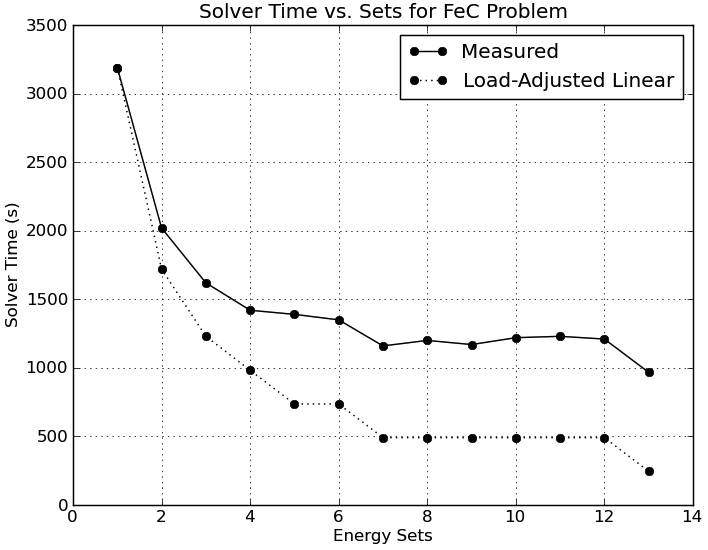
\includegraphics [width=.75\textwidth, height=0.45\textheight ] {FeCKrylovMultisets}
  \end{center}
  \caption{Iron Graphite Fixed Source Cube, Strong Scaling Study}
  \label{fig:FeGraphiteStudy}
\end{figure}
%
Figure~\ref{fig:FeGraphiteStudy} shows the measured time and the ``load-adjusted linear'' time. The perfect, i.e.\ linear scaling, solve time would usually be $(\frac{\text{base\_domains}}{\text{used\_domains}}) \times \text{base\_time}$. However, an alternative method was used to try to account for the load imbalance caused by the energy sets. There is no way to evenly divide 13 groups among energy sets, meaning at least one set always has one more group than the others. The sets with fewer groups must wait for the sets with more groups, which is not an efficient use of processing power. 

To account for the load imbalance, a factor was added that weights the time by the number of groups required for perfect energy load balance divided by the number of groups used. To get this, the maximum number of groups per set was determined, e.g.\ 13 groups / 2 sets = 7 groups. This was multiplied by the number of sets to get the number of groups needed for load balancing, e.g.\ 7 $\times$ 2 = 14. The base case used 4 cores and took $3.19 \times 10^{3}$ seconds. For 2 sets on 8 cores, $t_{\text{linear}} = \frac{4}{8}\times\frac{2\times7}{13} \times (3.19 \times 10^{3}) = 1.72 \times 10^{3}$.

The plotted results lead to a few conclusions. The actual time becomes increasingly different from the ideal time as the number of sets increases until about 5 sets, after which the perfect and measured time are different by an approximately constant amount. Using multisets had a good return on investment for a small number of sets. The efficiency, where efficiency is defined as the ideal time over the observed time, is about 85\% with 2 sets and goes down to about 53\% with 5 sets. Another way to say this is that with 5 sets a speedup of 4.33 would be ideal and a speedup of only 2.30 was observed. 

Overall, this test was not a very good scaling measure because of the load balancing issue. This is illustrated by the fact that the ideal time does not change between 7 sets using 28 cores and and 12 sets using 48 cores. A problem that is not expected to change calculation time when the number of cores increases by 70\% is not a good scaling test. However, this problem did demonstrate that the multiset implementation works, gets the correct answer, and may provide speedup where it makes sense.  

A 44 energy group cross section set was used with the PWR900 to study strong scaling in a more quantitative way than the iron and graphite cube. This many energy groups yielded \\ 1,728,684,249,900 degrees of freedom. Two spatial block - energy set combinations were used, detailed in Table~\ref{table:StrongCasesPWR}. Both cases used power iteration and the MG Krylov solver. Because of the decomposition restrictions, 9,024 spatial domains was the closest available approximation to 10,200.

Some general communication optimization was added to Denovo after these initial results were obtained and the two cases were redone. In Table ~\ref{table:StrongCasesPWR} ``Initial'' is the time taken by the solver before optimization and ``Optimized'' is the time afterwards. The optimization greatly improved the Base case results, reducing the solve time from 49.61 minutes to 38.33 minutes. Unfortunately, there was a negligible difference in the Study case's time. 
%
\begin{table}[!h]
\caption{PWR900 with 44 Groups, Strong Scaling Study}
\begin{center}
\begin{tabular}{| l | c | c | c | c | c |}
\hline
Case & Blocks & Sets & Domains & Initial (m) & Optimized (m) \\[0.5ex]
\hline
Base   & 10,200 & 11 & 112,200 & 49.61 & 38.33 \\
Study & 9,024    & 22 & 198,528 & 34.99 & 34.99 \\
\hline
\end{tabular}
\end{center}
\label{table:StrongCasesPWR}
\end{table}
%
Originally, the perfect time for the Study case was 28.04 minutes, giving an efficiency of 80\%. After optimization, the perfect scaling time became 21.66 minutes, reducing the scaling efficiency to 62\%. All of the data are plotted in Figure~\ref{fig:PWRstrongScaling}. 
\begin{figure}[!h]
  \begin{center}
    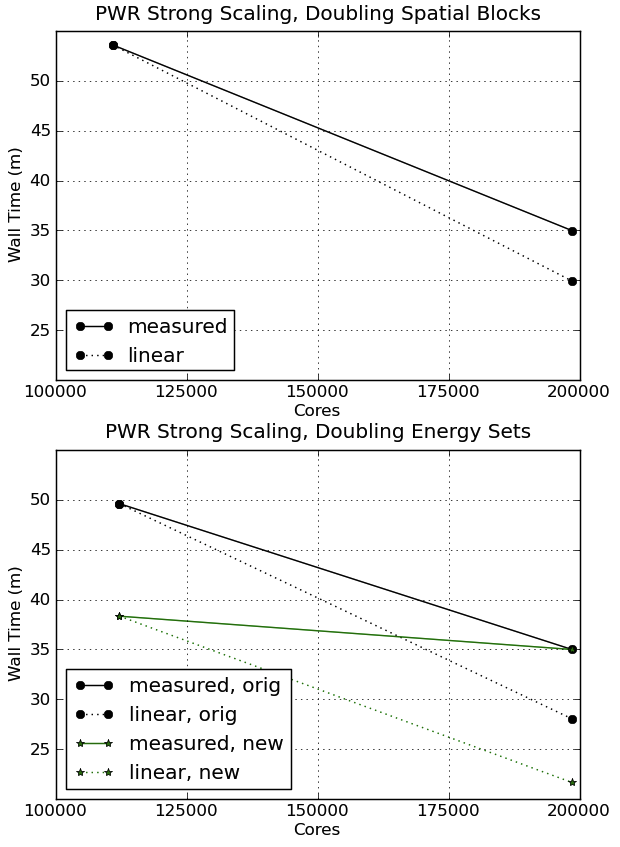
\includegraphics [width=.7\textwidth, height=.45\textheight ] {PWRstrongScaling}
  \end{center}
  \caption{PWR900 with 44 Groups, Strong Scaling Study}
  \label{fig:PWRstrongScaling}
\end{figure}

A variety of reasons have been identified for why the 200,000-core case did not improve as much as the 100,000-core case. Many of these are beyond the scope of this work: it is likely that the problem is not large enough to demonstrate strong scaling well; the block decomposition was not optimal; and there were communication collisions on the torus across the full machine that significantly slowed down communication \cite{Davidson2010}. 

Pertinent to this work, however, is that the multiset communication was not optimal. After each matrix-vector multiply a global reduction and scatter were done. In that process each block on every set got the contribution from every other set, and the data it scattered out was for all groups. The message size for all groups is large and can therefore be slow.

This communication pattern has since been improved by Evans and Davidson to a global reduction followed by a local scatter. When each space-energy domain communicates its updated flux after the multiply, it only communicates to the sets that need its contribution. If the upscattering on one set does not contribute to another set, there is no communication between those sets. The big change, however, is that the data scattered out is only the size of the groups on that set, not all groups \cite{Evans2011b}. In a 44 group problem with 22 sets, that changes the message size from 44-group length to 2-group length. This improvement has been implemented, but the PWR strong scaling calculations have not been repeated. 

To get an idea of the impact of the multiset reduction communication improvement, a fixed source 44 group problem was solved by Davidson with MG Krylov. Three different meshes and spatial decompositions were used for this problem, and each case used a variety of sets. The combinations can be seen in Table~\ref{table:MultisetCommOpt}.
%
\begin{table}[!h]
\caption{Test Cases for Multiset Communication Optimization Study}
\begin{center}
\begin{tabular}{| c | c | l |}
\hline
Mesh & Decomposition & Sets Used \\[0.5ex]
\hline
204 $\times$ 204 $\times$ 90 & 30 $\times$  60 $\times$  2 & 2, 4, 11, 22, 44 \\
408 $\times$ 408 $\times$ 90 & 60 $\times$  72 $\times$  2 & 1, 2, 4, 11, 44 \\
816 $\times$ 816 $\times$ 90 & 120 $\times$  144 $\times$  2 & 1, 2, 4, 11 \\
\hline
\end{tabular}
\end{center}
\label{table:MultisetCommOpt}
\end{table}

To measure the benefit of multiset communication optimization, the percentage of solve time spent doing the reduction across energy sets in the original ``Global Sum'' method is compared to the new ``Reduced Scatter'' method. The results for each mesh - set combination can be seen in Figure~\ref{fig:MultisetCommOpt}. The x-axis is number of energy sets and the y-axis is the percentage of solver time. For example, if the y-value is 3 that means 3\% of the time spent in the solver was used in multiset reduction communication. 
%
\begin{figure}[!h]
  \begin{center}
    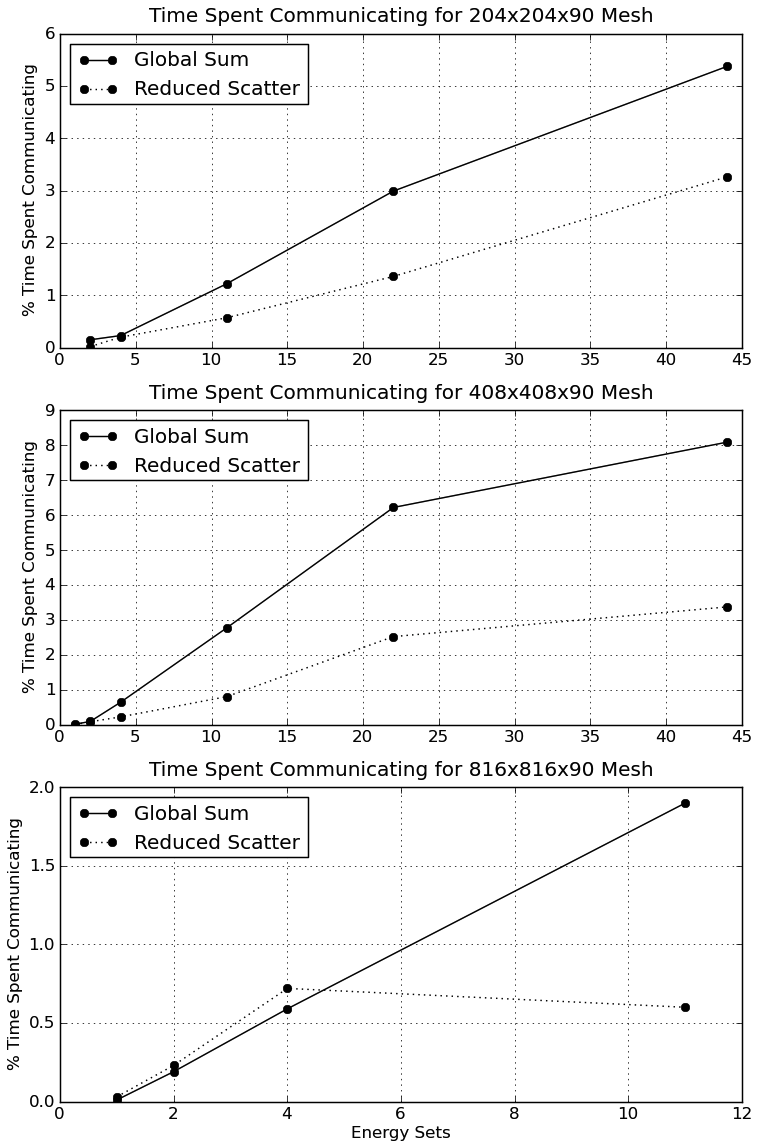
\includegraphics [width=.7\textwidth, height=0.85\textheight ] {MultisetCommOpt}
  \end{center}
  \caption{\% Time Used in Multiset Reduction Communication, Comparison of Old and New Strategies}
  \label{fig:MultisetCommOpt}
\end{figure}

These plots show that in nearly all cases the percentage of time spent on the reduction decreased. As the number of sets increases, the difference in percentage of time also increases. This makes sense because more sets require more reduction communication, so an improved method would have a bigger benefit. However, the spatial decomposition also plays a role since sets communicate across spatial boundaries. The benefit of the new strategy therefore differs for different spatial decompositions. In all cases though, the larger number of sets benefitted from the new implementation. 

These 44 group fixed source tests were also used to study strong scaling when both the general and multiset-specific communication optimizations were in place. These results, which can be seen in Figure~\ref{fig:FxdStrong}, are much better than both the iron graphite cube and PWR900 problems. 
%
\begin{figure}[!h]
  \begin{center}
    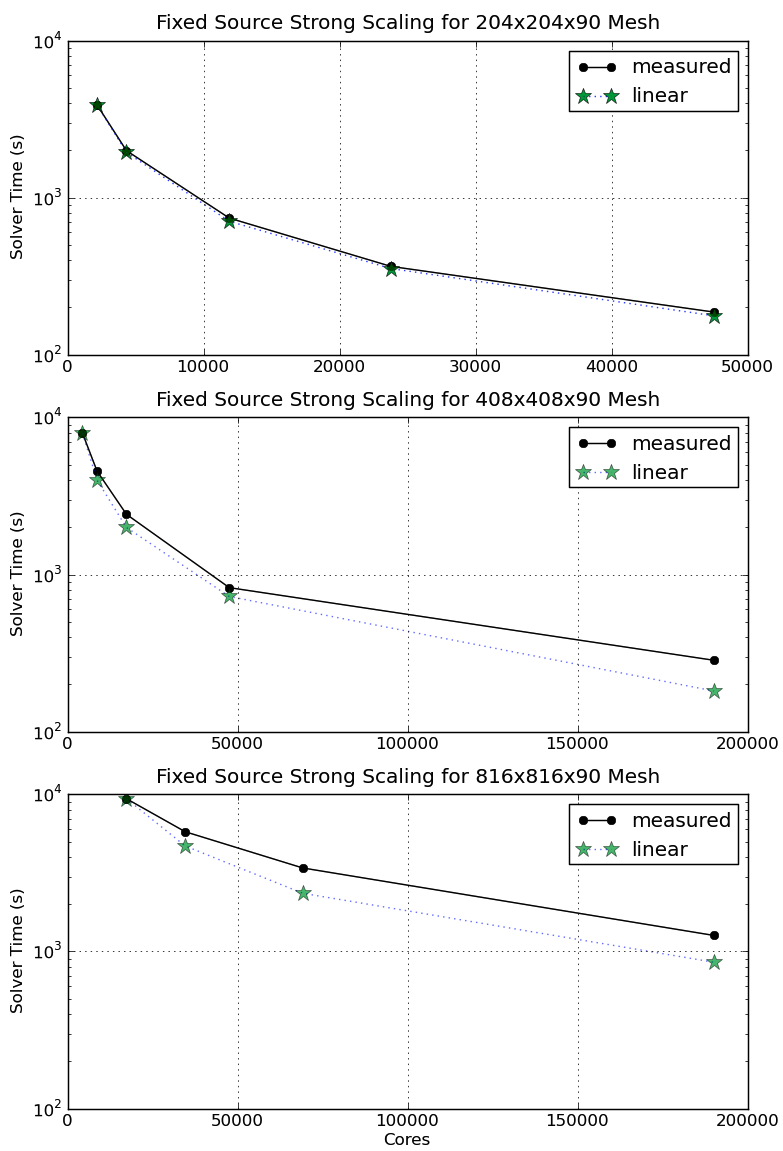
\includegraphics [width=.8\textwidth, height=0.95\textheight ] {FxdSrcKrylovStrongScaling}
  \end{center}
  \caption{Fixed Source Problem with 44 Groups, Strong Scaling Study}
  \label{fig:FxdStrong}
\end{figure}

The first mesh was only large enough for use on up to about 50,000 cores. The 2 set problem was used as the base case for computing linear time. The scaling on this problem was nearly perfect, with an efficiency of 95\% at 47,520 cores and 44 energy sets. 

The scaling was not as close to perfect with the two larger meshes, but it was still much better than the test cases without multiset communication optimization. The medium and large mesh versions both used 1 set as the base case. With the medium sized mesh the efficiency with 47,520 cores and 11 energy sets was 88\%, though the efficiency with 190,080 cores and 44 energy sets was only 64\%. Recall, however, that the PWR case compared 11 and 22 energy sets. If the 44 and 11 set cases are compared, the efficiency increases to 73\%.

The most energy sets used with the largest mesh version was 11. The efficiency with 11 sets on 190,080 cores compared to 1 set and 17,280 cores was 68\%. When comparing the 4 set case that used 69,120 cores to the 11 set case, the efficiency was 98\%, or nearly perfect. 

The 44 group fixed source problem showed that the block Krylov solver can scale fairly well in energy for a variety of spatial discretizations. While strong scaling in energy was not perfect for the medium and large meshes, it was far better than what could be obtained by scaling in space alone for even the largest mesh. The difference between the measured and linear times was not huge compared to the total solution time. 

Further, even when communication was not optimized the multigroup Krylov solver allowed Denovo to solve a real problem with over 1.7 trillion degrees of freedom in under 40 minutes. This problem would not have been practical to solve using the same 233M cell mesh without energy sets, relying on space-angle scaling alone. These results demonstrate that the block Krylov solver allows for the full use of leadership-class machines for problems where KBA would not.

\subsubsection{Weak Scaling}
Finally, the full-facility PWR problem was used for a weak scaling study. The two-group, 17,424-block, GS calculation (PI + TTG GS in Table~\ref{table:MGkrylovPWR}) was compared to the 44-group, 11-set, 10,200-block, MG Krylov calculation with the optimized general communication strategy, but without the multiset communication optimization. 

Recall that there were 78,576,556,800 unknowns when using 2 groups with 1 set on 17,424 cores, and 1,728,684,249,900 unknowns when using 44 groups with 11 sets on 112,200 cores. With weak scaling the problem size/core is typically kept constant. In these tests the problem size/core could not be held constant, so an adjustment factor was included. The number of energy groups were used to weight the problem size/core and that was used to get an adjusted solve time of 11.21 minutes for the MG Krylov calculation: $[(\frac{44}{2})(\frac{17,424}{112,200})]^{-1}\times38.33$ = 11.21. 

Efficiency for weak scaling is calculated by taking the ratio of the MG Krylov adjusted time to the reference time, or 11.21 over 11.00, giving an efficiency of 1.019. A plot of the weak scaling is shown in Figure~\ref{fig:PWRweakScaling}. Note that perfect weak scaling would maintain an efficiency of 1, thus the weak scaling observed here was very good. Recall that a weak scaling study using this same problem was reported in Section~\ref{sec:DenAndPar}. The performance with energy sets was markedly better than with KBA alone, showing that energy decomposition can improve weak scaling.
%
\begin{figure}[!h]
  \begin{center}
    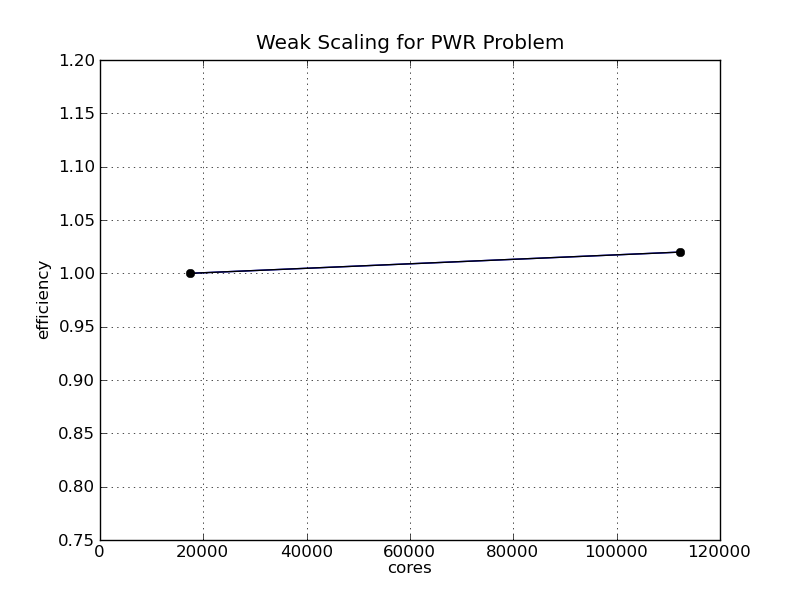
\includegraphics [width=.8\textwidth, height=0.48\textheight ] {PWRmyWeakScaling}
  \end{center}
  \caption{PWR900, Weak Scaling Study}
  \label{fig:PWRweakScaling}
\end{figure}

%-----------------------------------------------------
\subsection{Implications}
The tests just discussed show that the multigroup Krylov solver provides a time benefit both from using a Krylov solver for the equivalent of the outer iterations instead of Gauss Seidel and from the parallelization in energy that is enabled by this method. There were no deterministic transport codes found that decompose the upscatter calculation in energy, nor that only use one iteration level for the upscattering block. This decomposition is a new contribution to the field and helps alleviate the scaling limitations associated with KBA.   

There are a few reasons this has not been pursued before, primarily based on computer architecture and existing code capability. Memory has only become large enough to accommodate the necessary Krylov subspaces recently. Only in the last several years have there been computers with enough processing capability to allow for scaling to hundreds of thousands of cores, motivating energy decomposition. In addition, the inner-outer paradigm is at the core of most transport codes and in many cases it would take substantial effort to modify that structure. 

Note that an explicit block Jacobi method, which converges more slowly than GS by a factor of two, could have been used previously to decompose energy groups because it is explicit in energy and does not have the large memory footprint associated with Krylov methods. However, there was no need to scale to so many cores and so there was no motivation for this development. Now that the scaling need exists, there is sufficient memory for Krylov methods. Krylov methods are the clear choice because they often converge faster than Jacobi \cite{LeVeque2007}. 

Transport codes could have used machines with hundreds of thousands of cores without energy parallelization by solving problems with extremely large meshes. Doing this, though, would typically involve refining a problem's mesh for the sake of refining its mesh and not because the quality of solution requires more spatial resolution. In addition, this strategy does not address the need for increased energy resolution while decomposing in energy does. 

Overall, the tests showed the multigroup Krylov solver decisively accomplishes the goal of accelerating transport calculations by using new computers fully. The first two test problems illustrated that the block Krylov method does the multigroup iterations more quickly than the Gauss Seidel method. The strong scaling studies showed that the energy decomposition works and the method provides reasonably good strong scaling in energy. The weak scaling study showed that the MG Krylov method weak-scaled better than GS with only space-angle decomposition. 

\separatorpage{}
              % Chapter 2, ``Krylov for upscattering''
 % Prelim, Chapter 3
% by Rachel Slaybaugh

\chapter{Eigenvalue Acceleration}
\label{sec:Chp3}
Nuclear engineers are often concerned with finding the criticality state of a reactor. The term critical means that the fission chain reaction is self-sustaining, i.e.\ every neutron produces one new neutron. In the context of Equation~\ref{eq:neutron transport}, this corresponds to $k = 1$. If $k < 1$, the reaction is subcritical and the total number of neutrons decreases over time. If $k > 1$, the reaction is supercritical and the total number of neutrons increases over time \cite{Duderstadt1976}. Steady-state reactor behavior is generally the operation mode of interest, and the typical concern is only the dominant eigenmode. The remaining eigenvalues can describe regional instabilities and may be useful for some analysis goals \cite{Vidal1998}. 

The ability to quickly and accurately determine the state of a multiplying nuclear system is very important in designing new nuclear systems. The standard eigenvalue solution methods can be slow for some cases of interest. To design new reactors, better solvers are needed. This chapter discusses the new eigenvalue solver that has been implemented to meet this challenge. Some background about eigenvalue solution methods is presented first. These methods are then put into the context of what has been done in the past and are used to explain how the new method works and why it is novel. Finally, results from the new solver are presented.

%-----------------------------------------------------------------------------------------
\section{Background}
Details about eigenvalue problems, characteristics of convergence, and eigenvalue solution methods are all needed to understand the new eigenvalue solver. The generalized eigenvalue problem takes the form $\ve{B}x = \mu \ve{C}x$ and can be transformed into an ordinary eigenvalue problem, $\ve{A}x = \lambda x$. Both forms have the same right eigenvectors. If $\ve{C}$ is non-singular then $\ve{A} = \ve{C}^{-1}\ve{B}$ and then the problem $v = \ve{A}x$ can be solved in two steps: \cite{Stewart2001}
%
\begin{enumerate}
  \item $w = \ve{B}x$
  \item Solve the system $\ve{C}v = w$.
\end{enumerate}
%
Because the generalized form can be converted to the ordinary form, this chapter will focus on the ordinary form without loss of applicability.

Some basic notation will be needed: let $\sigma(\ve{A}) \equiv \{\lambda \in \mathbb{C} : rank(\ve{A} - \lambda \ve{I}) \le n\}$ be the spectrum of $\ve{A}$, where the elements in the set are the eigenvalues and $\mathbb{C}$ is the set of complex numbers. The eigenvalues can be characterized as the $n$ roots of the polynomial $p_{\ve{A}}(\lambda) \equiv det(\lambda \ve{I} - \ve{A})$. Each distinct eigenvalue in $\sigma(\ve{A})$ has a corresponding nonzero vector $x$ such that $\ve{A}x_{i} = \lambda_{i} x_{i}$ for $i = 1,...,n$ \cite{Sorensen1996}. It will be assumed that the eigenvalues are ordered as $|\lambda_{1}| > |\lambda_{2}| \ge \dots \ge |\lambda_{n}| \ge 0$. 

Eigenvalue problems in the nuclear transport community are typically solved with iterative rather than direct methods. A variety of iterative solvers have been used to solve eigenvalue problems. This subsection will cover the methods that have been most widely used in the nuclear field as well as methods that will aid in understanding the work being proposed. 

%-----------------------------------------------------------------------------------------
\subsection{Convergence Concerns}
Before the methods are discussed, some terms that are used to characterize how numerical methods might behave when solving problems of interest are presented. A method's behavior can be affected by characteristics of the mathematical problem ($f : X \to Y$) as well as by characterisitics of the algorithm itself ($\tilde f : X \to Y$). The material in this subsection is derived from Trefethen and Bau \cite{Trefethen1997}; see this reference for more detail.

Conditioning is one way to express the perturbation behavior of the mathematical problem. A \emph{well-conditioned} problem is one in which all small perturbations of $x$ lead to only small changes in $f(x)$. An \emph{ill-conditioned} problem is one in which some small perturbation of $x$ leads to a large change in $f(x)$. The condition number is a quantity used to express how well-conditioned a matrix or problem is. A small condition number corresponds to a well-conditioned problem, and vice versa. 

The relative condition number is used to measure the effect of relative perturbations. This is particularly useful in numerical analysis because computers introduce relative errors. Let $\delta x$ be a small perturbation of $x$ and $\delta f = f(x + \delta x) - f(x)$. With these terms, the relative condition number is defined as
%
\begin{equation}
  \kappa(x) = \lim_{\delta \rightarrow 0} \sup_{||\delta x|| \le \delta} \biggl(\frac{||\delta f||}{||f(x)||} / \frac{||\delta x||}{||x||} \biggr)  \:,
  \label{eq:cond}
\end{equation}
%
where $\sup$ is the supremum, the smallest real number that is greater than or equal to every number in the set in question \cite{Wikipedia2011}. This definition holds for any norm. To express a specific norm, a sub number will be added, e.g.\ the two norm would be indicated by $\kappa_{2}(x)$.

The condition number of a matrix $\mathbf{A}$ is defined as
%
\begin{equation}
  \kappa(\mathbf{A}) = ||\mathbf{A}|| \text{ }||\mathbf{A}^{-1}|| \:.
  \label{eq:condA}
\end{equation}
%
If $\mathbf{A}$ is singular, its condition number is infinity. If the two-norm is used, then $||\mathbf{A}|| = \sigma_{1}$, $||\mathbf{A}^{-1}|| = \sigma_{m}$, and $\kappa_{2}(\mathbf{A}) = \frac{\sigma_{1}}{\sigma_{m}}$. Here $\sigma_{j}$ is the $j$th singular value of $\mathbf{A}$, and the singular values are ordered such that $\sigma_{1} \ge \sigma_{2} \ge \dots \ge \sigma_{n} > 0$. The ratio $\frac{\sigma_{1}}{\sigma_{m}}$ can be interpreted as the eccentricity of the hyper-ellipse that is the image of an $m$-dimensional unit sphere under $\mathbf{A}$. When $\ve{A}$ has a large condition number the largest principle semiaxis is much longer than the smallest principle semiaxis. 

Stability is a way to express the perturbation behavior of an algorithm used to solve a problem on a computer. A stable algorithm ``gives nearly the right answer to nearly the right question.'' An algorithm $\tilde f$ for a problem $f$ is stable if each $x \in X$ satisfies
\begin{equation}
  \frac{||\tilde f(x) - f(\tilde x)||}{||f(\tilde x)||} = O(\epsilon_{machine}) \qquad \text{for some } \tilde{x} \text{ with } \frac{||\tilde x - x||}{||x||} = O(\epsilon_{machine}) \:.
  \label{eq:stable}
\end{equation}

Backwards stability has a tighter requirement than stability alone, and a backwards-stable algorithm will ``give exactly the right answer to nearly the right question.'' An algorithm $\tilde{f}$ for a problem $f$ is backwards stable if, for each $x \in X$,
%
\begin{equation}
  \tilde{f}(x) = f(\tilde{x}) \qquad \text{for some } \tilde{x} \text{ with } \frac{||\tilde{x} - x||}{||x||} = O(\epsilon _{machine}) \:.
  \label{eq:back stable}
\end{equation}

The concepts of condition and stability are not independent of one another. The accuracy of a backwards stable algorithm depends on the condition number, $\kappa(x)$ of $f$. The relative errors of an algorithm applied to some problem satisfy:
%
\begin{equation}
  \frac{||\tilde{f}(x) - f(x)||}{||f(x)||} = O(\kappa(x) \epsilon _{machine}) \:.
\end{equation}
These ideas and definitions will be needed when considering the behavior of the new eigenvalue solver in combination with the multigroup Krylov solver. 

%-----------------------------------------------------------------------------------------
\subsection{Power Iteration}
Power iteration (PI) is an old and straightforward algorithm for finding an eigenvalue/vector pair. The basic idea is that any nonzero vector can be written as a linear combination of the eigenvectors of $\ve{A}$ because the eigenvectors are linearly independent, namely $v_0 = \gamma_1 x_1 + \gamma_2 x_2 + \cdots + \gamma_n x_n$ where $x_{j}$ is the $j$th eigenvector and $\gamma_{j}$ is some constant. This specific expression assumes a non-defective $\ve{A}$, though this assumption is not necessary for the method to work. 

Another fact that is used to understand power iteration is that $\ve{A}^k x_i = \lambda_i^k x_i$. Thus
%
\begin{equation}
  \ve{A}^k v_{0} = \gamma_1 \lambda_1^k x_1 + \gamma_2 \lambda_2^k x_2 + \cdots + \gamma_n \lambda_n^k x_n \:.
  \label{eq:Ak}
\end{equation}
%
Since $|\lambda_1| > |\lambda_i|, i \ne 1$, the first term in the expansion will dominate as $k \to \infty$ and $\ve{A}^k v_{0}$ therefore becomes an increasingly accurate approximation to $x_1$. In practice, it is desirable to avoid exponentiating a matrix and it is helpful to normalize $v$ in order to avoid possible over or underflow. This leads to Algorithm \ref{algo:PI} \cite{Stewart2001}. 
%
\begin{algorithm}
  Given $\ve{A}$ and $v_0$, $v = \frac{v_{0}}{||v_{0}||_{\infty}}$. \\
  Until convergence do:
  \begin{list}{}{\hspace{2em}}
    \item $w = \ve{A}v$
    \item $\lambda = \frac{w^{T}v}{v^{T}v}$
    \item $i = i_{max}(w)$
    \item $v = \frac{v}{e_{i}^{T}w}$.
  \end{list}
  \caption{Power Iteration}
  \label{algo:PI}
\end{algorithm}

Using Equation \eqref{eq:Ak} and Algorithm \ref{algo:PI} it is easy to understand PI's convergence behavior. After $k$ steps, the iteration vector will be: 
%
\begin{equation}
  v_{k} = \bigl( \frac{\lambda_{1}^{k}}{e_{i}^{T}\ve{A}^{k}v_{0}} \bigr) \bigl(\frac{1}{\lambda_{1}^{k}}\ve{A}^{k}v_{0} \bigr) \:.
\end{equation}
% 
If $\ve{A}$ has eigenpairs $\{(x_{j}, \lambda_{j}), 1 \le j \le n \}$ and $v_{0}$ has the expansion $v_{0} = \sum_{j=1}^{n} x_{j}\gamma_{j}$ then
%
\begin{equation}
  \frac{1}{\lambda_{1}^{k}}\ve{A}^{k}v_{0} =  \frac{1}{\lambda_{1}^{k}} \sum_{j=1}^{n} \ve{A}^{k}x_{j}\gamma_{j} = \sum_{j=1}^{n} x_{j} \bigl(\frac{\lambda_{j}}{\lambda_{1}} \bigr) \gamma_{j} \:.
  \label{eq:PIexpand}
\end{equation}
%
Equation \eqref{eq:PIexpand} shows that this algorithm converges at the linear rate of $|\frac{\lambda_{2}}{\lambda_{1}}|$, which is called the dominance ratio. If $\lambda_2$ is close to $\lambda_1$, then this ratio will be close to unity and the method will converge very slowly. If $\lambda_2$ is far from $\lambda_1$, then convergence will happen much more quickly. Put simply, PI is better suited for problems where $\ve{A}$ has eigenvalues that are well separated \cite{Sorensen1996}.  

Power iteration is very attractive because it only requires matrix-vector products and two vectors of storage space. Because of its simplicity and low storage cost, PI has been widely used in the transport community for criticality problems for quite some time \cite{Lewis1993}, \cite{Warsa2004a}. Despite these beneficial characteristics many current codes use an acceleration method with PI, or have moved away from it altogether because of the slow convergence for many problems of interest. Nevertheless it is still used in some codes, has historical relevance, and is used in many studies as a base comparison case. 

As an aside, it is interesting to point out the connection between Krylov methods and power iteration. The power method is a Krylov method that uses a subspace of dimension one.  A Krylov subspace is built by storing the vectors created during each iteration of the power method. Krylov methods with subspaces larger than one take advantage of the information generated during each iteration that the power method discards. 

%-----------------------------------------------------------------------------------------
\subsection{Shifted Inverse Iteration}
One way to improve power iteration is to shift the matrix $\ve{A}$ and then, in a power iteration-type scheme, apply the inverse of the shifted matrix rather than the regular unshifted matrix. The method is called shifted inverse iteration and the goal is to provide better convergence properties. Understanding why shifted inverse iteration is an improvement requires understanding spectral transformation. 

The fundamental notion is that $\ve{A}$ can be shifted by a scalar without changing the eigenvectors. That is, for some shift $\mu$, $(\ve{A} - \mu \ve{I})$ will have the same eigenvectors as $\ve{A}$ \cite{Sorensen1996}. If $\mu \notin \sigma(\ve{A})$, then $(\ve{A} - \mu \ve{I})$ is invertible and $\sigma([\ve{A} - \mu \ve{I}]^{-1}) = \{1/(\lambda - \mu):\lambda \in \sigma(\ve{A})\}$. Eigenvalues of $\ve{A}$ that are near the shift will be transformed to extremal eigenvalues that are well separated from the others. Such a spectral transformation can be added to the power method. Given an estimate, $\mu \approx \lambda_1$, the shifted inverse power method will usually converge more quickly than PI.

To see why this works consider: 
%
\begin{equation}
    \tau_1 = \frac{1}{\lambda_1 - \mu}\text{ , }\tau_2 = \frac{1}{\lambda_2 - \mu}\text{ , }\dots\text{ , }\tau_n = \frac{1}{\lambda_n - \mu} \:.
\end{equation}
%
As $\mu \to \lambda_1$, $\tau_1 \to \infty$ and all the other eigenvalues go to finite quantities. If the $\tau$s are inserted into the convergence analysis done for PI, it can be shown that the inverse power method will converge as $\frac{|\lambda_{1} - \mu|}{|\lambda_{2} - \mu|}$. This is typically much faster than $|\frac{\lambda_{2}}{\lambda_{1}}|$, though the ultimate success of the method is dependent upon the quality of the shift \cite{Sorensen1996}, \cite{Trefethen1997}. 

The algorithm for shifted inverse iteration is much like that for power iteration, requiring only a few simple changes. Step 1 now becomes ``solve $(\ve{A}-\mu \ve{I})w = v$'' and Step 3 becomes $\lambda = \mu + \frac{w^{T}v}{w^{T}w}$; all other steps are the same. After convergence, the actual eigenvalue of interest is backed out using the eigenvector \cite{Sorensen1996}.  Shifted inverse iteration is identical to performing power iteration on $(\ve{A}-\mu \ve{I})^{-1}$. 

On initial consideration it would seem shifted inverse methods might not work well when the shift is very good because the matrix becomes very ill-conditioned. If the shift is exact, i.e.\ when $\mu = \lambda_{1}$, the matrix is singular. It turns out this concern is unfounded. Peters and Wilkinson proved that ill-conditioning is not a problem for inverse iteration methods \cite{Peters1979}. Trefethen and Bau also assert that this is the case as long as the $\ve{A}w = v$ portion is solved with a backwards stable algorithm \cite{Trefethen1997}.

Wielandt's method is a flavor of shifted inverse iteration that has been used widely in the neutron transport community, though it was originally developed in 1944 in an unrelated context \cite{Zinzani2008}, \cite{Itagaki1996}, \cite{Itagaki2002}, \cite{Ipsen}. In the transport equation formulation, Wielandt's method changes the eigenvalue problem from $\ve{A}\phi = \gamma \ve{F} \phi$ to $(\ve{A} - \gamma_e \ve{F})\phi = \delta \gamma \ve{F} \phi$ where $\gamma_e$ is an estimate for $\gamma_1$ and $\delta \gamma = \gamma_1 - \gamma_e$. This is formulated as a generalized eigenvalue problem and the eigenpair is $(\phi, \gamma)$, where $\gamma = \frac{1}{k}$.

The power method with iteration index $k$ is applied to the system, giving $\phi^k = \delta \gamma^{k-1}(\ve{A} - \gamma_e \ve{F})^{-1}\ve{F}\phi^{k-1}$. The estimate, $\gamma_e$, can be improved on each iteration by starting with an initial guess of $0$ and setting $\gamma_e^k = \delta \gamma^{k-1} + \gamma_e^{k-1} + \alpha$. Here $\alpha$ is an optional small positive constant that is designed to keep roundoff error from dominating when $\gamma_e$ becomes very close to $\gamma_1$ \cite{Nakamura1977}. 

Studies of reactor systems have found shifted inverse iteration to be faster than power iteration \cite{Allen2002}. In the general computational community, shifted inverse iteration has largely taken the place of power iteration when looking for eigenvectors associated with eigenvalues that are relatively well known at the outset of the calculation since this information allows for the selection of a good shift \cite{Ipsen}.  

%-----------------------------------------------------------------------------------------
\subsection{Rayleigh Quotient Iteration}
Rayleigh quotient iteration is a variation of shifted inverse iteration that has a changing shift like Wielandt's method sometimes does. The key difference is that this method uses a specific formula, the Rayleigh quotient (RQ), that is designed to find the optimal the shift at every iteration. 

The Rayleigh quotient for the ordinary eigenvalue problem, originally proposed by the third Baron Rayleigh in the 1870s, is defined as \cite{Parlett1974}:
%
\begin{equation}
  \rho(x) = \frac{x^{T}\ve{A}x}{x^{T}x} \:.
  \label{RQ}
\end{equation}
%
If $x$ is an eigenvector of $\ve{A}$, then the RQ is the corresponding eigenvalue. If $x$ is close to an eigenvector, then the RQ will approximate the eigenvalue \cite{Stewart2001}. The derivation of the RQ comes from asking the question ``what $\alpha$ will minimize $||\ve{A}x - \alpha x||_2$?'' Solving this using least squares will give $\alpha = \rho(x)$ \cite{Trefethen1997}. 

The RQ has a similar form for the generalized eigenvalue problem, mentioned here because it applies to some of the past work discussed below and is the form that was implemented in the new solver. For the problem $\ve{A}x = \lambda \ve{B}x$, there is a right eigenpair $(\lambda, x)$ for $x \ne 0$ and a left eigenpair $(\lambda, y): y^{T}\ve{A} = \lambda y^{T}\ve{B}$ for $y \ne 0$, of the pencil $(\ve{A}, \ve{B})$. Let $\langle \alpha, \beta \rangle$ be a simple eigenvalue of pencil $(\ve{A}, \ve{B})$. If $x$ and $y$ are right and left eigenvectors corresponding to $\langle \alpha, \beta \rangle$, respectively, then $\langle \alpha, \beta \rangle = \langle y^{T} \ve{A} x, y^{T} \ve{B} x \rangle$. This means the ordinary form of the eigenvalue is:
\begin{equation}
 \lambda = \frac{y^{T} \ve{A} x}{y^{T} \ve{B} x} \:,
\end{equation}
which is the generalization of the RQ \cite{Stewart2001}. 

Recall from the previous subsection that choosing a shift close to the eigenvalue of interest controls the dominance ratio of shifted inverse iteration, and hence convergence. The RQI algorithm simply uses a strategically selected shift; see Algorithm \ref{algo:RQI}.
\begin{algorithm}
  Choose a starting unit vector, $v_{0}$, then for $k = 0,1,2,\dots$
  \begin{list}{}{\hspace{2.5em}}
    \item form $\rho_{k} = \rho(v_{k}) = v_{k}^{T}\ve{A}v_{k}$,
    \item if $\ve{A} - \rho_{k}$ is singular, then solve $(\ve{A} - \rho_{k})v_{k+1} = 0$ for $v_{k+1} \ne 0$ and halt. Otherwise 
    \item solve $(\ve{A} - \rho_{k})w_{k+1} = v_{k}$,
    \item normalize $v_{k+1} = \frac{w_{k+1}}{||w_{k+1}||}$.
  \end{list}
  \caption{Rayleigh Quotient Iteration}
  \label{algo:RQI}
\end{algorithm}
%
This process generates a sequence, $\{\rho_{k}, v_{k}\}$, called the Rayleigh sequence generated by $v_{0}$ on $\ve{A}$. To more deeply understand why this method is optimal and useful for the purposes of this work, more properties of the Rayleigh quotient must highlighted \cite{Parlett1974}: 
%
\begin{itemize}
  \item For $\alpha \ne 0$, $\rho(\alpha x, \ve{A}) = \rho(x, \ve{A})$, so using any multiple of $x$ will produce the same sequence as $x$. 
  \item The RQ has translational invariance, $\rho(x, \ve{A} - \alpha \ve{I}) = \rho(x,\ve{A}) - \alpha$, meaning the matrix $(\ve{A} - \alpha \ve{I})$ produces the same sequence as $\ve{A}$ \cite{Parlett1974}. This relationship can be used to relate eigenvalues and applied shifts. In fact, this is one of the ways to find the eigenvalue of interest for the standard inverse iteration method \cite{Sorensen1996}. 
\item When $x$ is an eigenvector of $\ve{A}$, $\rho(x)$ is stationary at $x$.  
\item When $x \ne 0$ the RQ gives the minimal residual, with equivalence holding only when $\beta = \rho(x)$:
%
\begin{equation}
  ||(\ve{A} - \beta)x||^{2} \le ||\ve{A}x||^{2} - ||\rho(x)x||^{2} \:.
\end{equation}
%
\item A corollary of this is that $x$ is orthogonal to $(\ve{A} - \rho(x))x$ \cite{Parlett1974}. 
\end{itemize}

RQI has very good convergence properties for normal matrices. The minimal residual property of the RQ causes good global convergence behavior. The sequence of residuals $\{ ||(\ve{A} - \rho_{k})v_{k}|| = ||r_{k}||, k = 0, 1, ... \}$ is monotone decreasing for all starting $v_{0}$. When RQI is applied to normal matrices, the following has been proven as $k \to \infty$:
%
\begin{enumerate}
 \item $\rho_{k} = \rho(v_{k})$ converges, and either
 \item $(\rho_{k}, v_{k})$ converges cubically to an eigenpair $(\lambda, k)$, or
 \item $\rho_{k}$ converges linearly to a point equidistant from $s \ge 2$ eigenvalues of $\ve{A}$, and the sequence $\{v_{k}\}$ cannot converge. 
\end{enumerate}
%
This means that when RQI converges to the correct eigenpair it does so rapidly. However, there is a risk that if a bad starting vector is selected it will not converge at all. 

The monotone sequence $\{||r_{k}||\}$ is bounded from below by 0. If the limit of the sequence is 0 as $k \to \infty$ then case 2 will be observed and convergence will be cubic. If the limit is greater than 0, case 3 is found. Unfortunately, it does not seem that this can be know a priori. In practice, however, users found that it was difficult to make the method fail for normal matrices \cite{Parlett1974}. 

For non-normal matrices the stationary property does not hold, which means the convergence is quadratic at best. The residual sequence is also not guaranteed to be monotone decreasing and thus no global convergence properties can be proven. It has been found in practice that RQI will still converge for non-normal systems, just at a slower rate than for normal matrices. However, convergence cannot be guaranteed nor predicted in advance \cite{Parlett1974}. 

%To deal with this, two adapted RQI methods for non-normal matrices were developed that attempt rectify this. One developed Ostrowski regains the stationary property at eigenvectors. In the non-defective case this gives cubic convergence, but gives no guarantees of global convergence. The other was developed by Parlett and it generates monotonically decreasing residuals, thus guaranteeing global convergence but at a rate that is merely linear for non-defective matrices \cite{Parlett1974}. 

%-----------------------------------------------------------------------------------------
\subsection{Krylov Methods}
The multigroup Krylov solver is used over all energy groups inside the new eigenvalue solver. Because this requires applying a Krylov method to a shifted system, some additional facts about Krylov methods are needed. Krylov subspaces have the property that for any $\mu$, $\mathcal{K}_k(\ve{A},x) = \mathcal{K}_k(\ve{A}- \mu \ve{I}, x)$. This means that a Krylov method can be applied to a shifted system and the correct eigenvector will still be found \cite{Stewart2001}. 

Convergence and stability properties differ from Krylov method to Krylov method. Because GMRES is the most widely used Krylov method in this work, convergence and stability discussions will focus on this method. Paige et.\ at.\  \cite{Paige2006} demonstrate that the least squares solution at every step in GMRES is always backwards stable. GMRES is also backwards stable when finding $x$ in $\ve{A}x = b$ for ``sufficiently nonsingluar $\ve{A}$.'' An $n \times n$ $\ve{A}$ that qualifies as nonsingular enough satisfies
%
\begin{equation}
  \ve{A}x = b \ne 0\:, \qquad \ve{A} \in \mathbb{R}^{n \times n} \:, \qquad b\in \mathbb{R}^{n} \:, \qquad \sigma_{min}(\ve{A}) \gg n^{2}\epsilon ||\ve{A}||_{F} \:.
\end{equation}
%
Here $\epsilon$ is the floating point arithmetic unit roundoff, $|| \cdot ||_{F}$ is the Frobenius norm, and $\sigma_{min}(\ve{A})$ is the minimum singular value of $\ve{A}$. Using the notation that $\ve{\tilde V}_{m}$ is the $n \times m$ orthonormal matrix computed at step $m$ of the modified Gram-Schmidt procedure during the Arnoldi process and includes rounding error, GMRES is also backwards stable up until  \cite{Paige2006}
%
\begin{equation}
  \kappa_{2}(\ve{\tilde V}_{m}) = \frac{\sigma_{max}(\ve{\tilde V}_{m})}{\sigma_{min}(\ve{\tilde V}_{m})} \le \frac{4}{3} \:.
\end{equation}

Trefethen and Bau \cite{Trefethen1997} point out that evaluation of the convergence properties of GMRES is facilitated by relating it to a polynomial approximation problem. GMRES solves this approximation problem: find $p_{n} \in P_{n}$ such that 
%
\begin{align}
  ||p_{n}(\ve{A})b||_{2} &= \text{minimum,} \qquad \text{where}  \nonumber \\
  P_{n} &= \{ \text{polynomials } p \text{ of degree } \le n \text{ with } p(0)=1 \nonumber \}.
\end{align}
%
This polynomial requires the first coefficient to be 1, which is a normalization at $z=0$ . GMRES chooses the coefficients of the polynomial $p_{n}$ to minimize the norm of the residual, $r_{n} = b - \ve{A}x_{n} = (\ve{I} - \ve{A}q_{n} (\ve{A}) )b$; $q_{n}$ is a polynomial of degree $n-1$ and $p_{n}(z) = 1 - zq(z)$ \cite{Trefethen1997}.

GMRES is monotonically convergent: $||r_{n+1}||_{2} \le ||r_{n}||_{2}$. In addition, $||r_{n}||_{2} = ||p_{n}(\ve{A})b||_{2} \le ||p_{n}(\ve{A})||_{2}$ $||b||_{2}$. Thus, the convergence rate of GMRES is determined by
%
\begin{equation}
  \frac{||r_{n}||_{2}}{||b||_{2}} \le \inf_{p_{n}\in P_{n}} ||p_{n}(\ve{A})||_{2} \:.
\end{equation}
%
To get an idea of how quickly GMRES can converge, the question of how small $||p_{n}(\ve{A})||$ can be for a given $n$ and $\ve{A}$ must be answered. For this analysis let $\ve{A}$ be diagonalizable such that $\ve{A}=\ve{V} \Lambda \ve{V}^{-1}$, where $\Lambda = \Lambda(\ve{A})$ is a diagonal matrix of eigenvalues for $\ve{A}$ and $\ve{V}$ is a non-singular matrix of eigenvectors. Also define the scalar $||p||_{S} = \sup_{z\in S} |p(z)|$. Then \cite{Trefethen1997}
%
\begin{equation}
  ||p(\ve{A})||_{2} \le ||\ve{V}||_{2} \text{ } ||p(\Lambda)||_{2} \text{ } ||\ve{V}^{-1}||_{2} = \kappa_{2}(\ve{V}) ||p||_{\Lambda(\ve{A})} \:.
\end{equation}

All of this can be combined to say that at step $n$ of GMRES, the residual satisfies
%
\begin{equation}
  \frac{||r_{n}||_{2}}{||b||_{2}} \le \kappa_{2}(\ve{V})  \inf_{p_{n}\in P_{n}} ||p||_{\Lambda(\ve{A})} \:.
  \label{eq:GMRES normal bound}
\end{equation}
%
This means that the convergence of GMRES depends on how far $\ve{A}$ is from normal and how quickly the size of $p_{n}(\ve{A})$ on the spectrum $\Lambda(\ve{A})$ decreases with $n$ \cite{Trefethen1997}. 

Nachtigal et.\ al.\ \cite{Nachtigal1992} derive a similar bound for any arbitrary $\ve{A}$, removing the diagonalizable assumption. In this case let $\Lambda_{\epsilon} \supseteq \Lambda$ be the $\epsilon$-pseudospectrum of $\ve{A}$. The set of pseudo-eigenvalues are the points $z \in \mathbb{C}$ that are eigenvalues of some matrix $\ve{A} + \ve{E}$ with $||\ve{E}|| \le \epsilon$ and $\epsilon > 0$. Let $L$ be the arclength of the boundary $\partial \Lambda_{\epsilon}$. Then
%
\begin{equation}
  \frac{||r_{n}||_{2}}{||b||_{2}} \le \frac{L}{2 \pi \epsilon} \inf_{p_{n}\in P_{n}} ||p||_{\Lambda_{\epsilon}(\ve{A})} \:.
  \label{eq:GMRES arbitrary bound}
\end{equation}
%
For an arbitrary $\ve{A}$, the convergence of GMRES depends on the polynomial approximation defined on the pseudospectrum rather than the spectrum. The implications of the relationships in Equations \eqref{eq:GMRES arbitrary bound} and \eqref{eq:GMRES normal bound} are, however, similar.

It will prove to be of crucial import that Krylov methods tend to converge very slowly for ill-conditioned systems \cite{Trefethen1997}, \cite{Paige2006}. As a result of this property, many researchers have found that Krylov methods must be preconditioned to be able to get good results in practice \cite{Saad1986}, \cite{Knoll2004}, \cite{Trefethen1997}. 

%-----------------------------------------------------------------------------------------
%-----------------------------------------------------------------------------------------
\section{Past Work}
The ideas from the previous section will provide meaning and significance for past related work as well as for the new work. %This section will be restricted to eigenvalue methods used for solving neutronics problems, i.e.\ the neutron diffusion and transport equations. Some methods are intended to find multiple eigenpairs rather than just the dominant eigenmode. While multiple eigenmodes are not of interest here, the methods developed in this work could be easily extended to handle such cases if desired. 
There are three main areas of past work that are pertinent to the new method. The first is an overview of how people have and do solve the eigenvalue neutron diffusion and transport problems. The next is Denovo's current eigenvalue solution method. The third is what happens when Krylov methods are applied to ill-conditioned systems.

\subsection{Eigenvalue Solution Methods}
A review of the literature leads to a variety of useful observations that will be discussed: shifted inverse iteration (SII) is generally better than power iteration; the key to succeeding with SII is selecting a good shift; there are a variety of eigenvalue solution methods used in diffusion and transport; and no one has used RQI to solve the transport equation.

It has been common practice to use the power method to solve both the diffusion and transport eigenvalue equations. However, it is well known that PI converges very slowly for systems with loosely coupled or optically thick fission regions and thus SII is often pursued as an alternative choice. For many problems SII converges more rapidly than PI \cite{Adams2002}, \cite{Evans2011}. Allen and Berry compared the power method and the shifted inverse power method for the one-group, one-dimensional transport equation and found that the inverse method converges much more quickly \cite{Allen2002}. 

Itagaki used Wielandt's spectral shift technique to solve the one-group, 3-D diffusion equation for various problem types, including systems containing strong neutron absorption. Itagaki's numerical results illustrate some problems with this method. When the estimate $\lambda_e$ is not good, the correct eigenvalue may never be found \cite{Itagaki1996}, \cite{Itagaki2002}. 

An analysis of the Ringhals reactor was done using two-group, finite difference, diffusion with Wielandt's method. When doing actual core analysis it was found that the local flux shape around the control rods made the flux converge slowly. The only way to improve convergence was to use a good initial guess for the flux \cite{Hotta1997}. 

Quite recently Zinzani et.\ al.\ modified the Wielandt method for the two-group diffusion equation to be able to find multiple eigenmodes. The method removes the requirement of a good initial guess, making it more robust than Wielandt's original method. %This group formulates the problem as $\ve{C}\phi = \frac{1}{k}\ve{F}\phi \Rightarrow \ve{C}^{-1}\ve{F}\phi_{n} = k_{n}\phi_{n}$, where the iteration index is $n$. To affect the action of $\ve{Y} = \ve{C}^{-1}\ve{F}$ they first multiply by $\ve{F}$ and then apply $\ve{C}^{-1}$ using a direct method. Zinzani et.\ al.\ use approximate minimum degree ordering to reorder $\ve{C}$. They then use LU factorization to find the dominant eigenvector. The shift is applied in the process of finding the eigenvalue. 
%
%To find the next eigenvector they remove the fission contribution coming from the just found mode, and do power iteration to find the next mode\cite{Zinzani2008}. This is called the elimination method \cite{Modak2006}. 
Numerical results showed their method to be accurate and robust, but the algorithm is complicated and quite slow. They also used an explicitly restarted Arnoldi method which they found to be much faster than their modified power method \cite{Zinzani2008}.

These studies demonstrate, as is expected given the theoretical considerations discussed above, that shifted inverse iteration performs better than power iteration for many problems and the degree to which it is better often depends upon the quality of the shift and the initial guess for the eigenvector.

Eigenvalue solution methods that are not based on power iteration have started to become prevalent in the last 20 years. Many of these methods use Krylov subspace methods, and some use the Rayleigh quotient in various ways. 

In 1988 Suetomi and Sekimoto used a Rayleigh Quotient Minimization (RQM) method to solve the one-group, 2-D diffusion equation in the form of a generalized $k$-eigenvalue problem. This method is a minimization problem for the Rayleigh quotient; the minimal RQ gives the best eigenvalue and corresponding eigenvector estimate. The monoenergetic diffusion equation is symmetric positive definite (SPD), so incomplete factorization preconditioned CG was used to find the minimum RQ. The preconditioned RQM method performed better than both unpreconditioned RQM and power iteration with SOR as the inner iteration solver \cite{Suetomi1988}. 

In 1991 Suetomi and Sekimoto extended their work to the few-group, 2-D, $k$-eigenvalue diffusion problem. This system is no longer SPD and as a result they cannot use CG. Instead they chose a conjugate residual method called ORTHOMIN(1). This functions like CG, but has a slightly different formulation and cannot use the Rayleigh quotient. The ORHTOMIN(1) method requires that the symmetric portions of the matrices be positive definite. They again used incomplete factorizations for preconditioning and compared the method with PI, finding results similar to the one-group case \cite{Suetomi1991}.  

In 2004 Gupta and Modak used Suetomi and Sekimoto's work as a basis for a method to solve the generalized eigenvalue form of the transport equation. The group noted ORTHOMIN(1) could be applied to the transport equation in the same way that Suetomi and Sekimoto applied it to the diffusion equation. This method would solve the entire problem at once, removing the inner-outer iteration structure. However, Gupta and Modak elected not to pursue this approach because it requires the explicit formation of both the transport and fission matrices. For 3-D, multigroup transport problems, forming and storing these matrices can be quite expensive. In addition, rewriting transport solvers to handle the implementation would be difficult \cite{Gupta2004}.
 
To overcome these obstacles, Gupta and Modak changed the original method such that it retained the inner-outer structure and did not require explicit matrix formation. This approach made the problem smaller and only required the ability to solve a fixed-source problem. They used TSA accelerated SI in the inner iterations to find group fluxes, and ORTHOMIN(1) was applied as the outer iteration method. The new method was compared to the power method using SI and TSA accelerated SI. In two test problems they found ORHTOMIN(1) with TSA to be faster than PI \cite{Gupta2004}. 

Beginning in 1997 Vidal, Verd\'u, and others began a development stream in which they solved the multigroup, downscattering only, $k$-eigenvalue diffusion equation with both the Implicitly Restarted Arnoldi Method (IRAM) and another subspace method that is a generalization of the power method \cite{Vidal1997}, \cite{Vidal1998}, \cite{Verdu1999}. 

Vidal et.\ al.\ used Rayleigh-Ritz projection and symmetric Rayleigh-Ritz projection as subspace iteration methods to solve the downscattering only, two-group, 3-D diffusion equation using nodal collocation as the spatial discretization. The methods use block sweeps that are solved with an iterative method like CG with a Jacobi preconditioner. For each iteration they get an approximate set of eigenvectors $\ve{X}_{n}$, orthonormalize the set to get $\ve{X}_{n+1}$, and then compute the Rayleigh-Ritz projection: $\hat{\ve{Y}}^{n+1} = (\ve{X}^{n+1})^{T} \ve{Y} \ve{X}^{n+1}$. The eigenvalue problem is then solved with $\hat{\ve{Y}}^{n+1}$ to get the new estimate for the eigenvectors \cite{Vidal1998}. 

They also developed a variational acceleration technique that takes advantage of the fact that all dominant eigenmodes in a reactor are physically real. They found the symmetric method to be better than the general method and that the acceleration technique gave some improvement \cite{Vidal1998}. In related work, Vidal et.\ al.\ compared the Rayleigh-Ritz methods with an explicitly restarted Arnoldi method, all of which have been parallelized, for the two-group diffusion equation \cite{Vidal1997}. 

Verd\'u et.\ al.\ extended Vidal et.\ al.'s 1998 work \cite{Vidal1998} to find multiple eigenvalues for the two-group diffusion equation. They compared the power method, the symmetric Rayleigh-Ritz method with variational acceleration, and an implicitly restarted Arnoldi method. The restarted Arnoldi code they chose was IRAM. Verd\'u's group slightly modified the original method for the diffusion equation. It was found that IRAM was much faster than the Rayleigh-Ritz method and both were much better than power iteration \cite{Verdu1999}. Hern\'andez et.\ al.\ applied a parallel implementation of IRAM to the two-group neutron diffusion problem \cite{Hernandez1998}.

These different approaches have largely been applied to the diffusion approximation, though a few have been extended to the transport equation. Several of the diffusion solution methods make use of the Rayleigh quotient, though none have done Rayleigh Quotient Iteration itself. The author was unable to find any examples where RQI was used an eigenvalue solution method for the neutron transport equation. 

\subsection{Denovo's Power Iteration}
Before this work, the eigenvalue solution method used by Denovo was not too different from what has been done in other 3-D transport codes. Recall the operator form of the transport equation seen in Equation \eqref{eq:operator-form}. This equation can be combined with $\phi = \mathbf{D} \psi$ and manipulated in the following ways:
%
\begin{equation}
  \phi = \ve{DL}^{-1}\ve{MS}\phi + \ve{DL}^{-1}\ve{M}\frac{1}{k}\ve{\chi} \ve{f}^{T} \phi \:.
\end{equation}
%
Let $\ve{T} = \ve{DL}^{-1}$, rearrange, and multiply both sides by $f^{T}$:
  %
\begin{align}
  f^{T}(\ve{I} - \ve{TMS})\phi &= \frac{f^{T}}{k} \ve{TM}\chi f^{T} \phi \:, \label{eq:OperatorEvalForm} \\
  %
  \text{define } \Gamma &= f^{T}\phi  \text{ and rearrange} \:, \nonumber \\
  %
  k \Gamma &= (\ve{I} - \ve{TMS})^{-1} \ve{TM} \chi \Gamma \:. \label{eq:OrdinaryEigenvalue}
\end{align}
%
All of that can be used to make the traditional form of power iteration where the eigenvalue iteration index is $k$:
%
\begin{equation}
  \Gamma^{k+1} =  \frac{f^{T}}{k^{k}}(\ve{I} - \ve{TMS})^{-1} \ve{TM} \chi \Gamma^{k} \:.
\label{eq:PowerItForm} 
\end{equation}
Note that Equation~\ref{eq:OrdinaryEigenvalue} is the ordinary form of the eigenvalue transport equation. In this case the eigenvalue-vector pair are $(\Gamma, k)$. 

The outer iterations update the eigenvalue and there are two sets of inner iterations: energy, and space-angle. Originally, a Krylov solver was used for the space-angle inner iterations and Gauss Seidel was used for the energy iterations \cite{Evans2009a}, \cite{Evans2011}. Denovo uses Trilinos \cite{Heroux2003} to provide the Krylov solver, with a choice of either GMRES or BiCGSTAB \cite{Evans2009}.

\subsection{Krylov Methods Concerns}
As has been mentioned, Krylov methods have frequently been applied to the solution of the transport equation. It has often been found that these Krylov methods do not always converge well when they are not preconditioned. The first observation of unsatisfactory behavior was by Lewis in 1977 when CG was applied to the 1-D, symmetrised, $S_{N}$ transport equation. The formulation used had a large condition number and that likely caused the problem \cite{Lewis1977}, \cite{Gupta2002}. 

Recent work in 1- and 2-D transport analysis has highlighted that restarted GMRES can stagnate in problems with optically thin subdomains \cite{Rosa2010}. In 1998 Oliveira and Deng studied the application of a variety of Krylov methods to the 1-D neutron transport equation. They found that all of these methods can converge slowly for problems of interest if they are not preconditioned \cite{Oliveira1998}. The recognition that Krylov methods can have convergence problems for transport problems led Patton and Holloway to study how different preconditioners improve the performance of GMRES when applied to the 1-D, $S_{N}$ transport equation. They focused on GMRES because they found it to be faster and less memory intensive than other Krylov methods \cite{Patton2002}. 

These experiences emphasize that Krylov methods can have serious convergence problems in practice. These methods particularly have trouble with poorly conditioned problems and cases with optically thin regions, which are cases of interest in real transport calculations.  

%-----------------------------------------------------------------------------------------
%-----------------------------------------------------------------------------------------
\section{RQI in Denovo}
The theory and past work both indicate that Power Iteration can converge slowly for some types of eigenvalue transport problems. A better eigenvalue solution method is needed to be able to do cutting edge, high-fidelity calculations. The last two sections illustrated that a shifted inverse iteration method could provide substantial benefit, particularly if an optimal shift is chosen. These two observations inspired the choice of Rayleigh Quotient Iteration for a new eigenvalue solver in Denovo. 

A key element that enabled this choice is the multigroup Krylov solver. To implement RQI in Denovo, the shift was applied to the scattering matrix which effectively adds ``upscattering'' entries to $\ve{S}$ everywhere. Without the new Krylov solver, the energy iterations would be extremely time consuming. An added benefit is that RQI can take advantage of energy parallelization. By combining the new multigroup Krylov method and RQI, eigenvalue calculations can converge faster for some problems and can be parallelized across all energy groups. The balance of this chapter will cover the details of the method implementation, present some results, and discuss the implications of RQI.

%-----------------------------------------------------------------------------------------
\subsection{Method}
Chapter \ref{sec:Chp2} introduced the block Krylov method that allows groups with non-zero entries in the upper triangular portion of the scattering matrix to be decomposed in energy. For fixed source problems this applies to groups with upscattering. The new method allows the new energy decomposition to be used in eigenvalue problems over all groups instead of just upscattering groups.

To see how this will work, subtract $\rho \ve{TMF}$ from both sides of $(\ve{I} - \ve{TMS})\phi = \lambda \ve{TMF}\phi$, where $\rho$ is the Rayleigh quotient and $\lambda = \frac{1}{k}$. This gives the following shifted system:
%
\begin{align}
  [\ve{I} - \ve{TM}(\ve{S} + \rho\ve{F})]\phi &=( \lambda - \rho) \ve{TMF} \phi \:. \\
  \text{ Now define } \ve{\tilde{S}} &\equiv \ve{S} + \rho\ve{F} \text{ to write} \nonumber \\
   [\ve{I} - \ve{TM\tilde{S}}]\phi &=( \lambda - \rho) \ve{TMF} \phi \:.
    \label{eq:OperatorShiftedEval}
\end{align}
%
The new matrix, $\ve{\tilde{S}}$, is dense since the fission matrix is dense. Because the shifted scattering matrix is dense, it looks like one big upscattering block and can be treated in just that way. This means the entire problem can be decomposed in energy and the new block Krylov solver can be used over all groups.

The energy-parallelized RQI method is shown in Algorithm \ref{algo:RQI+MGkrylov}. Here $\ve{A} = [\ve{I} - \ve{TMS}]$ and a block of energy groups corresponding to an energy set is denoted by superscript ${\tilde{g}}$. The moments being computed by a given energy set are indicated by $\phi^{\tilde{g}}$.
%
\begin{algorithm}[!h]
  Break the problem into energy sets and distribute to the appropriate number of processors\\
  Get initial guesses for $\phi$ and set $k_{old} = k_{0}$\\
  Calculate the initial Rayleigh quotient, $\rho_{old}$ using Algorithm \ref{algo:calcRQ}\\
  Until convergence:
  \begin{list}{}{\hspace{2.5em}}
     \item Calculate the shift: $\mu = \frac{1}{k_{old}} - \rho_{old}$
     \item Apply the shift to both sides by 
     \begin{enumerate}
       \item subtracting $\rho_{old} [\ve{TMF}]^{\tilde{g}}$ from $\ve{A}^{\tilde{g}}$ and 
       \item making the right hand side $\mu [\ve{TMF}]^{\tilde{g}} \phi^{\tilde{g}}$
    \end{enumerate}
    \item Use MG Krylov solver to solve $[\ve{I} - \ve{TM\tilde{S}}]^{\tilde{g}}\phi^{\tilde{g}} = \mu [\ve{TMF}]^{\tilde{g}} \phi^{\tilde{g}}$ for an updated $\phi^{\tilde{g}}$
    \item Global barrier so all processes can finish calculating $\phi^{\tilde{g}}$; all processes get the new $\phi$
    \item $k_{old} = \frac{1}{\rho_{old}}$
    \item Calculate a new Rayleigh quotient, $\rho_{new}$; $k_{new} = \frac{1}{\rho_{new}}$
    \item Compare $k_{old}$ and $k_{new}$ for convergence 
    \item $k_{old} = k_{new}$; $\rho_{old} = \rho_{new}$
  \end{list}
  \caption{Rayleigh Quotient Iteration in Denovo}
  \label{algo:RQI+MGkrylov}
\end{algorithm}
%
Denovo's implementation of RQI uses the generalized form of the Rayleigh quotient: $\frac{\phi^{T} \ve{A} \phi}{\phi^{T} \ve{TMF} \phi}$. The way this is computed using energy sets is shown in Algorithm \ref{algo:calcRQ}. 
%
\begin{algorithm}[!h]
  \begin{list}{}{\hspace{2.5em}}
    \item denominator $= \phi_{old}^{\tilde{g}, T} \ve{TMF}^{\tilde{g}} \phi_{old}^{\tilde{g}}$
    \item Globally sum the denominator
    \item If $|$denominator$|$ $> 1 \times 10^{-13}$, 
      \begin{list}{}{\hspace{1em}}
        \item numerator  $= \phi_{old}^{\tilde{g}, T} \ve{A}^{\tilde{g}} \phi_{old}^{\tilde{g}}$
        \item Globally sum the numerator
        \item $\rho = \frac{\text{numerator}}{\text{denominator}}$
      \end{list}
    \item Else, $\rho = \frac{1}{k_{old} + 1 \times 10^{-6}}$ 
  \end{list}
  \caption{Calculating the Rayleigh Quotient}
  \label{algo:calcRQ}
\end{algorithm}

There is also an option to simply do shifted inverse iteration instead of RQI. In this case the user chooses a fixed shift, $\beta$, that is used in place of $\rho$ when shifting the matrices. Algorithm \ref{algo:RQI+MGkrylov} can be modified to accommodate this choice by changing $\rho$ to $\beta$ in the calculation of $\mu$ and the ``Apply shift to both sides'' step. The Rayleigh quotient is still calculated at every iteration to make the new estimate for $k$. 

Unfortunately, the current implementation of RQI does not work with multisets when there are reflecting boundaries. When the standard transport operator in Denovo is applied to a vector, the contribution of the reflecting terms to the moments are not converged. These reflecting contributions must be included in the calculation for the RQ, but the contributions are only converged when a full solve is done. A full solve is not needed to calculate the RQ. The application of standard operator, which is needed, does not correctly include the reflecting contributions. 

A new solver that acts like the operator but converges the reflecting terms was added to remedy this issue. This solver is used to calculation the RQ when there are reflecting boundaries. This operator has not yet been parallelized in energy. As a result, RQI can only use multisets with reflecting boundaries. A detailed explanation of this situation is given in Appendix \ref{sec:AppendixC}.

%-----------------------------------------------------------------------------------------
\subsection{Results}
A few calculations were done to investigate the improvement gained from RQI. The quality of improvement is measured by the total number of Krylov iterations rather than timing. This is a more meaningful measure because some calculations were so small and ran so fast that timing does not represent much, this is a metric that can be compared across computers, and there may be room for some optimization in the future that would change the timing. 

Before RQI was added to Denovo, an infinite medium scoping code was written in Python to test that the algorithm worked in that very simple case.  Using this code a 4-group, a 7-group, and a 27-group problem were run. In all cases RQI and PI both converged on the first iteration to the correct answer. 

The first Denovo problem chosen was a small, few-group system intended to demonstrate the new solver's general functionality. This problem used a 3 $\times$ 3 $\times$ 3 grid with 0.1 spacing, vacuum boundary conditions, two materials, four groups with only downscattering, $S_{2}$, $P_{0}$, had all tolerances set to 1 $\times$ 10$^{-6}$, a dominance ratio of 0.1396, and a reference $k$ of 0.11752. The small dominance ratio implies that PI should preform reasonably well on this problem. The debug version of Denovo was used and the calculation and was not parallelized in any way. 

This problem was solved with RQI and PI, both using the MG Krylov solver for the multigroup iterations. Note that when PI is used with MG Krylov all the downscatter groups are still solved using the forward substitution method one group at a time rather than as a block. The RQI method uses MG Krylov over the whole block because of the effective upscattering added by the shift. GMRES was the Krylov method used in all cases unless noted otherwise.

\begin{table}[!h]
\caption{Small, Two Material, Four Group, Vacuum Boundary Problem RQI Test Results}
\begin{center}
\begin{tabular}{l c c}
\hline
Item & Power Iteration & RQI \\[0.5ex]
\hline
$k$ & 0.11752 & 0.11752 \\
group iters & 2 or 3 / group   & 4 to 8 \\
eigen iters & 7 & 6 \\
total Krylov & 73 & 39 \\
\hline
\end{tabular}
\end{center}
\label{table:SmallVacuumRQI}
\end{table}
%
The results are given in Table \ref{table:SmallVacuumRQI}. The term ``group iters'' either refers to the number of within group iterations (in the case of PI) or multigroup iterations where the Krylov vector is over all groups (in the case of RQI). Both RQI and PI got the correct answer. PI used a total of 73 Krylov iterations while RQI used a total of 39 Krylov iterations. The subspace sizes are not the same so the work per Krylov iteration is a little bit different, but RQI still used far fewer Krylov iterations than PI. 

The second problem was nearly the same as the first, but was intended to test the reflecting boundary case. For this problem all boundaries were reflecting and only one material was used. These changes made the dominance ratio 1.630 $\times$ 10$^{-15}$ and $k$ became 2. These results can be seen in Table \ref{table:SmallReflectingRQI}. Again RQI needed fewer Krylov iterations than PI and both methods converged to the correct answer. 
%
\begin{table}[!h]
\caption{Small, One Material, Four Group, Reflecting Boundary Problem RQI Test Results}
\begin{center}
\begin{tabular}{l c c}
\hline
Item & Power Iteration & RQI \\[0.5ex]
\hline
$k$ & 2 & 2 \\
group iters & 9 / group   & 17 to 18 \\
eigen iters & 2 & 2 \\
total Krylov & 72 & 35 \\
\hline
\end{tabular}
\end{center}
\label{table:SmallReflectingRQI}
\end{table}

This problem was also solved using the fixed shift option. A shift of 1.95 was selected, and this gave the same behavior as RQI. The fixed shift option was not extensively tested in this work. Shifted inverse iteration is a method that has been used for transport before and is therefore not of particular interest. It is simply noted here that this option exists and initial testing indicates that it works. 

These first two small tests plus the infinite medium experience show that RQI can get the right answer and that it can converge in fewer iterations than Power Iteration. While these small successes were encouraging, they were not sufficient to demonstrate that the method is successful in general. 

To continue investigation, an intermediately-sized problem was run next. This system had a 9 $\times$ 9 $\times$ 9 spatial grid with 0.5 spacing, reflecting boundary conditions, one material, 27 groups, 13 upscattering groups, $S_{2}$, $P_{1}$, the overall tolerance was 1 $\times$ 10$^{-3}$, the upscattering tolerance was 1 $\times$ 10$^{-6}$, and the eigenvalue tolerance was 1 $\times$ 10$^{-5}$. The dominance ratio was 6.32 $\times$ 10$^{-13}$ and the reference $k$ was 0.4. 

When PI with MG Krylov was used the correct answer was obtained in 2.57 $\times$ 10$^{2}$ seconds. The calculation needed 90 Krylov iterations per eigenvalue iteration and two outer iterations for a total of 180 Krylov iterations to converge. 

When RQI was used with MG Krylov, the problem did not converge. The maximum number of Krylov multigroup iterations per eigenvalue iteration was set to 1,000 and this was taken every time except the first, which took 25. That means the eigenvector was not converging. The calculation was terminated after 40 eigenvalue iterations. The value of $k$ oscillated between 0.3966 and 0.3967. While the problem did not converge, at least the estimated eigenvalue was close to the right value.

This test was also tried using BiCGSTAB instead of GMRES for the Krylov solver since BiCGSTAB has different convergence properties. This change did not improve things. The eigenvector exhibited the same behavior, requiring all the multigroup iterations for each eigenvalue iteration. After seven eigenvalue iterations the problem terminated because a negative eigenvalue was calculated. Choosing to use BiCGSTAB made the results worse for this problem. 

With an even more difficult problem RQI could not even nearly get the eigenvalue when using GMRES. The two dimensional C5G7 mox benchmark problem \cite{OECD-NEA2003} was selected for investigation and was run with an optimized version of Denovo. This problem used three enrichment levels, an external mesh file, two reflecting boundaries to make it 2-D, 10 materials, 7 groups, 4 upscattering groups, $S_{2}$, $P_{0}$, an overall tolerance and upscatter tolerance of 1 $\times$ 10$^{-3}$, an eigenvalue tolerance of 1 $\times$ 10$^{-5}$, $k_{0}$ set to 1.14, and had a dominance ratio of 0.7709. The reference $k$ is 1.18655 $\pm$ 0.008.

\begin{table}[!h]
\caption{2-D MOX C5G7 Benchmark RQI Results}
\begin{center}
\begin{tabular}{l c c c}
\hline
Item & PI + TTG GS & PI +  MG Krylov & RQI \\[0.5ex]
\hline
$k$ & 1.18538 & 1.18702 & $\sim$0.95 \\
mg iters & 157 GS & $\sim$100 & 1,000 \\
eigen iters & 32 & 32 & 120$^{*}$ \\
total Krylov & 21,365 & 3,129 & 119,006 \\
\hline 
\end{tabular} \\
$^{*}$Terminated manually
\end{center}
\label{table:2DMoxRQI}
\end{table}
%
The results from this calculation are presented in Table \ref{table:2DMoxRQI}. Here Power Iteration was used with both accelerated Gauss Seidel (TTG GS) and with MG Krylov. PI + TTG GS needed a total of 21,000 single-group-sized Krylov iterations and PI + block Krylov needed 3,000 all-group-sized Krylov iterations to converge. Though the subspace sizes are different, the signification reduction in Krylov iterations with the MG Krylov solver provides another confirmation that MG Krylov is preferable to GS in most cases. 

The most important result, however, was that with RQI the eigenvector did not converge and the eigenvalue was wrong. Except for the first, every set of mutligroup iterations went to the maximum iteration count of 1,000. A 3-D version of the C5G7 mox benchmark problem \cite{OECD-NEA2005} was also tried with RQI. This, too, did not converge. Using BiCGSTAB instead of GMRES was also tried for the 2-D problem without success. 

\begin{figure}[!ht]	
  \begin{center}
    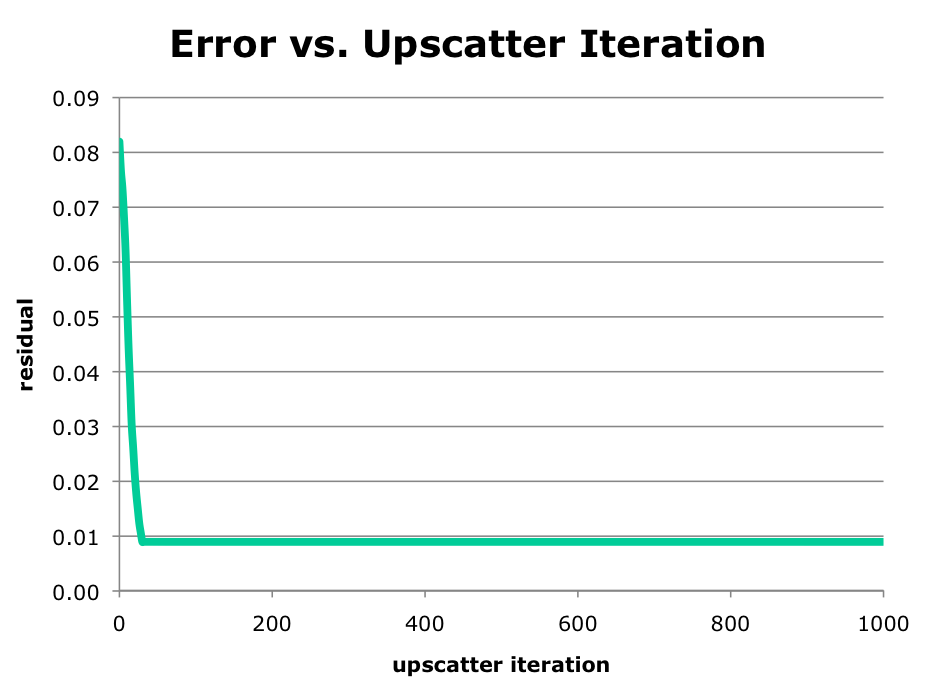
\includegraphics [width=0.75\textwidth, height=0.4\textheight ] {RQIConvergenceFail}
  \end{center}
  \caption{Residual as a Function of Upscatter Iteration Count for One Eigenvalue Iteration in the 2-D MOX Benchmark Problem}
  \label{fig:RQIConvergenceFail}
\end{figure}
%
Figure~\ref{fig:RQIConvergenceFail} shows a plot of the residual vs. multigroup iteration count for one RQI eigenvalue iteration of the 2-D case. It is clear that error reduction stalls and the eigenvector does not converge. Without a good approximation to the eigenvector, the RQ is no longer a valid approximation to the eigenvalue and thus the eigenvalue problem does not converge.

It is likely that the eigenvector does not converge because RQI creates poorly conditioned systems. Krylov methods do not handle ill-conditioned systems very well and may converge extremely slowly. This hypothesis is supported by the fact that during the first eigenvalue iteration the Krylov method does converge fairly quickly. During this first iteration the Rayleigh quotient is computed from the initial guess and is likely not close to the actual eigenvalue. This means the shift on the first iteration is not close to $\lambda_{1}$ so the system will not be too ill-conditioned. After the eigenvector converges on that first iteration it may be that the RQ becomes much closer to $\lambda_{1}$, so the system becomes ill-conditioned and subsequent multigroup iterations do not converge. 

An additional concern is that when the system is ill-conditioned GMRES may no longer be backwards stable. If GMRES is not backward stable, then there is no guarantee that RQI will converge. It is worth noting that there is no evidence that, given a sufficient amount of computing time, RQI would converge to the wrong answer. There is certainly not data to support the claim that RQI will converge to the proper eigenvalue in all cases, but it is heartening to notice there is also not data indicating that it will not. 

Overall, though, the observed behavior strongly suggests that the multigroup Krylov method should be preconditioned so that the eigenvector will converge. If that happens it is likely that RQI will then converge as well. One with preconditioning can the real benefit of RQI be properly investigated.

%-----------------------------------------------------------------------------------------
\subsection{Implications}
Rayleigh quotient iteration is an old method that is an adaptation of shifted inverse iteration. Because the RQ provides an optimal shift, it is expected that using RQI in Denovo will converge in fewer iterations than Power Iteration for some problems, provided that the eigenvector is converged. 

Further, this solver is wrapped around the MG Krylov solver from Chapter \ref{sec:Chp2}. It has already been demonstrated that the energy decomposition works and improves solution time and code scaling for fixed source multigroup problems. It is therefore reasonable to expect that when the method converges, decomposing the entire matrix in energy for eigenvalue calculations will work and provide the same kind of scaling improvement.

The intermediate and large problems that were tested demonstrate that RQI does not converge for even slightly challenging problems. This is probably caused by the poor condition number created by RQI. When the multigroup Krylov solver is not preconditioned it cannot converge the eigenvector in many cases. The incorrect eigenvector subsequently creates an incorrect eigenvalue. 

The small problems showed that RQI can converge in fewer iteration than Power Iteration and may be quite beneficial if the multigroup iterations can be converged. If the MG Krylov solver is preconditioned, then it may be able to converge the eigenvector for cases of interest. To really investigate the benefit of RQI, a good preconditioner is needed. The work in the next chapter is tied to this issue.

RQI has not been applied to the transport equation before because it takes $O(n^{3})$ operations for full dense matrices, and without parallelization in energy it could be prohibitively expensive \cite{Stewart2001}. In the past there was also no motivation to add a shift to make the scattering matrix block dense. If RQI had been used, the system would have been solved with Gauss Seidel and that would have been restrictively slow. The multigroup Krylov algorithm has enabled energy parallelization and made the calculation of the eigenvector tractable. 

Computers that facilitate enough parallelization to decompose in energy and have enough memory to store Krylov subspaces for the full transport equation make combining RQI and MG Krylov possible. The resulting convergence of the eigenvalue should be faster than PI for at least some problems. The energy decomposition will allow eigenvalue calculations to overcome the limitations of KBA and be scaled to many more cores. These ideas have never been used together in this way. New kinds of problems can be solved to a new level of fidelity using these methods. 

    % Chapter 3, ``Eigenvalue acceleration''
 % Prelim, Chapter 4
% by Rachel Slaybaugh

\chapter{Preconditioning}
\label{sec:Chp4}
The new ``grand challenge'' problems facing the nuclear transport community are large and complex. Cutting edge methods are required to solve them. While the second and third chapters discussed methods that enable the solution of such problems, low-cost preconditioners that can reduce the number of iterations needed for convergence will be invaluable. In Benzi et al.'s 2002 survey paper on preconditioning techniques for large linear systems they state ``it is widely recognized that preconditioning is the most critical ingredient in the development of efficient solvers for challenging problems in scientific computation \cite{Benzi2002}.'' 

This is true for Krylov methods in particular because the memory required and cost per iteration increase dramatically with the number of iterations \cite{Benzi2002}. And, as discussed in Chapter \ref{sec:Chp3}, Krylov methods can converge very slowly for poorly conditioned systems. When this happens the eigenvector is not converged in a reasonable number of iterations and RQI cannot converge the eigenvalue. Preconditioning is therefore required to make RQI useful. 

This chapter is about the new preconditioner added to Denovo. First some background information that includes an introduction to preconditioning, an overview of preconditioners used in the nuclear community, and a discussion of multigrid methods is given. Next, past and related work is discussed. Finally the new preconditioner is explained, and results demonstrating its impact are given. 

%-------------------------------------------------------------------------------------------
%-------------------------------------------------------------------------------------------
\section{Background}
The general idea of preconditioning is to transform the system of interest into another equivalent system that has more favorable properties, for example one with a smaller condition number. A preconditioner is a matrix that induces such a transformation by improving the spectral properties of the problem being solved. Let $\ve{G}$ be a non-singular preconditioner, then $\ve{A}x=b$ can be transformed in the following ways \cite{Benzi2002}: 
%
\begin{alignat}{3}
  \ve{G}^{-1}\ve{A}x &= \ve{G}^{-1}b  &  &\text{left preconditioning,} \\
  \ve{AG}^{-1}y &= b, \qquad  &x = \ve{G}^{-1}y \qquad &\text{right preconditioning, and } \\
  \ve{G}_{1}^{-1}\ve{AG}_{2}^{-1}y &= \ve{G}_{1}^{-1}b, \qquad \ve{G} = \ve{G}_{1}\ve{G}_{2}, \qquad  &x = \ve{G}_{2}^{-1}y  \qquad &\text{split preconditioning.} 
\end{alignat}

If $\ve{A}$ and/or $\ve{G}$ are non-normal then each of the preconditioning constructs will likely give different behavior, though they will converge to the same answer because the matrices are similar and therefore have the same eigenvalues  \cite{Benzi2002}. Right preconditioning leaves the right hand side of the equation unaffected and does not change the norm of the residual, which is used for convergence testing in most iterative methods. Right preconditioning is usually preferred over left preconditioning for iterative solvers for this reason \cite{Knoll2004}. A right preconditioner was implemented in this work, and the remaining discussion will be presented in right preconditioner format. 

The matrix $\ve{A}\ve{G}^{-1}$ is not formed in practice. The preconditioner can be applied by using some method to solve $\ve{G}y=c \to y \approx \ve{G}^{-1}c$, or by otherwise implementing the action of $\ve{G}^{-1}$ without ever explicitly forming and inverting $\ve{G}$. There are two extremes between which all other preconditioners lie: $\ve{G} = \ve{A}$, in which case the solution can be found directly, and $\ve{G} = \ve{I}$, which will have no effect \cite{Benzi2002}, \cite{Trefethen1997}. 

Functionally, a good preconditioner should make the system easier to solve and result in faster convergence. It should also be cheap to construct and apply. These tend to be competing goals in that the easier a preconditioner is to construct and apply the less it typically does to improve convergence. A preconditioner is considered good if $\ve{A}\ve{G}^{-1}$ is not too far from normal and its eigenvalues are clustered \cite{Trefethen1997}. 

There are many different types of preconditioners, but they can be put into two general categories: matrix-based and physics-based. Matrix-based preconditioners rely entirely on the structure of the matrix $\ve{A}$ regardless of the physics of the problem. That is, these methods do not change when the underlying problem changes. This can be a very useful property because matrix-based methods are then broadly applicable and do not require any understanding of the physical problem. Extrapolation methods and incomplete factorizations are examples of matrix-based preconditioners \cite{Trefethen1997}.

Physics-based preconditioning uses knowledge about the physics of the problem in question to guide the creation of the preconditioner. This means that some methods only work with certain kinds of problems, and that the preconditioners may have to be tailored or adapted for different applications. However, such methods take advantage of knowing something about the problem and can be more effective than matrix-based methods for the range of problems for which they are intended. Rebalance and synthetic acceleration are examples of physics-based preconditioners \cite{Trefethen1997}.

%-----------------------------------------------------------------------------------------------
\subsection{Preconditioners in the Nuclear Community}
A variety of acceleration methods have been used by the nuclear computational community over the years. This subsection gives a high-level overview of some common methods. In 2002 Adams and Larsen put together a comprehensive overview of the development of iterative methods for solving the \Sn transport equation \cite{Adams2002}. For more detail and history about each method, refer to this publication. 

\subsubsection{Extrapolation Methods}
Extrapolation methods were historically used to accelerate $k$-eigenvalue calculations. These tend to be based on simple iterative solvers or polynomial approximations. One step of a simple iterative method such as Jacobi, Gauss Seidel, or successive over relaxation (SOR) can be used at the outset of a problem to serve as a preconditioner \cite{Trefethen1997}. When applied to neutron transport, an overrelaxation method looks like $\ve{F}_{i+1} = \omega(\tilde{\ve{F}}_i - \ve{F}_i) + \ve{F}_i$ with $1 \le \omega < 2$, where the unaccelerated new iterate for the fission source is designated $\tilde{\ve{F}}_i$ \cite{Lewis1993}.

Polynomial preconditioners create a matrix polynomial $\ve{G}^{-1} = p(\ve{A})$, where $p(\ve{A})$ serves as a polynomial approximation to $\ve{A}^{-1}$. Common polynomial choices are truncated Neumann series and Chebyshev polynomials. An advanced variation of this method is to determine the polynomial coefficients adaptively \cite{Trefethen1997}. When Chebyshev polynomials are applied to the transport equation, $\ve{F}_{i+1} = \ve{F}_i + \alpha_{i+1}(\tilde{\ve{F}}_i - \ve{F}_i) + \beta_i(\ve{F}_i - \ve{F}_{i-1})$, where $\alpha$ and $\beta$ are iteration dependent \cite{Lewis1993}. Neither of these extrapolation methods are widely used today as they have not been very successful in multi-dimensional problems. There are analogous versions of these methods for fixed source problems \cite{Alcouffe1977}.  

\subsubsection{Rebalance}
Rebalance methods are designed to accelerate iteration on the scattering or fission source by imposing a balance condition on the unconverged solution over either coarse or fine regions. If the region is coarse, this is a coarse-grid approximation preconditioner since fine-grid physics are excluded. If the region is fine, this is a local approximation preconditioner where short range effects are permitted and long range interactions are excluded \cite{Trefethen1997}, \cite{Adams2002}.

In either case, the unaccelerated solution is multiplied by a constant in each region that satisfies the balance equation. The rebalance process adjusts the average amplitude of the flux over a region and the iteration adjusts the space-angle distribution. The notion is that these processes work in concert to eliminate all error modes simultaneously \cite{Adams2002}. 

Coarse mesh rebalance (CMR) has been more successful than the fine version and is therefore used more often. In practice, choosing regions properly must be done with care \cite{Lewis1993}. Traditional forms of CMR can be unstable for problems where the spatial mesh is large compared to the neutron mean-free-path and where the scattering ratio is close to unity \cite{Alcouffe1977}. 

\subsubsection{Incomplete Factorizations}
Incomplete factorization methods were first introduced in the 1950s by Buleev, and independently by Varga. In the late 1970s these methods started gaining popularity, and since then have been under active development. The idea is to partially factor the matrix $\ve{A}$ such that the resulting matrices are sparse enough to take advantage of sparse solver methods, but close enough to $\ve{A}$ to be valuable as preconditioners \cite{Benzi2002}.

Incomplete Cholesky (IC) or incomplete LU (ILU) factorization have both been extensively used within the nuclear community. The Cholesky version is used when $\ve{A}$ is symmetric and LU when non-symmetric. Factorizations typically destroy sparsity, resulting in matrices that are denser than the originals and making their use more costly. Different variations of incomplete factorization methods address this by permitting the new matrices to have values only in positions where $\ve{A}$ has values, allowing a prescribed amount of fill in, or only saving entries greater than some tolerance \cite{Trefethen1997}, \cite{Patton2002}, \cite{Oliveira1998}.

\subsubsection{Synthetic Acceleration}
In synthetic acceleration a low-order approximation to the transport operator is used to accelerate the full transport problem \cite{Lewis1993}. If a system is discretized with a high-order method it can be preconditioned with a lower-order approximation. The low-order method is often much sparser than the original, but still captures the general behavior of the problem \cite{Trefethen1997}. This is generally done with either the diffusion equation, giving diffusion synthetic acceleration (DSA), or a transport equation  that is simpler than the one actually being solved, giving transport synthetic acceleration (TSA). These can be used for fission or fixed source problems \cite{Adams2002}. 

%Synthetic methods have at least two iteration stages. The simplest way to illustrate this is to use source iteration for the within-group solver. The first step is a transport sweep, giving:
%%
%\begin{equation}
%  \ve{L}\psi^{(l+\frac{1}{2})} = \ve{S}\psi^{(l)} + q \:, \qquad l \ge 0 \:.
%  \label{eq:synthetic}
%\end{equation}
%%
%Here $l$ is the iteration index, $\ve{L}$ is the transport operator, $\ve{S}$ is the scattering matrix, and $q$ is the external source. Equation \eqref{eq:synthetic} is subtracted from the exact equation to get an expression for an exact additive correction:
%%
%\begin{equation}
%  \bigl( \ve{L} - \ve{S} \bigr)\bigl( \psi - \psi^{(l+\frac{1}{2})} \bigr) = \ve{S}\bigl(\psi^{(l+\frac{1}{2})} - \psi^{(l)} \bigr) \:.
%  \label{eq:correction}
%\end{equation}
%%
%This cannot be solved exactly, but the idea of synthetic methods is to find an $\ve{G}^{-1} \approx (\ve{L} - \ve{S})^{-1}$ that will be easier to evaluate than $(\ve{L} - \ve{S})^{-1}$. Equation \eqref{eq:synthetic} is solved by a high-order scheme and Equation \eqref{eq:correction} is solved with a low-order approximation. If the synthetic system converges, it must satisfy the original transport equation \cite{Adams2002}. 

Original DSA formulations exhibited instability in some instances. In 1977 Alcouffe demonstrated with diamond difference that stability can be obtained by using a consistent spatial differencing scheme \cite{Alcouffe1977}. The transport and diffusion equations cannot be discretized independently or the diffusion equation may not satisfy the original transport equation. The discretization of the diffusion equation must therefore be derived from the discretization of the transport equation such that they are consistent. Alcouffe's idea has since been extended to accelerate currents, to more dimensions, and to different spatial discretizations \cite{Larsen1982}. 

DSA can be implemented a few different ways, each of which performs a transport sweep and then solves a corrected diffusion equation. Different terms in the diffusion equation can be corrected for different problem types \cite{Alcouffe1977}. DSA has been found to degrade in the presence of material discontinuities in addition to when it is not consistently derived. However, Warsa et al.\ found that when DSA is used as a preconditioner for Krylov iterative methods, it is effective even when only partially consistent \cite{Warsa2004}.

To address the concerns about spatial discretization associated with DSA, a low-order transport solve could be used to find the correction term instead. Larsen and Miller developed a method that neglects scattering in the low-order transport equation, but this can cause instability in multi-dimensional problems \cite{Larsen1986}. Ramone et al.\ proposed including some scattering by using a tunable parameter. A high-order transport equation is solved first, then a transport equation with a coarse quadrature and reduced scattering is solved to find the correction that is applied to the new iterate of the scalar flux \cite{Ramone1997}. This algorithm can be viewed as Richardson iteration with a coarse operator preconditioner. Synthetic acceleration methods are widely used and actively researched in the transport community today.

%-----------------------------------------------------------------------------------------------------
\subsection{Multigrid Methods}
The new preconditioner added to Denovo does multigrid in the energy dimension. To understand why multigrid in energy makes sense, why multigrid methods work must be understood. The material presented here is largely from \emph{A Multigrid Tutorial} by Briggs, Henson, and McCormick \cite{Briggs2000}, supplemented by Dr. Strang's lectures on multigrid and preconditioners available as MIT Open Courseware \cite{Strang}.

In what follows, the system of equations will be denoted as $\ve{A}u=b$ where $u$ will represent the exact solution and $v$ will indicate the approximate solution. The algebraic error is given by $e = u - v$. Since $e$ cannot be calculated exactly (otherwise the answer would be known), the residual $r = b - \ve{A}v$ is used instead. A certain grid will be denoted as $\Omega^{h}$ where $h$ is the grid spacing, and vectors on that grid are $u^{h}$. 

The error in any guess can be written as a combination of Fourier modes. A Fourier mode is described by a wavenumber, $k$, which denotes the frequency of oscillation. The $j$th Fourier mode is 
% 
\begin{equation}
    e_{j} = \sin\bigl(\frac{jk\pi}{n}\bigr) \:, \qquad 0 \le j \le n \:, \qquad 1 \le k \le n-1 \:.
\end{equation} 
%
There are $k$ half sine waves that comprise $e$ on the domain of the problem. The term $e_{k}$ indicates an $e$ with wavenumber $k$. The $k$th wave has $\frac{k}{2}$ full sine waves with a wavelength of $\frac{2}{k}$. Modes with wavenumbers in the range $1 \le k \le \frac{n}{2}$ are called low-frequency or smooth modes and those in $\frac{n}{2} \le k \le n-1$ are called high-frequency or oscillatory modes. Figure \ref{fig:FourierModes} shows what a few different modes look like. 
%
\begin{figure}[!ht]
    \begin{center}
      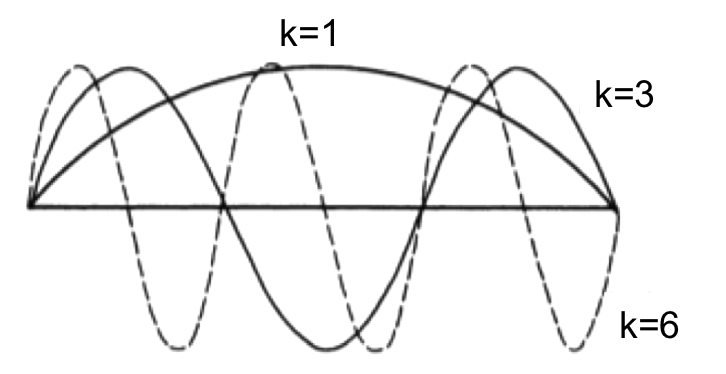
\includegraphics [width=0.45\textwidth, height=0.2\textheight] {FourierModes}
   \end{center}
   \caption{Three Fourier Modes \cite{Briggs2000}}
   \label{fig:FourierModes}
\end{figure}

Iterative methods, also referred to as smoothers or relaxers, remove high frequency error components very quickly, but take a long time to remove the low frequency components. This is illustrated in Figure~\ref{fig:FourierError}, where weighted Jacobi was applied to Fourier modes of different frequencies on an $n$ = 64 grid. The error is reduced much faster for higher modes. 
%
\begin{figure}[!ht]
    \begin{center}
      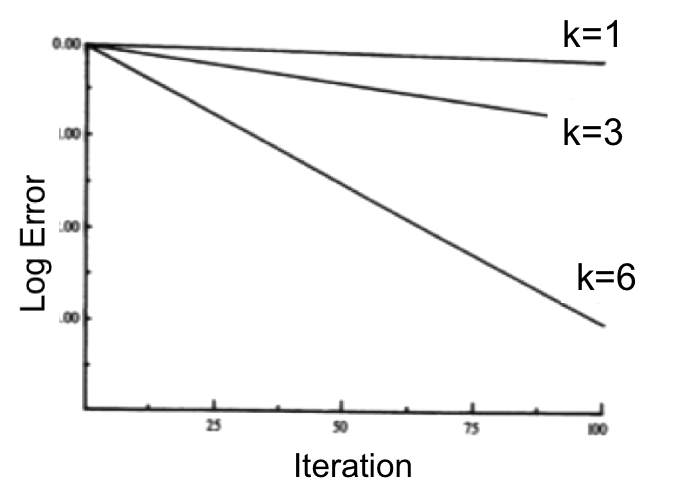
\includegraphics [width=0.5\textwidth, height=0.3\textheight] {FourierError}
   \end{center}
   \caption{Log of Error As a Function of Iteration Count When a Relaxer is Applied to Three Fourier Modes \cite{Briggs2000}}
   \label{fig:FourierError}
\end{figure}
%
The rapid removal of oscillatory and slow removal of smooth error modes is often seen in practice. Figure~\ref{fig:MGerrorExample} shows an error plot that exhibits this behavior
%
\begin{figure}[!ht]
    \begin{center}
      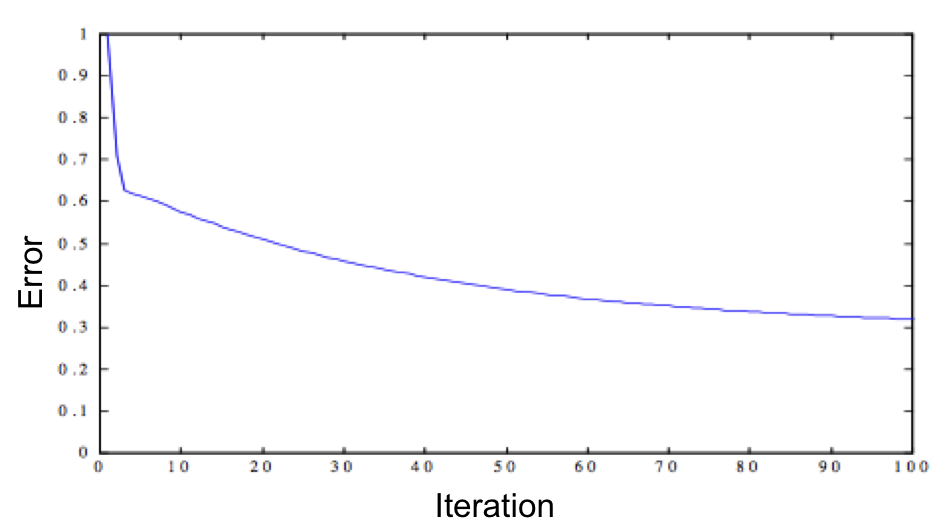
\includegraphics [width=0.7\textwidth, height=0.4\textheight] {MGerrorExample}
   \end{center}
   \caption{Error As a Function of Iteration Count; Oscillatory Components Are Removed Rapidly, Leaving Smooth Components \cite{Briggs2000}}
   \label{fig:MGerrorExample}
\end{figure}

The idea of multigrid methods is to take advantage of the smoothing effect by making smooth error look oscillatory so it can be removed more easily. Error that is low frequency on a fine grid can be mapped onto a coarser grid where it is oscillatory. This change can be thought of as increasing the number of oscillations per grid point. Look at Figure~\ref{fig:FourierGridError} for an example. When $n$ = 12, the maximum number of half-sine waves is 12, so $k$ = 4 is relatively smooth. When mapped to $n$ = 6, $k$ = 4 is relatively oscillatory. 
%
\begin{figure}[!ht]
    \begin{center}
      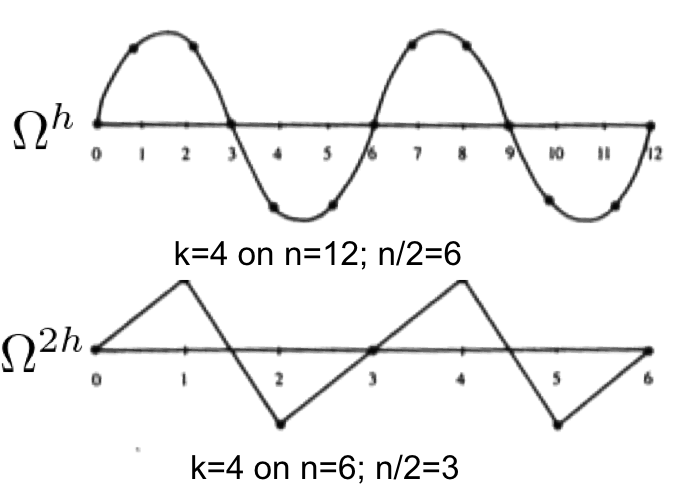
\includegraphics [width=0.55\textwidth, height=0.33\textheight] {FourierGridError}
   \end{center}
   \caption{Relative Oscillation of a Fourier Mode Mapped Between Two Grids \cite{Briggs2000}}
   \label{fig:FourierGridError}
\end{figure}

Using this information, multigrid methods can be understood. The error is mapped from a fine grid to a coarser grid. A smoother is applied on the coarse grid to remove the newly oscillatory error components. The result is mapped back to the fine grid and used to correct the solution there. A few more relaxations are done back on the fine grid. That whole process is called a v-cycle, which is described in Algorithm~\ref{algo:MG}. A call to this method is symbolized as $v^h \leftarrow \ve{G}(v^h, b^h)$ and is effectively doing $v^{h} \approx \ve{G}^{-1}b^{h}$.
%
\begin{algorithm}
  \caption{ Multigrid v-cycle: $v^h \leftarrow \ve{G}(v^h, b^h)$}
  \label{algo:MG}
  \begin{list}{}{\hspace{2.5em}}
    \item Relax $\nu_1$ times on $\ve{A}^h u^h = b^h$ on the fine grid $\Omega^h$ using initial guess $v^h$.
    \item Compute the residual $r^h = b^h - \ve{A} v^h$. 
    \item Using some restriction operator, $\ve{R}_h^{2h}$, restrict the residual to a coarser grid: $r^{2h} =  \ve{R}_h^{2h} r^h$. 
    \item Solve the residual equation $\ve{A}^{2h} e^{2h} = r^{2h}$ on the coarse grid $\Omega^{2h}$. 
    \item Using some prolongation operator, $\ve{P}_{2h}^h$, prolong (interpolate) the coarse grid error back to a finer grid: $e^h = \ve{P}_{2h}^h e^{2h}$. 
    \item Add the error to the fine grid guess: $v^h \leftarrow v^h + e^h$. 
    \item Relax $\nu_2$ times on $\ve{A}^h u^h = b^h$ on $\Omega^h$ to get an improved solution. 
   \end{list}
\end{algorithm}

The details of how restriction and prolongation are done are problem dependent. Simple iterative schemes can have very simple operators while more complex schemes may require more complex mappings. Other implementation choices are what relaxer to use and how many relaxations to do on each grid.

There are many variations of how multigrid methods are put together. All methods, however, are built on the basic v-cycle correction scheme. A V-cycle is an extension of the v-cycle. Instead of only using two grids, many grids are used. The problem is restricted from grid to grid until it is on some grid which is coarse enough to directly invert the equations. Then the errors are prolonged back up the chain, continuously correcting on finer grids, until the finest grid is reached. Multigrid methods are differentiated by how many times the V-cycle is done and how many grids are used. A five-grid V-cycle can be seen in Figure~\ref{fig:Vcycle} (a). A W-cycle is when V-cycles are repeated to further improve the answer. An example can be seen in Figure~\ref{fig:Vcycle} (b). 
\begin{figure}
    \begin{center}
      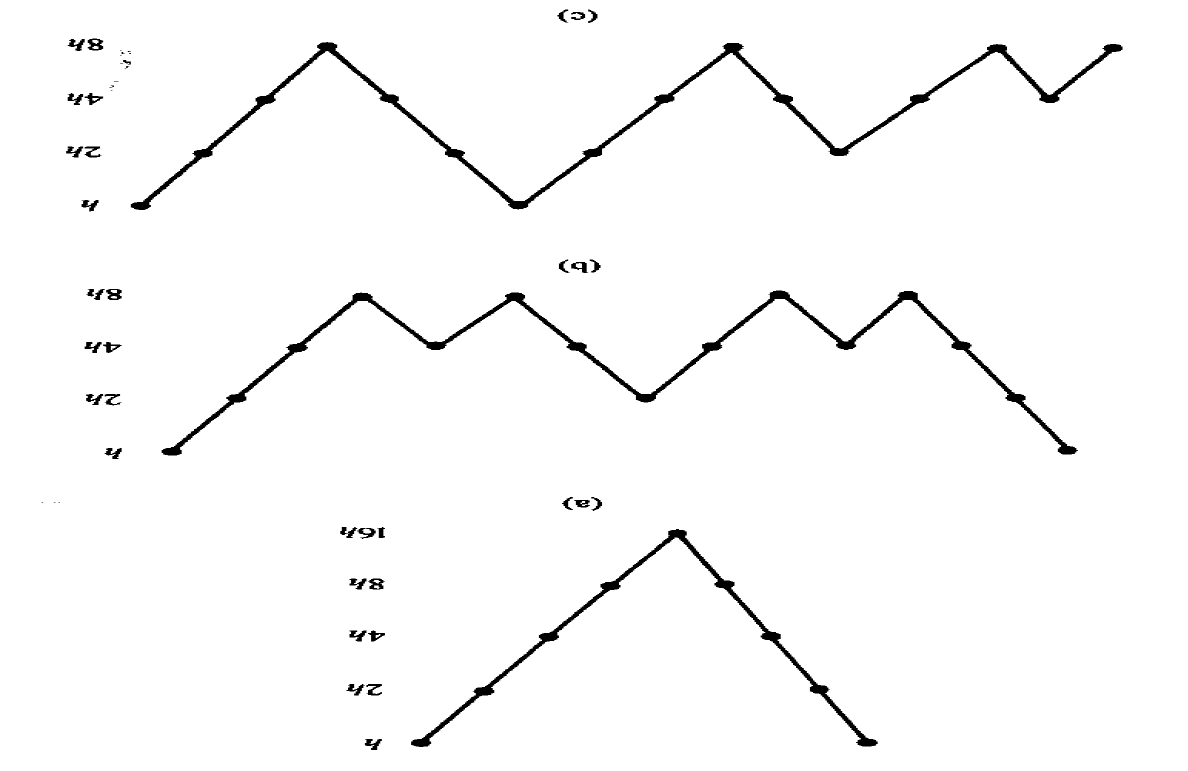
\includegraphics [width=0.7\textwidth, height=0.7\textheight, angle=180 ] {multigridFig}
   \end{center}
   \caption{Grid Schedule for (a) a V-cycle, (b) a W-cycle, and (c) a Full Multigrid Pattern \cite{Briggs2000}}
   \label{fig:Vcycle}
\end{figure}

Multigrid can also be used to obtain an initial guess where much of the smooth error has been removed. This is called nested iteration, and the iterations begin on the coarsest grid and move up to the finest grid. If nested iteration is combined with V-cycles, the full multigrid method (FMG) is obtained, as seen in Figure~\ref{fig:Vcycle} (c). A call to any of the combinations of v-cycles is denoted $v \leftarrow \ve{G}(v, b)$. The optimal combination of grids and cycles may depend on problem type. The addition of more grids and cycles will reduce error, but at an added cost. 

Multigrid methods can be thought of as stationary iterative schemes that can be used alone or as accelerators for other methods. In the past these methods were highly problem specific and only applied to second-order elliptic PDEs. Over time they have been extended to different problem types, geometries, and discretizations \cite{Benzi2002}. 

%-------------------------------------------------------------------------------------------------------
%-------------------------------------------------------------------------------------------------------
\section{Past Work}
This section discusses some past work from most of the categories of preconditioners that were presented above. The focus is on methods that have been used to precondition Krylov solvers and on multigrid methods. This section is intended to illustrate the need for preconditioning Krylov methods in transport and to demonstrate the new preconditioner's originality. 

As an aside, it is important to note that how well a preconditioner is going to perform for a certain problem when using Krylov methods cannot be known \emph{a priori}. At this time there are no set methods or procedures for predicting preconditioner behavior with Krylov methods. As a result, preconditioning Krylov methods is somewhat ``guess and check.'' Despite this, the rewards of preconditioning Krylov methods ensure that they are an essential part of their practical use \cite{Knoll2004}, \cite{Benzi2002}. 

%-------------------------------------------------------------------------------------------------------
\subsection{Rebalance}
CMR has been widely used in transport codes since at least the 1970s and new variants of it are being applied to Krylov solvers \cite{Dahmani2002}, \cite{Yamamoto2005}. For example, Dahmani et al.\ investigated using GMRES and preconditioned GMRES for solving the 3-D transport equation using the method of characteristics (MOC) in 2005. Self-collision rebalance (SCR) was used as a left preconditioner. SCR uses the probability of a region scattering particles to itself to rebalance the energy distribution in each region. MOC is quite different from \Sn and requires a specific derivation to be able to use GMRES \cite{Dahmani2002}. 

%-------------------------------------------------------------------------------------------------------
\subsection{Incomplete Factorizations}
Incomplete factorizations have also been used to precondition Krylov methods, though without much success for large transport problems. Patton and Holloway investigated the use of a variety of preconditioners for GMRES to solve the multi-group, diamond-difference, 1-D, \Sn equations. They compared matrix-based and physics-based right preconditioners. A variety of factorization methods, the matix-based preconditioners, were considered: ILU(0), modified ILU(0) (MILU), ILU($\tau=10^{-4}$), ILU($p=10$), and ILU($\tau=10^{-4}, p=10$), where $\tau$ is the drop tolerance and $p$ indicates the amount of fill-in allowed. A single integer indicates the fill-in limit. 

The bandwidth of $\ve{A}$ increases as the number of energy groups and/or discrete ordinates increases \cite{Patton2002}. Here, the bandwidth of the matrix is $2GM$ where $G$ is the number of energy groups and $M$ is the number of discrete ordinates. The computational time required by ILU factorization increases with the bandwidth of $\ve{A}$. This makes factorization methods unattractive as accelerators for finely discretized problems. This prompted Patton and Holloway to consider physics-based methods. 

%A matrix splitting was chosen such that the original problem formulation was written as:
%%
%\begin{equation}
%  \ve{L}\psi - \ve{S}_{in}\psi = \ve{Q} \:,
%\end{equation}
%%
%where $\ve{L}$ is the streaming plus removal term, $\ve{S}_{in}$ is the inscattering source, and $\ve{Q}$ contains the external source. Patton and Holloway use $(\ve{L} - \ve{S}_{down})^{-1}$ as the preconditioner, where  $\ve{S}_{down}$ is the downscatter part of the $\ve{S}$ matrix. They use source iteration as the within-group solver such that each new guess is obtained by applying $(\ve{L} - \ve{S}_{down})^{-1}(\ve{S}_{in} - \ve{S}_{down})$ to the old guess. 
A matrix splitting method was chosen that used physics rather than generic structural properties to inform how to do the splitting. They used source iteration as the within-group solver. For the 1-D case they found that this physics-based preconditioner was faster than the matrix-based factorization preconditioner, but that DSA was faster than both \cite{Patton2002}. This is not surprising because DSA is so effective for 1-D with diamond difference. 

In 2004 Chen and Sheu compared preconditioned conjugate gradient methods with SOR for 3-D, multigroup neutron transport. They used ILU and MILU to precondition both conjugate gradient squared (CGS) and BiCGSTAB. They chose these iterative techniques because they have good residual error control procedures that give good convergence rates in general \cite{Chen2004}.

Kozlowski, Downar, and Lewis investigated a Krylov preconditioning method for the multi-group $SP_3$ transport equations. This method involves reordering the fluxes to facilitate the use of block ILU as the preconditioner. This idea worked well for small problems, but may require too much storage for large problems \cite{Kozlowski2003}.

%-------------------------------------------------------------------------------------------------------
\subsection{Synthetic Acceleration}
DSA has been under continuous development since Alcouffe's 1977 paper. For example, a recent research string began when Wareing, Larsen, and Adams developed a simple DSA scheme for bilinear discontinuous (BLD) discretizations in 2-D. An unconditionally efficient multigrid technique for solving these 2-D, BLD equations was derived by Morel, Dendy, and Wareing. This was later extended to bilinear nodal differencing and bilinear characteristic differencing \cite{Adams2002}. New versions of DSA are applied to Krylov solvers in current transport codes.

Very recently Rosa et al.\ performed detailed Fourier Analysis on TSA combined with Inexact Parallel Block-Jacobi (IPBJ) splitting applied to the one- and two-dimensional transport cases. They noted that both experience in the nuclear community and analytical work have shown that solution methods such as GMRES(m) can stagnate for problems containing optically thin spatial regions. Rosa et al.'s analysis and results show that using modified TSA improves the spectral properties such that convergence can be obtained using a relatively small m when using GMRES(m) \cite{Rosa2010}.

\subsubsection{DSA in Denovo}
Denovo has the option to use DSA to precondition the within-group transport equation, $\bigl(\ve{I} - \ve{DL}^{-1}\ve{MS}_{gg}\bigr) \phi_{g} = \ve{DL}^{-1}Q_{g}$, which works very well when using a Krylov method. High-frequency error modes are what often cause instability in DSA. Krylov iteration, like iterative methods in general, will rapidly damp such oscillatory modes. Eliminating the high-frequency error enables the removal of the consistency requirement since DSA is not likely to fail when those error modes are gone \cite{Evans2009d}. This means DSA can be applied successfully for a variety of spatial discretizations. 

The DSA-preconditioned one-group equation is:
%
\begin{equation}
  \bigl(\ve{I} + \ve{PC}^{-1}\ve{RS}\bigr) \bigl(\ve{I} - \ve{DL}^{-1}\ve{MS}\bigr) \phi = \bigl(\ve{I} + \ve{PC}^{-1}\ve{RS}\bigr)\ve{DL}^{-1}\bar{Q} \:. 
  \label{DSA1group}
\end{equation}
%
Here $\ve{C}$ is the diffusion operator defined in Appendix~\ref{sec:AppendixA}; $\ve{R}$ is the restriction operator that maps the transport solution onto the diffusion vector; and $\ve{P}$ is the projection operator that maps the diffusion vector onto the transport solution. Denovo does not actually form these operators, instead it solves the diffusion equation and updates the $\phi_{00}$ moments. In practice this means that for a Krylov iteration
%
\begin{equation}
  \ve{C}z = \ve{RS}\bigl(\ve{I} - \ve{DL}^{-1}\ve{SM}\bigr) v
\end{equation}
%
is solved for each group. In Denovo, DSA has been found to be beneficial for diffusive problems with high scattering ratios that are close to being isotropic \cite{Evans2009d}. This is consistent with experiences of the wider nuclear community.

%-------------------------------------------------------------------------------------------------------
\subsection{Multigrid Methods}
Beginning in the late 1980s, the nuclear community started using spatial \mg and/or angular \mg as both solvers and preconditioners. The first use of spatial \mg for transport equations in 1-D and 2-D was investigated by Nowak et al. Since that time \mg has been used in multiple dimensions, for both isotropic and anisotropic scattering, and for various spatial discretizations \cite{Adams2002}. Some highlights from recent work are discussed below. All are applied to the \Sn neutron transport equation unless otherwise noted. 

In 1996 Sjoden and Haghighat used a simplified spatial \mg method that does not use the residual as a solver for the 3-D, parallel code PENTRAN \cite{Sjoden1996}. In 1998 multigrid in space and multigrid in angle were used as preconditioners for Krylov methods and were tested for the 1-D, one-group, modified linear discontinuous (MLD) neutron transport equations by Oliveira and Deng. They looked at isotropic scattering without absorption, isotropic with absorption, and anisotropic cases. They had better results with multigrid than when using ILU as a preconditioner \cite{Oliveira1998}.

In 2007 Chang et al.\ used 2-D spatial \mg for the isotropic scattering case with corner balance finite difference in space and a four-color block-Jacobi relaxation scheme. A bilinear interpolation operator and its transpose were used for grid transfer. The method had some trouble with heterogeneous problems. The authors assert their algorithm is parallelizable \cite{Chang2007}.

In 2010 Lee developed a method to do \mg in space and angle simultaneously for two and three dimensions, isotropic and anisotropic scattering, one energy group, and a variety of spatial discretizations. The method can perform \mg in only space, only angle, or some combination there of. It also handles thick and thin cells \cite{Lee2010}.

This list is hardly comprehensive, but is intended to be representative of new and recent developments in this area. No cases were found where \mg was used in the energy variable either as a solution technique or as a preconditioner. 

\subsubsection{Two-Grid Acceleration}
The two-grid acceleration method developed by Adams and Morel was one of the earlier spatial \mg methods and it has been built upon by others \cite{Adams1993}. It is intended to accelerate convergence of the outer iterations for the transport equation when upscattering is present; the outer iteration method is Gauss Seidel and the method is only applied to upscattering groups. The original work was done for slab geometries with linear discontinuous (LD) discretization. The general approach is expounded upon here to provide an example of \mg methods applied to the transport equation and because a variation of this method is used in Denovo. 

Adams and Morel create a within group error equation by subtracting the GS equation from the transport equation. If the error in iteration $k$ is $\epsilon^k$ and the $l$th moment of the residual is $R_l^k$, then for group $g$ in 1-D this gives:
%
\begin{align}
   \mu \frac{\partial \epsilon_{g}^{k+1}(\mu)}{\partial x} + \Macro_{t,g} \epsilon_{g}^{k+1}(\mu) &= \sum_{l=0}^{L}\frac{2l+1}{4\pi} \bigl( \sum_{g'=1}^{G}\Macro_{s,g' \to g, l} \epsilon_{g',l}^{k+1} 
   +  R_{g,l}^{k+1}\bigr) P_{l}(\mu) \:,\label{eq:GSerror} \\
  \epsilon_{g}^{k+1}(\mu) &= \psi_{g}(\mu) - \psi_{g}^{k+1}(\mu) \:, \\
  \epsilon_{g',l}^{k+1} &= 2\pi \int_{-1}^{1}\epsilon_{g'}^{k+1}(\mu') P_{l}(\mu') d\mu' \:, \\ 
  R_{g,l}^{k+1} &=  \sum_{g'=g+1}^{G}\Macro_{s,g' \to g, l} \bigl( \phi_{g',l}^{k+1} - \phi_{g',l}^{k} \bigr) \:.
\end{align}
%
The diffusion approximation is applied to Equation \eqref{eq:GSerror}, giving a coarse grid equation. The fine grid is the \Sn equations for the upscattering groups. The coarse grid is the isotropic, one-group, diffusion equation. 

It is assumed that the zeroth moment of the error is a product of a spectral shape function, $\xi_g$ and a space-dependent modulation function, $E(x)$, giving
%
\begin{align}
  \epsilon_{g,0}^{k+1}(x) &= E(x)\xi_{g} \:, \text{ and} \label{eq:errorExpand} \\
  \sum_{g=1}^{G} \xi_{g} &= 1 \:.
\end{align} 
%
The spectral shape function corresponds to the slowest converging error mode, i.e.\ the mode to be eliminated. To find the shape function, Fourier analysis is performed on the GS iterative method. The zeroth moment of the cross sections is used to form the Fourier matrix, and then an eigenproblem can be formed. The spectral radius of the isotropic GS matrix is the eigenvalue, and the corresponding eigenvector is the shape function. Because the shape function is dependent on materials, one such calculation must be done for each material region. Note that by using the zeroth moment only the isotropic component of the solution is accelerated.

To restrict the residual, which is used as the source, to the coarse grid in the angular dimension, the anisotropic terms are truncated. To restrict to one energy group, the residual is simply summed in energy. The coarse grid equation is then solved on the coarse grid for the error. That error is prolonged to the fine grid and used to correct the flux there. The anisotropic terms are not recovered in the prolongation. The shape functions are used to expand the one group diffusion solution (error) into multiple groups. 

The coarse grid diffusion equations that result from Equations \eqref{eq:GSerror} and \eqref{eq:errorExpand} differ slightly in form from the standard diffusion equation in that there is an extra term containing the gradient of the shape function. This is zero in homogeneous regions, but undefined at material interfaces. Adams and Morel found that neglecting the gradient term all together still gave good results for their test problems. This may not be true for more complex cases.

The two-grid method requires the diffusion operator to be consistent with the transport operator, just like in DSA. This requirement can be difficult to meet for multi-dimensional problems, particularly for some spatial discretizations \cite{Adams1993}. 

\subsubsection{Two-Grid in Denovo}
\label{sec:TTG}
Denovo has a two-grid acceleration scheme based on the one developed by Adams and Morel. As noted above, the iteration procedure uses a collapsed one-group diffusion equation to correct the low-order Fourier modes \cite{Adams1993}. Because of the consistency requirement for the discretization of the diffusion operator in multi-dimensional and multi-material problems, this method can fail for systems of interest \cite{Evans2009d}. 

The original two-grid method was modified by Evans et al.\ to make it applicable for the desired cases by using a one-group transport equation instead of the diffusion equation. The modified method is called transport two-grid (TTG). Adams and Morel showed that the slowest converging spatial modes are diffusive and can be exactly computed in the infinite homogeneous case. To preserve this, the TTG method gives the correct error estimation in that limit \cite{Evans2009d}. 

The cross sections used in TTG are therefore calculated to give the same energy-collapsed cross sections as the diffusion equation for the infinite homogeneous case, as seen in Equations \eqref{TTGxsecs1} and \eqref{TTGxsecs2}. TTG solves a one-group transport equation for the low-order error in each GS iteration, where $[g1, g2]$ is the group range of the upscatter block:
%
\begin{align}
  \ve{\hat{\Omega}} \cdot \nabla \psi_{\epsilon} &+ \bar{\Macro}\psi_{\epsilon} = \frac{1}{4\pi}\bar{\Macro}_{s}\phi_{\epsilon} + \frac{1}{4\pi}\bar{R} \:, \\
  \bar{\Macro} &= \frac{1}{\sum_{g=g_1}^{g_2} \frac{1}{\Macro^g}\zeta^g} \label{TTGxsecs1} \:,\\
  \bar{\Macro}_{s} &= \frac{1}{\sum_{g=g_1}^{g_2} \frac{1}{\Macro^g}\zeta^g} - \sum_{g=g_1}^{g_2} \bigl(\Macro^g\zeta^g - \sum_{g'=g_1}^{g_2} \Macro_{s0}^{gg'} \zeta^{g'} \bigr) \label{TTGxsecs2} \:. 
\end{align}
%
The spatial components of the error are $\psi_{\epsilon}$ and $\phi_{\epsilon}$; $\bar{R}$ is the residual. Just as in the original method, it is assumed that the error is separable in space and energy at each iteration: $\epsilon_g^k = \phi_g - \phi_g^k = \phi_{\epsilon}(\vec{r})\zeta^g$, where $\zeta^g$ is a material-dependent spectral function \cite{Evans2009d}. 

To execute the TTG scheme in Denovo, a transport sweep in conducted in each group, a residual is calculated, the low-order transport solve described above is performed, an error form of the transport sweep is conducted, and the scalar flux is updated. All of that can be seen in the following equations: 
\begin{align}
  \ve{L}_g \psi_g^{k+\frac{1}{2}} &= \ve{M}\bigl(\ve{S}_{gg}\phi_g^{k+\frac{1}{2}} + \sum_{g'=g_1}^{g-1} \ve{S}_{gg'}\phi_{g'}^{k+\frac{1}{2}} + \sum_{g'=g+1}^{g_2}\ve{S}_{gg'}\phi_{g'}^k \bigr) + q_{e,g}  \:, \\
  R^{k+\frac{1}{2}}_g &= \ve{M} \sum_{g'=g+1}^{g_2}\ve{S}_{gg'} \bigl( \phi_{g'}^{k+\frac{1}{2}} - \phi_{g'}^k \bigr) \:, \qquad l = m = 0 \:, \\
  \bar{\ve{L}}\psi_{\epsilon} &= \ve{M\bar{S}} \phi_{\epsilon} + \bar{R} \:, \qquad l = m = 0 \:, \label{TTGerrorEqn} \\
  \phi_g^{k+1} &= \phi_{g}^{k+\frac{1}{2}} + \phi_{\epsilon}\zeta^g \:, \qquad l = m = 0 \:.
\end{align}
The operators with over-bars use the collapsed cross sections given in Equations \eqref{TTGxsecs1} and \eqref{TTGxsecs2}, and $\bar{R} = \sum_{g=g_1}^{g_2} R_g^{k+\frac{1}{2}}$. 

The $\zeta_g$ term is calculated from the eigenvalue problem obtained through Fourier analysis of the GS method using isotropic scattering, just like the original two-grid method:
%
\begin{equation}
  \bigl(\ve{T} - \ve{S}_L + \ve{S}_D\bigr)^{-1} \ve{S}_U\zeta = \rho\zeta \:,
\end{equation}
where $\ve{T}$ is the diagonal, total cross section matrix. As with the original two-grid method, the TTG method is limited to correcting only the isotropic flux moments. This is an adequate limitation as these moments are dominant in thermal groups where upscattering is most prevalent\cite{Evans2009d}.   

The additional cost of the method is like solving one extra group, so for cases with many upscattering groups the cost can be amortized. The acceleration equation can be preconditioned with DSA for additional speed. Finally, a reduced quadrature set can be used when solving Equation~\eqref{TTGerrorEqn} to limit the cost. Some test problems have shown TTG to be quite effective in improving the speed of convergence for upscatter problems when compared to unaccelerated GS \cite{Evans2009d}.

%-------------------------------------------------------------------------------------------------------
Clearly, a wide variety of preconditioning techniques have been applied to the neutron transport equation. It is worth noting that many of these methods are dependent upon the choice of spatial discretization employed, only apply to within group iterations, or have other important limitations. Preconditioning Krylov methods for solving the neutron transport problem is an active and vital area of research where much progress has been made and in which there is still much room for development. 

%-------------------------------------------------------------------------------------------------------
%-------------------------------------------------------------------------------------------------------
\section{Multigrid in Energy}
Preconditioning is a very important part of increasing the robustness of Krylov methods. This is particularly true in this work for two reasons. The first is that the multigroup Krylov solver can create very large Krylov subspaces because it forms the subspaces with multiple-group-sized vectors. As a result, any reduction in iteration count will have a large benefit in terms of both memory and cost per iteration. The second is that preconditioning is needed to compensate for the ill-conditioned systems created by RQI so that the eigenvector can be converged. 

A new physics-based, multigrid-in-energy preconditioner has been added to Denovo to improve the performance of the Krylov solves. Choosing a physics-based preconditioner supports the goal of accelerating a code that solves a specific equation rather than developing an all purpose preconditioner. It makes sense to take advantage of information specific to the neutron transport equations. Previous work has shown that physics-based preconditioners often provide more benefit than matrix-based methods. Further, the matrix $\ve{A}$ is never formed in Denovo, ruling out matrix-based preconditioners. 

Among physics-based preconditioners, a multigrid method was selected because they have been generally successful at accelerating the transport equation, and the residual behavior in the Krylov iterations inside RQI looks like the ideal case for multigrid methods.

The preconditioner was designed to take advantage of the energy decomposition added by the MG Krylov method. Having grids in energy rather than space or angle means that each energy set can use its own grids without communicating with other sets. An additional benefit is the simplicity of energy grids. Energy is one dimensional, which makes the grids much less complex (and likely less costly) than angular or multi-D spatial grids. 

To make energy grids, the energy group structure is coarsened so each lower grid has fewer groups on it. The finest grid is the input energy structure, and the coarsest grid has one or a few groups. Each level has half as many groups as the previous level, rounded up if applicable. This is conceptually straightforward because the energy groups can be combined (restricted) and separated (prolonged) linearly. 

There are a variety of options that must be considered in designing a multigrid scheme: the restriction and prolongation operators, the relaxation method, the number and/or pattern of V-cycles to use, the number of relaxations to do on each grid level, and the depth of the V-cycle. Among these the number of number of V-cycles and the number of relaxations per level have been implemented as user input options; the others are fixed. 

The implemented restriction operator is a simple averaging scheme. Neighboring fine data are averaged together to make coarse data. Recall that in multigrid methods the variables being restricted and prolonged are error modes. For a grid with spacing $h$ and a next-coarser grid $2h$, the errors are restricted as $e_{g}^{2h} = \frac{1}{2}(e_{2g}^{h} + e_{2g+1}^{h})$ for $g = 1,...,G$, where $G$ is the number of groups on the coarse grid and $2G+1$ is the number of groups on the fine grid. If there are an odd number of groups the lowest energy group's datum is just copied. This scheme was chosen so that the thermal energy groups would retain more granularity, which should improve accuracy for thermal reactors. The errors are restricted every time there is a transfer to a coarser grid.

The cross sections are restricted from the finest to the coarsest grid during problem initialization and they do not change thereafter. The total and fission cross sections are restricted in the same way as the errors. Scattering is slightly more complicated since it has two indices, $g$ and $g'$. When there are an even number of groups all cross sections are treated the same way. For $g' = 1,..., G'$ and $g = 1, ..., G$,
\begin{equation}
  \Sigma_s^{2h}(g,g') = \frac{1}{4}[\Sigma_s^{h}(2g,2g') + \Sigma_s^{h}(2g+1,2g') + \Sigma_s^{h}(2g,2g'+1) + \Sigma_s^{h}(2g+1,2g'+1)] \:. 
  \label{eq:XSSeven}
\end{equation}
% 
Unless there is upscattering in every group, some of the entries in Equation~\eqref{eq:XSSeven} will be zero. When there are an odd number of groups Equation \eqref{eq:XSSeven} is used until $g=G-1$ and $g'=G'-1$. For the last group
  \begin{align}
    \Sigma^{2h}_s(G,g') &= \frac{1}{2}[\Sigma^{h}_s(2G,2g') + \Sigma^{h}_s(2G,2g'+1)] \qquad \text{for } g' = 0,...,G'-1 \:,\nonumber \\
    \Sigma^{2h}_s(g,G') &=  \frac{1}{2}[\Sigma^{h}_s(2g,2G') + \Sigma^{h}_s(2g+1,2G')] \qquad \text{for } g  = 0,...,G-1 \:,\nonumber \\
    \Sigma^{2h}_s(G,G') &= \Sigma^{h}_s(2G,2G') \nonumber \:.
  \end{align}

The cross sections could be flux-weighted and re-restricted every time a new value for the flux were available, i.e.\ every new application of the preconditioner, to more accurately preserve physics. The experience of the computational community has been that preconditioners do not have to rigorously and accurately preserve physics to be effective and the tradeoff between the physics preservation and the performance of the preconditioner cannot be known \emph{a priori}. The assumption in this work is that the cost of recomputing the cross sections in every preconditioner application is greater than the benefit of more accurately representing the physics.

To prolong from a coarse to a fine grid, the points that line up between the grids are mapped directly: $e_{2g}^{h} = e_{g}^{2h}$. To fill in the intermediate points on the fine grid, the adjacent coarse values are averaged: $e_{2g+1}^{h} = \frac{1}{2}(e_{g}^{2h} + e_{g+1}^{2h})$. The errors are prolonged every time there is a transfer to a finer grid. Since cross sections do not change they are never prolonged. 

There are other restriction and prolongation operators that are more rigorous and would preserve more accuracy when transferring between grids than the implemented ones. For example, a full weighting restriction operator would be more rigorous in combination with the current prolongation method than the current restriction operator is \cite{Briggs2000}. This change would be straightforward to implement. 

An example of a more complex prolongation operator that would be more accurate would be to use shape functions to prolong from a coarse grid to a fine grid. The shape functions could be based on the previous iterate of the fine-grid vector, some known desirable expansion, etc. Such a change would be more difficult to implement and require more research. 

These issues were not investigated in this work since the chosen operators, which were simple to code and check for correct implementation, were sufficient in practice. Any errors that may have been added by the restriction and prolongation operators were largely removed by the relaxations. In addition, because this is a preconditioner all of the pieces do not need to be rigorous. It is likely not valuable to spend time on complex grid transfer operators. However, it could be of value to investigate other simple operators. 

The user chooses the number of V-cycles done on each preconditioner application, $v \leftarrow \ve{G}(v,b)$. Recall that one V-cycle, seen in Figure~\ref{fig:Vcycle} (a), goes from the finest grid to the coarsest grid and back up to the finest. The input option specifies the number of the large Vs that are concatenated together. The default number of V-cycles is 2. Each additional V-cycle should remove more error, but also has a computational cost. 

At this time the depth of the V-cycle is determined by the number of groups such that the grids will be coarsened until there is only one energy group. The number of grids needed is given by \cite{BinaryTree2011}
\begin{equation}
  \text{floor}\bigl( \log_{2}(G-1) \bigr) + 2 \:.
  \label{eq:NumGrids}
\end{equation}
%
How this is handled when using energy sets is discussed below. The depth of the cycle is an option that could be changed in the future if it is found that restricting down to only one group is unnecessary, particularly if there are a large number of groups. Investigating the optimal V-cycle depth is an important issue, but beyond the scope of this work. 

Some number of relaxations are performed on each level while traversing down and up the grids in a V-cycle. The number of relaxations per level, $\nu_{1,2}$ from Algorithm~\ref{algo:MG}, is a user input choice with a default of 2. Doing more relaxations per grid should remove more error, but also has a computational cost. The implemented relaxation method is weighted Richardson iteration, whose $k$th step is
%
\begin{equation}
  \phi^{k} = \phi^{k-1} + \omega^{k}\ve{P}^{-1}(b^{k-1} - \ve{A}\phi^{k-1}) \:.
  \label{eq:Richardson}
\end{equation}
%
$\ve{P}$ is some easily invertible matrix, the details of which determine exactly what method is being used. If $\omega^{k}$ is constant then this is the stationary Richardson method \cite{Moore1999}. 

In this work $\ve{P} = \ve{I}$, $\ve{P}^{-1} = \ve{I}$, and $\omega$ is a constant selected by the user that defaults to 1. When applied to the Transport equation, this looks like
%
\begin{align}
  \phi^{k} &= \phi^{k-1} + \omega\bigr(b^{k-1} - (\ve{I} - \ve{TMS})\phi^{k-1}\bigl) \:, \text{ or} \nonumber \\
  \phi^{k} &= \bigr(\ve{I} + \omega(\ve{TMS} - \ve{I})\bigl)\phi^{k-1} + \omega b^{k-1} \:.
  \label{eq:relax}
 \end{align}
  
An important principle is that the preconditioner is only attempting to roughly invert $\ve{A}$, so choosing to simplify the preconditioner beyond the solution method alone, i.e.\ using Richardson instead of Krylov, is reasonable. In this vein it is possible to use a smaller angle set in the preconditioner than the rest of the code. For example, the whole problem can be solved at $S_{10}$, but the preconditioner would only use $S_{2}$. There is an input option to specify what to use in preconditioner; the default is to use the same angle set as the rest of the problem. At this time this option has only been implemented for vacuum boundary conditions. 

Recall that right preconditioning is applied as $\ve{A} \ve{G}^{-1} \ve{G} \phi = b$, where $\ve{A} = \ve{I} - \ve{TMS}$. To implement this in Denovo, $y$ was defined as $\ve{G}\phi$ and the problem was broken into two steps: 
%
\begin{align}
  \text{with a Krylov method solve} \qquad \ve{AG}^{-1}y &= b \:. \label{eq:PrecondKrylov} \\
  \text{After finding }y\text{, the final step is} \qquad \phi &= \ve{G}^{-1}y \:. \label{eq:PrecondPhi}
\end{align}
%
The Krylov solvers cannot be modified easily because they are provided by an external library, so the preconditioner must be applied to the iteration vector that is handed to the solver to carry out Equation~\eqref{eq:PrecondKrylov}. Equations~\eqref{eq:invertG} and \eqref{eq:ApplyA} show how this is accomplished for each application of the Krylov solver. Equation~\eqref{eq:findPhi} shows how Equation~\ref{eq:PrecondPhi} is solved.  

Let $v^{j}$ be an iteration vector that represents $y$, and let $z^{j}$ be an intermediate iteration vector. In each step below the equations are written three ways to show what is going on algorithmically: the equation being solved, the symbolic representation of the outcome, and the way this is written in multigrid syntax. The first thing is to apply the preconditioner to the intermediate vector to affect the inversion of $\ve{G}$. For Krylov iteration index $j = 1, ..., J$:
%
\begin{align}
  \ve{G}z^{j} &= v^{j} \:,  \label{eq:invertG} \\
  z^{j} &\approx \ve{G}^{-1}v^{j} \:, \nonumber \\
  z^{j} &\leftarrow \ve{G}(z^{j}, v^{j}) \:. \nonumber
\end{align}
%
Next, apply the operator $\ve{A}$ to $z^{j}$ and set it equal to $v^{j+1}$:
\begin{align}
  v^{j+1} &= \ve{A}z^{j} \:,   \label{eq:ApplyA} \\
  v^{j+1} &\approx \ve{AG}^{-1}v^{j} \:, \nonumber \\
  v^{j+1} &= \ve{A}[z^{j} \leftarrow \ve{G}(z^{j}, v^{j})] \:. \nonumber
\end{align}
%
Once $v$ has converged, $y = v^{J}$. The final step is to apply the preconditioner again to recover $\phi$ from $y$:
%
\begin{align}
  \ve{G}\phi &= y \:,   \label{eq:findPhi} \\
  \phi &\approx \ve{G}^{-1}y \:, \nonumber \\
  \phi &\leftarrow \ve{G}(\phi, y) \:. \nonumber
\end{align}

The operator $\ve{A}$ is used within the preconditioner to compute the residual, $r^{h} = \ve{A}^{h}e^{h} - b^{h}$, and the form of the operator is used in the relaxation method. The default behavior when doing RQI is to use the regular, unshifted operator in the preconditioner. There is an option to use the shifted operator instead. In that case $\mathbf{S}$ becomes $\tilde{\ve{S}} = \ve{S} + \rho\ve{F}$ and the right hand side becomes $(\frac{1}{k} - \rho)\ve{TMF}e$. The use of the shifted operator can be turned on through an input option, changing the calculation of the residual as well as the $\ve{S}$ used in the relaxer.

An important attribute of this preconditioner is that it is parallelizable in energy because it can use the energy sets introduced earlier in this work. There are two ways to handle energy grids and energy sets together. One way is to restrict from $G$ groups down to $1$ group just as if there were no energy sets. This requires cross-set communication as soon as there are fewer groups than sets. This also causes some logistical difficulties related to what data is held by which sets at various points in the calculation. 

The other way is to prohibit cross-set communication by having each set do its own ``mini'' V-cycle. Each set restricts, prolongs, and relaxes on only its groups. This strategy requires there to be at least two groups on every set. With an unequal number of groups per set, there is a choice between forcing all sets to have the same grid depth and allowing those with more groups to have deeper Vs. The first option enforces energy load balancing between sets while the second allows the sets with more groups to remove more error. 

The choice to have all sets use the same grid depth was made for this work because the benefit of load balancing is likely to be larger than having some sets use an extra grid. Thus, each set restricts to one or two group(s) giving approximately $num\_sets$ total groups across sets at the coarsest level. The number of grids needed is determined by the set with the minimum number of groups since it will be the first to reach a grid with one group. This modifies Equation~\eqref{eq:NumGrids} to be
\begin{align}
  num\_g_{min} &= \text{floor}\bigl(\frac{num\_groups}{num\_sets}\bigr) \:, \\
  num\_grids &= \text{floor}\bigl( \log_{2}(num\_g_{min}) \bigr) + 2 \:.
  \label{eq:multisetGrids}
\end{align}

%To choose the number of levels, Algorithm~\ref{algo:multisetsGrids} is used. 
%%
%\begin{algorithm}
%  \caption{ Calculating the Number of Preconditioner Grids When There Are Energy Sets}
%  \label{algo:multisetsGrids}
%   $num\_groups$ = $G$, $num\_levels$ = 1, $num\_local\_min$ = floor$\bigl( \frac{num\_groups}{num\_sets}\bigr)$ \\
%   while ($num\_local\_min$ $>$ 1)
%  \begin{list}{}{\hspace{2.5em}}
%    \item $num\_levels$ = $num\_levels$ + 1
%    \item $num\_groups$ = ($num\_groups$ + 1) / 2
%    \item $num\_local\_min$ = floor$\bigl( \frac{num\_groups}{num\_sets}\bigr)$
%   \end{list}
%\end{algorithm}

The communication costs and logistical complications of the first strategy seem likely to overwhelm the benefit gained by going to one group instead of $num\_sets$ groups. The second strategy was chosen because it involves much less communication and overhead cost. The value of this choice will become apparent in the results section and commented upon in Chapter~\ref{sec:Chp5}. 

With the implemented energy set strategy there are tradeoffs between the number of sets and the number of grids for a fixed number of groups. When there are more sets, more cores can be used at once and wall time should decrease. When there are fewer sets each V-cycle can go deeper so the preconditioner should be more effective, which will reduce iteration count and hopefully decrease wall time. 

%-------------------------------------------------------------------------------------------------------
\section{Results}
Many tests were done to characterize the impact of preconditioning on a full spectrum of problem types. The preconditioning parameters are the Richardson iteration weight, $w_{k}$, the number of V-cycles per preconditioner application, and the number of relaxations per level. The syntax used throughout this section will be that $w\#$ is the weight, $r\#$ is the number of relaxations per level, and $v\#$ is the number of V-cycles, e.g.\ $w1r1v1$ is one relaxation per level, one V-cycle, and a weight of 1. Using more preconditioning means using larger values of $w$ and/or $r$ and/or $v$.  

The range of problem types include fixed source, eigenvalue with power iteration, and eigenvalue with Rayleigh quotient iteration. Each of these problem types can have many groups or few groups, and the number of groups per set when doing multisets can be varied. Calculations were done to investigate as much of the problem space as possible. All tests were solved with the multigroup Krylov solver unless otherwise noted. 

The goal of using the preconditioner is to improve convergence behavior of the multigroup Krylov solves. The best metric for measuring this is the total number of multigroup Krylov iterations used in a calculation because it is the most consistent and fair measure. The number of eigenvalue iterations is also compared for most eigenvalue tests. This is a point of interest rather than a measure of goal attainment. The total number of Krylov iterations is the best proxy for convergence behavior as it encompasses the work that is done within each eigenvalue iteration.  

Timing comparisons, which are given for some tests, should be considered heuristically. In cases where the calculations were done on a single core, the machine was not dedicated to these calculations and times could vary if the same calculations were repeated. Some problems use the optimized version of the code and others use the debug. The two versions should give the same iteration count, but not necessarily the same relative times between problems. Further, little effort has been put into optimizing the preconditioner for speed. Once the multigrid-in-energy solver has been optimized for efficiency, the preconditioned times should decrease. How much improvement can be gained is a matter for future study. 

\subsection{RQI Parameter Scoping}
The first two problems calculated with preconditioning were the small Rayleigh quotient iteration unit tests reported on in Chapter~\ref{sec:Chp3}. These easy problems were done to find out three things. The first was to check that the preconditioner reduces the number of Krylov iterations used in an RQI calculation. The second was to get some guidance on the effect of the preconditioning parameters. The third was find out whether or not the shifted version of the operator should be used in the preconditioner. All tests used the debug version of Denovo on one processor with GMRES as the multigroup Krylov solver.

The small RQI unit test with vacuum boundary conditions was tested first. In all cases the correct $k$ and flux were found. The tolerance used to compare the flux to the reference case was $1 \times 10^{-5}$. The results are shown in Table~\ref{table:RQIUnitTestVac}. ``Krylov'' is the total number of Krylov iterations and ``RQI'' is the total number of eigenvalue iterations. Note that throughout this chapter a $w$ and/or $r$ and/or $v$ of 0 in a table or figure indicates the unpreconditioned case.
%
\begin{table}[!h]
\caption{RQI Unit Test with Vacuum Boundaries, Preconditioning Parameter Study}
\begin{center}
\begin{tabular}{| c | c | c | c | c |}
\hline
Weight & Relaxations & V-cycles & Krylov & RQI \\[0.5ex]
\hline
0    & 0 & 0 & 39 & 6 \\
1    & 1 & 1 & 27 & 6 \\
1.2 & 1 & 1 & 31 & 6 \\
1    & 2 & 1 & 16 & 6 \\
1.2 & 2 & 1 & 19 & 6 \\
1    & 1 & 2 & 16 & 6 \\
1.2 & 1 & 2 & 19 & 6 \\
1    & 2 & 2 & 11 & 6 \\
1.2 & 2 & 2 & 11 & 6 \\
\hline
1    & 2 & 3 & 10 & 6 \\
1.2 & 2 & 3 & 10 & 6 \\
1.3 & 2 & 3 & 10 & 6 \\
1.4 & 2 & 3 & 10 & 6 \\
\hline
1    & 3 & 3 & 6   & 6 \\
1    & 4 & 4 & 6   & 6 \\
1.3 & 4 & 4 & 6   & 6 \\
1    & 5 & 5 & 6   & 6 \\
1.3 & 5 & 5 & 6   & 6 \\
\hline 
\end{tabular}
\end{center}
\label{table:RQIUnitTestVac}
\end{table}

In all tests the preconditioned version used fewer Krylov iterations than the base case. The number of RQ iterations was not affected by the preconditioning. To get much benefit from preconditioning this problem, larger values for the $r$ and $v$ parameters were needed. With $w1r1v1$ the Kyrlov iteration count was only reduced from 39 to 27; with $w1r3v3$ it went to 6. When only a small amount of preconditioning was used ($r$ and $v$ of 1 or 2), increasing the weight increased the number of Krylov iterations needed. When $r$ was 3 and $v$ was 3, changing the weight had no effect. When larger values were used for the preconditioning parameters, the problem did not break down. 

Increasing $r$ or $v$ or both reduced the number of Krylov iterations, where there is a lower limit of 1 Krylov iteration per eigenvalue iteration. Note that reaching this limit means that one application of the preconditioner converged the eigenvector. The effect of $r$ and $v$ on iteration count were the same. That is $r1v2$ gave the same result as $r2v1$. Both of those combinations result in the same number of relaxations being done on the flux moments on each energy grid. In the first case one relaxation is done on every grid and each grid is cycled through twice. In the second case two relaxations are done on every grid and each grid is visited once. Both versions result in two relaxations per grid. 

While the iteration count is the same, using a larger $v$ and a smaller $r$ may be more time consuming than a smaller $v$ and a larger $r$. Executing relaxations through V-cycles requires more prolongation and restriction operations to transfer between grids whereas executing them through relaxations per level does not. The total number of relaxations scales with the product of $v$ and $r$; the total number of restrictions and prolongations scales with $v$.

%-------------------------------------------------------------------------------------------------------
This test was also tried with the shifted version of the operator in the preconditioner. Unless otherwise noted the correct $k$ and flux were found. The flux checking tolerance was again $1 \times 10^{-5}$. The results are shown in Table~\ref{table:RQIUnitTestVacShifted}.
%
\begin{table}[!h]
\caption{RQI Unit Test with Vacuum Boundaries and Shifted Operator, Preconditioning Parameter Study}
\begin{center}
\begin{tabular}{| c | c | c | c | c |}
\hline
Weight & Relaxations & V-cycles & Krylov & RQI \\[0.5ex]
\hline
0    & 0 & 0 & 39 & 6 \\
1    & 1 & 1 & 20 & 6$^{*}$ \\
1.2 & 1 & 1 & 31 & 7$^{\dag}$ \\
1    & 2 & 1 & 12 & 6 \\
1.2 & 2 & 1 & 16 & 6 \\
1    & 1 & 2 & 12 & 6 \\
1.2 & 1 & 2 & 16 & 6 \\
1    & 2 & 2 & 10 & 6 \\
1.2 & 2 & 2 & 10 & 6 \\
1    & 2 & 3 & 6   & 6 \\
\hline 
\end{tabular}\\
$^{*}$flux was not correct and $k$ was 0.17632 instead of 0.17528 \\
 $^{\dag}$flux was not correct and $k$ was 0.17494 instead of 0.17528
\end{center}
\label{table:RQIUnitTestVacShifted}
\end{table}

Fewer Krylov iterations were needed with the shifted operator than with the unshifted operator. For example, using $w1r2v3$ yielded 6 iterations while the same parameters in the unshifted version yielded 10. However, the two $r1v1$ cases did not calculate the right eigenvalue, suggesting the shifted operator may not be as robust as the unshifted version. This study exhibited the same patterns for weight, number of relaxations per level, and number of V-cycles as the unshifted study. 

The incorrect eigenvalues and fluxes were only found when preconditioning parameters were small. That wrong answers were found was unexpected because the problem was simple enough that the eigenvector and value converged without preconditioning. This behavior is likely because the shift tends to make the operator ill-conditioned, making its use inside the preconditioner prone to the same problems as when it is used outside the preconditioner. 

%-------------------------------------------------------------------------------------------------------
The next test was the small RQI unit test with reflecting boundary conditions. The flux was not tested against a very tight tolerance, either $1 \times 10^{-2}$ or $1 \times 10^{-3}$ unless otherwise noted. Unless the calculation failed, the correct eigenvalue-vector pair were found. The results are shown in Table~\ref{table:RQIUnitTestRefl}. The maximum number of Krylov iterations was set to 100 for this calculation.
%
\begin{table}[!h]
\caption{RQI Unit Test with Reflecting Boundaries, Preconditioning Parameter Study}
\begin{center}
\begin{tabular}{| c | c | c | c | c | c |}
\hline
Weight & Relaxations & V-cycles & $k$ & Krylov & RQI \\[0.5ex]
\hline
0    & 0 & 0 & 2 & 35   & 5 \\
1    & 1 & 1 & 2 & 30   & 2$^{*}$ \\
1.2 & 1 & 1 & 2 & 127 & 2$^{*}$$^{\dag}$ \\
1.3 & 1 & 1 & 2 & 200 & 2$^{\dag}$ \\
1.4 & 1 & 1 & 1.9977  & n/a & test failed \\
\hline
0.7 & 2 & 2 & 2 & 13   & 2 \\
0.9 & 2 & 2 & 2 & 12   & 2 \\
1    & 2 & 2 & 2 & 12   & 2 \\
1.2 & 2 & 2 & 2 & 29   & 2 \\
\hline
1    & 3 & 3 & 2 & 8     & 2 \\
1    & 4 & 4 & 2 & 6     & 2 \\
1    & 5 & 5 & 2 & 4     & 2$^{*}$ \\
1.2 & 5 & 5 & 2 & 14   & 2 \\
\hline
1    & 4 & 1 & 2 & 12   & 2 \\
1    & 1 & 4 & 2 & 12   & 2 \\
1    & 4 & 2 & 2 & 8     & 2 \\
1    & 2 & 4 & 2 & 8     & 2 \\
1    & 4 & 3 & 2 & 6     & 2 \\
1    & 3 & 4 & 2 & 6     & 2 \\
\hline 
\end{tabular}\\
$^{*}$used a tighter comparison tolerance of $1 \times 10^{-5}$ and still passed\\
$^{\dag}$at least one eigenvector iteration did not converge
\end{center}
\label{table:RQIUnitTestRefl}
\end{table}

The results show that the number of RQ iterations was reduced when preconditioning was used, and the number of  Krylov iterations was reduced as long as the eigenvector converged. This problem was more sensitive to increasing the weight than the vacuum problem was and there were no cases in which increasing weight reduced iteration count. With $r1v1$, increasing the weight prevented the Krylov iterations from converging. Using a weight less than 1 with $r2v2$ was not beneficial, though it did not cause the calculation to fail. 

Again, when $r$ and $v$ were increased iteration count went down noticeably. High $r$ and $v$ values reduced iteration count and did not cause breakdown. This calculation also showed that exchanging the values of $r$ and $v$ gave the same iteration count. 

%-------------------------------------------------------------------------------------------------------
The reflecting boundary test was repeated with the shifted version of the operator in the preconditioner as well. Many of these calculations did not pass the unit tests. The flux was tested against the same loose tolerance as the unshifted case unless otherwise noted. The results are show in Table~\ref{table:RQIUnitTestReflShifted}. The maximum number of Krylov iterations was 100.
%
\begin{table}[!h]
\caption{RQI Unit Test with Reflecting Boundaries and Shifted Operator, Preconditioning Parameter Study}
\begin{center}
\begin{tabular}{| c | c | c | l | c | c |}
\hline
Weight & Relaxations & V-cycles & $k$ & Krylov & RQI \\[0.5ex]
\hline
0    & 0 & 0 & 2 & 35 & 2 \\
1    & 1 & 1 & test failed & & \\
1.4 & 1 & 1 & test failed & & \\
1    & 2 & 2 & test failed & & \\
1.4 & 2 & 2 & test failed & & \\
1    & 3 & 3 & test failed & & \\
1.4 & 3 & 3 & test failed & & \\
1    & 4 & 1 & test failed & & \\
1    & 4 & 2 & test failed & & \\
1    & 4 & 3 & test failed & & \\
1    & 4 & 4 & 2 & 18 & 6 \\ 
1    & 3 & 4 & test failed & & \\
1.2 & 3 & 4 & 2.0024 & 41 & 6 \\
1.3 & 3 & 4 & 1.9997 & 1200 & 12 \\
1.4 & 3 & 4 & 2.0037 & 4100 & 41 \\
1    & 5 & 5 & 2 & 8 & 4$^{*}$ \\
1.2 & 5 & 5 & 2& 32 & 4 \\
\hline 
\end{tabular}\\
$^{*}$used a tighter comparison tolerance of $1 \times 10^{-5}$ and still passed
\end{center}
\label{table:RQIUnitTestReflShifted}
\end{table}

This problem only managed to pass and get the right answer with a lot of preconditioning, and only with a few sets of parameters. When the problem did not fail, increasing the weight made the behavior worse. Of the four cases in which all the Krylov iterations converged, one took more multigroup iterations than the unpreconditioned case. All of tests used more RQ iterations than the base case. Overall the shifted operator did not work well at all for this problem.

Some preliminary conclusions were drawn from the RQI unit tests that were used to steer subsequent investigation. A major finding is that using the shifted operator with reflecting boundaries has a risk of failure and with vacuum boundaries has a risk of false convergence. With reflecting boundaries the shifted operator nearly always failed. And, while it reduced the number of iterations needed for the vacuum tests, that was only true if ``enough'' preconditioning was used to converge the problem. There is no way to determine whether sufficient preconditioning was done, however, because there is no indication when a wrong answer is reported. 

It is not so surprising that the shifted operator can be troublesome in the preconditioner. Using an ill-conditioned system inside a preconditioner designed to mitigate the effects of ill-conditioning does not make much sense. Just as in the unpreconditioned RQI results, when the shift works it works very well, but most of the time it does not converge. The shifted operator was not investigated further in this work.

With the unshifted operator, the correct $k$ and flux were always found when the overall problem converged. The preconditioner reduced the number of Krylov iterations as long as the problem converged the eigenvector. In the vacuum case, preconditioning did not reduce the number of RQ iterations, but it did in the reflecting case. 

With vacuum boundary conditions, increasing the weight in the relaxation method was beneficial when larger $r$ and/or $v$ were used. With small $r$ and/or $v$ higher weight was detrimental. A larger $w$ was never useful in the reflecting case. In all cases increasing $r$ and/or $v$ decreased the number of Krylov iterations. The effect of increasing $r$ and $v$ were found to be interchangeable from a Krylov iteration reduction standpoint. 

%-------------------------------------------------------------------------------------------------------
\subsection{Fixed Source Parameter Studies}
Some fixed source tests were done next, with the selection of preconditioning parameters informed by the RQI unit tests. The fixed source calculations are particularly useful because the preconditioner can be studied apart from eigenvalue iterations. All tests used the debug version of Denovo on one processor with GMRES as the multigroup Krylov solver.

The first test was a small vacuum boundary problem. It used 1 material, 10 groups, 5 upscattering groups, $P_{0}$, $S_{4}$, a 3 $\times$ 3 $\times$ 3 grid, and a tolerance and an upscatter tolerance of 1 $\times$ 10$^{-6}$. The first 3 groups had an isotropic source. This problem was used to further study the effects of weight, relaxations per level, and V-cycles.

In one set of tests the weight was varied with the relaxations per level and number of V-cycles both set to 1. The results can be seen in the top plot in Figure~\ref{fig:FxdSrcVac}; note that the y-axis is on a log scale. In this and all subsequent plots an $r$, $v$, or $w$ of 0 corresponds to the unpreconditioned case. It is clear that increasing the weight is initially beneficial, reducing the iteration count to 6 from the unpreconditioned 10. After a certain level, increased weight begins to increase the number of iterations. A weight of 2 seems to be a ``sweet spot'' that reduced the number of iterations again, though only to 7. However, when a weight of 2.1 was used the problem did not converge. All of the data for the weight study can be found in Appendix~\ref{sec:AppendixD}, Table~\ref{table:FxdSrcTstVacWeight}.
%
\begin{figure}[!ht]
    \begin{center}
      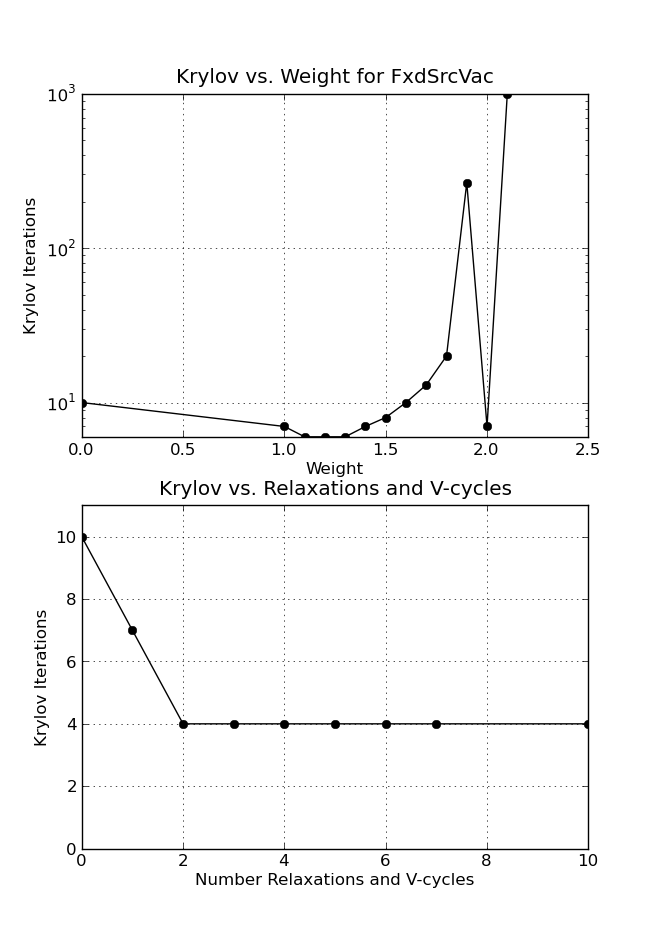
\includegraphics [width=0.7\textwidth, height=0.8\textheight] {FxdSrcVac}
   \end{center}
   \caption{Small Fixed Source Problem with Vacuum Boundaries, Preconditioning Parameter Studies}
   \label{fig:FxdSrcVac}
\end{figure}

Next the number of relaxations per grid and the number of V-cycles were varied with the weight fixed at 1. These results are shown in the bottom plot of Figure~\ref{fig:FxdSrcVac}. Here $r$ and $v$ were changed together, so the number on the x-axis represents both parameters. That is, if the x-axis value is 3 then $r$ and $v$ were both 3. 

Initially, increasing $r$ and $v$ reduced the number of iterations needed for convergence. After enough preconditioning was done that only 4 iterations were needed, no additional amount of preconditioning reduced the iteration count further. The data from this plot is in Appendix~\ref{sec:AppendixD}, Table~\ref{table:FxdSrcTstVacRV}. 

A calculation using $w1.3r10v10$, the largest set of preconditioning parameters tested, also yielded 4 iterations. This both confirms that more preconditioning did not improve results, and demonstrated that a lot of preconditioning did not cause breakdown. 

%-------------------------------------------------------------------------------------------------------
The previous problem was repeated with reflecting boundary conditions, and both a weight variation and $r$/$v$  variation study were done. This time the tolerance and upscatter tolerance were 1 $\times$ 10$^{-6}$. A plot of results for varying the weight with 1 relaxation per level and 1 V-cycle is in the top of Figure~\ref{fig:FxdSrcRefl}. The results for varying with number of relaxations per grid and the number of V-cycles with the weight fixed at 1 can be seen in the bottom plot. A few $r$/$v$ variations were also done using a weight of 1.3, indicated by large green dots.
%
\begin{figure}[!ht]
    \begin{center}
      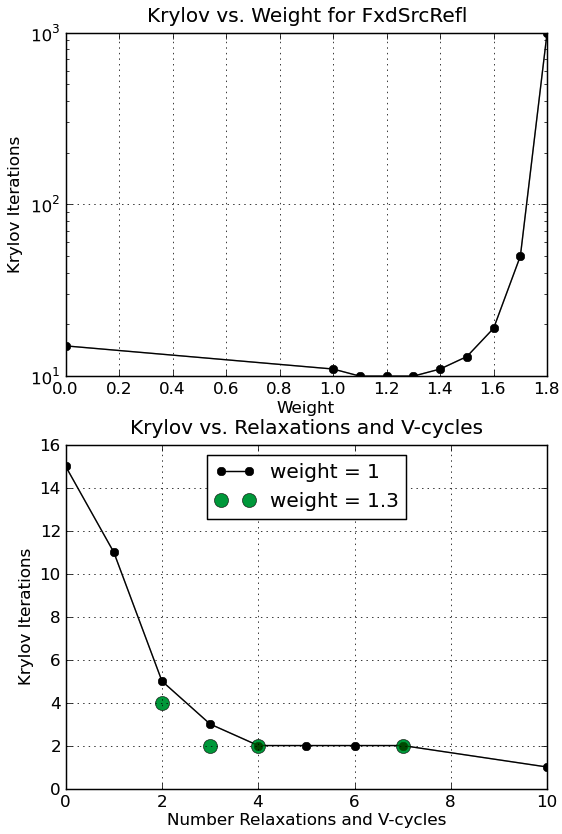
\includegraphics [width=0.7\textwidth, height=0.8\textheight] {FxdSrcRefl}
   \end{center}
   \caption{Small Fixed Source Problem with Reflecting Boundaries, Preconditioning Parameter Studies}
   \label{fig:FxdSrcRefl}
\end{figure}

The behavior of this problem was similar to but slightly different from the vacuum case. Increasing the weight parameter again decreased the number of iterations initially, and increased the number with higher $w$s. This behavior is different from what was observed in the RQI unit test reflecting case where increased weight always had a negative impact. For this test there was no ``sweet spot'' as in the vacuum case, and 1,000 iterations was reached at $w1.8$ rather than $w2.1$.

The $r$ and $v$ study showed two new things compared to the vacuum case. One is that early on a higher weight of 1.3 was better than a weight of 1. The other was that the number of iterations could be decreased to 1 when a large amount of preconditioning was done. Whether and when 1 iteration can be reached for a given problem is related to how well Richardson iteration works for that problem's characteristics. 

These two sets of results confirm that increasing $r$ and/or $v$ decreases Krylov iteration count. They also indicate that using a small amount of weight can be beneficial, but a large amount is not. Neither of these problems exhibited the problems with a weight over 1 at low $r$ and $v$. However, all of the tests discussed so far were very small and simple. Testing with larger and more complex problems is needed as well. 

%-------------------------------------------------------------------------------------------------------
%-------------------------------------------------------------------------------------------------------
\subsection{Fixed Source Solver and Angle Comparisons} 
Another fixed source problem was the half iron, half graphite cube from Chapter~\ref{sec:Chp2}. For this calculation a grid of 10 $\times$ 10 $\times$ 10 was used with an $S_{8}$ angle set. The tolerance and upscatter tolerance were 1 $\times$ 10$^{-6}$. This problem has vacuum boundaries and 27 energy groups, 13 of which have upscattering. A few calculations were done with this configuration to compare one set of preconditioning parameters to a few solvers without preconditioning. The solver comparisons can be seen in Table~\ref{table:FeC solvers} (note, the first three values in this table were shown in Chapter \ref{sec:Chp2}). The last column in the table shows the ratio of the case of interest's time to the MG Krylov time to provide a better sense of how the times compare to one another.
%
\begin{table}[!h]
\caption{Iron Graphite Fixed Source Cube, Solver and Preconditioning Comparison}
\begin{center}
\begin{tabular}{| l | c | l | c | c |}
\hline
Solver & GS Iters & Krylov & Subspace Length & Rel Time$^{*}$\\[0.5ex]
\hline
GS &  12 & 1,727 & 1 group & 2.41 \\ %$2.12 \times 10^{2}$
GS TTG & 11 & 1,687 & 1 group & 2.27 \\ %$1.99 \times 10^{2}$
MG Krylov & n/a & 30 & 27 groups & 1.00 \\ %$8.78 \times 10^{1}$
w1 r2 v2 & n/a & 10 & 27 groups & 8.05 \\ %$7.07 \times 10^{2}$
w1.3 r4 v4 & n/a & 4 & 27 groups & 14.68 \\ %$1.29 \times 10^{3}$
\hline
\end{tabular}\\
$^{*}$compared to unpreconditioned MG Krylov, 87.8 seconds
\end{center}
\label{table:FeC solvers}
\end{table}

All of the calculations using the block Krylov solver dramatically reduced the number of Krylov iterations for this problem, which contains highly scattering material. While the Krylov subspace sizes are made from smaller vectors when GS is used, all the problems using MG Krylov took many fewer iterations. The preconditioner also had a big impact. The highly preconditioned problem needed 4 Krylov iterations while the unpreconditioned Krylov case took 30 and unaccelerated Gauss Seidel needed 1,727.  

The timing comparison is not as favorable. With the current unoptimized state of the preconditioner, using it for fixed source problems increases rather than decreases run time. Even though many fewer Krylov iterations are taken, the overall preconditioned run times are longer than all other calculations. 

This problem investigated the option of using a reduced angle set within the preconditioner. The preconditioning parameters were $w1r2v2$. The overall problem was solved with $S_{8}$, but the preconditioner used $S_{2}$. Changing the number of solution directions did not change the number of iterations. The solution time was reduced from $7.07 \times 10^{2}$ seconds to $1.57 \times 10^{2}$ seconds, a factor of 4.5. The relative time is 1.79. With this option the solve time was less than both GS cases and approaching the unpreconditioned MG Krylov case. Using fewer solve directions inside the preconditioner had a very positive impact; it reduced time but did not impact the number of iterations.

%-------------------------------------------------------------------------------------------------------
%-------------------------------------------------------------------------------------------------------
\subsection{RQI Intermediate Problem}
The intermediate-size infinite medium problem from Chapter~\ref{sec:Chp3} that has 27 groups and a very small dominance ratio was solved with preconditioned RQI. This was the first system that tested if the preconditioner can converge the Krylov iterations when they did not converge without it. Recall that originally RQI got an eigenvalue close to the correct answer, but was unable to converge the eigenvector. For this test both $k$ and the flux were compared to a reference solution. Like all the problems discussed so far, this was solved without any parallelization using GMRES and the debug version of Denovo. 

\begin{table}[!h]
\caption{Infinite Medium Eigenvalue Problem, Preconditioning Results with Rayleigh Quotient Iteration}
\begin{center}
\begin{tabular}{| c | c | c | c | l | c | c | c | c |}
\hline
$w$ & $r$ & $v$ & $k$ & Krylov & RQI & Max Rel Diff & RMS Err & Rel Time$^{+}$ \\[0.5ex]
\hline
0    & 0 & 0 & 0.3970 & 39,025              & 40$^{*}$  & n/a & n/a & 211.03 \\%$5.43 \times 10^{4}$ \\
1    & 1 & 1 & 0.3982 & 3,014$^{\dag}$ & 4 & $1.67 \times 10^{-1}$ & $3.32 \times 10^{-2}$ & 103.56 \\%$2.66 \times 10^{4}$ \\
1    & 3 & 1 & 0.3983 & 50                     & 3 & 0.0 & 0.0 & 40.19 \\ %$1.03 \times 10^{4}$ \\
1    & 4 & 1 & 0.3983 & 44$^{\dag}$      & 3 & 0.0 & 0.0 & 4.51 \\ %$1.16 \times 10^{3}$ \\
1    & 2 & 2 & 0.3983 & 44$^{\dag}$      & 3 & 0.0 & 0.0 & 1.11 \\ %$2.86 \times 10^{2}$ \\
1    & 4 & 4 & 0.4001 & 16                     & 3 & $1.67 \times 10^{-1}$ & $3.21 \times 10^{-2}$ & 7.73 \\ %$1.99 \times 10^{3}$ \\
1    & 5 & 4 & 0.4001 & 14$^{\dag}$     & 3 & $1.67 \times 10^{-1}$ & $3.21 \times 10^{-2}$ & 8.81 \\ %$2.27 \times 10^{2}$ \\
1.4 & 5 & 4 & -0.4711 & 12$^{\dag}$    & 2 & $1.67 \times 10^{-1}$ & $3.21 \times 10^{-2}$ & 6.77 \\ %$1.74 \times 10^{3}$ \\
1    & 5 & 5 & -0.4575 & 7$^{\dag}$      & 2 & $3.43 \times 10^{-6}$ & $3.67 \times 10^{-5}$ & 6.13 \\ %$1.58 \times 10^{3}$ \\
\hline
1.1 & 4 & 1 & 0.3983 & 43$^{\dag}$      & 3 & 0.0 & 0.0 & 4.51 \\ %$1.16 \times 10^{3}$ \\
1.1 & 1 & 4 & 0.3983 & 43$^{\dag}$      & 3 & 0.0 & 0.0 & 5.24 \\ %$1.35 \times 10^{3}$ \\
1.1 & 2 & 2 & 0.3983 & 43$^{\dag}$      & 3 & 0.0 & 0.0 & 4.57 \\ %$1.18 \times 10^{3}$ \\
\hline
0.7 & 1 & 1 & 0.3999 & 3,001$^{\dag}$ & 4 & 1.0 & $3.72 \times 10^{-1}$ & 87.34 \\ %$2.25 \times 10^{4}$ \\
0.7 & 3 & 1 & 0.4001 & 87$^{\dag}$      & 5 & 0.0 & 0.0 & 7.60 \\ %$1.95 \times 10^{3}$ \\
0.7 & 3 & 3 & 0.4001 & 47$^{\dag}$      & 5 & 0.0 & 0.0 & 11.34 \\ %$2.92 \times 10^{3}$ \\
0.4 & 3 & 1 & 0.4001 & 1,052$^{\dag}$ & 4 & $1.18 \times 10^{-5}$ & $8.43 \times 10^{-8}$      & 67.57 \\ %$1.74 \times 10^{4}$ \\
\hline 
\end{tabular}\\
$^{+}$compared to unpreconditioned PI, $2.57 \times 10^{2}$ seconds\\
$^{*}$terminated manually\\
$^{\dag}$negative flux
\end{center}
\label{table:impi RQI}
\end{table}
%
The preconditioned results are shown in Table~\ref{table:impi RQI}. In the table ``Max Rel Diff'' is the maximum over all cells and all groups of the relative difference between the reference flux and the absolute value of the computed flux, $\max[ (\phi_{ref} - \vert\phi_{calc}\vert) / \phi_{ref}]$. ``RMS Err'' is the root mean squared (rms) relative error, $\sqrt{ \sum_{1}^{N}(rel\_err)^{2} / N}$. As a reminder, the total and upscattering tolerances were $1 \times 10^{-4}$, and the $k$ tolerance was $1 \times 10^{-5}$. Recall that if the Krylov iteration count is in the thousands it means the eigenvector did not converge in every iteration. The ``Rel Time'' column is the ratio of the found time to the unpreconditioned PI time of $2.57 \times 10^{-2}$ seconds.

Two pieces of information are pertinent for interpreting these results. One is that when a calculation is terminated manually, the flux information is not reported since the calculation does not go through post-processing. This means that for the unpreconditioned case it is only known that the flux did not converge, not whether the flux was positive or negative, nor how far the estimate at termination was from the reference solution. Recall that Denovo terminates if a negative eigenvalue is computed. For the two cases in which a negative eigenvalue is reported it simply means a negative $k$ was computed on iteration 2, not that the problem converged in 2 RQ iterations. 

This calculation performed strangely when preconditioned, though the results were not necessarily worse than when it was not. A wide variety of preconditioning parameter combinations were tried and there were zero out of fifteen cases that exactly matched the reference eigenpair. 

Of the thirteen cases where the eigenvector converged in every iteration, the flux was completely correct in one and correct in magnitude but negative in seven. There were two cases, $w1r5v5$ and $w0.4r3v1$, where the absolute value of the flux did not match the reference exactly but was within the convergence tolerance. The first of these terminated before convergence because of a negative eigenvalue, and the second had one set of Krylov iterations that did not converge. In the remaining cases there was a real difference between the found and reference eigenvectors, even though the eigenvectors and values converged. 

Another important issue was that the correct eigenvalue of 0.40031 was never found within $1 \times 10^{-5}$, even when the flux matched the reference exactly. The reported eigenvalues differ from the reference by between $2.03 \times 10^{-4}$ and $2.03 \times 10^{-3}$, excluding the negative $k$ and unconverged Krylov cases. Because the converged-upon $k$ is farther from the reference than the $k$ tolerance, the method is converging to the wrong value. 

These behaviors bring up some serious concerns. One is that the method gives no warning or indication that something has gone awry until a negative eigenvector/value is reported at the end of the calculation. Another is that in one case the flux matched the reference exactly, but $k$ did not. Finally, that the problem can converge to the wrong $k$ is disconcerting. Note that none of these behaviors were observed in any other test cases.  

To investigate whether some of the strange behavior was coming from GMRES, this problem was also attempted with BiCGSTAB. The preconditioning was set to $r2v2$, and the weight was increased in 0.1 increments from 1.0 to 1.5. In the cases where the calculation terminated itself; $w1.0$, $w1.4$, $w1.5$; it was because a negative eigenvalue was found. Those eigenpairs were incorrect. 

In the other cases; $w1.1$, $w1.2$, $w1.3$; the problems were terminated manually. At termination, the eigenvalue was oscillating between a number close to the correct answer and a large number like 11. The flux was not printed for the manually terminated cases, so it is unknown whether the flux was correct or not. Not only did BiCGSTAB not improve the results, it performed worse than GMRES.

This intermediate problem was also solved with power iteration using no preconditioning and using a lot of preconditioning. Without preconditioning the problem took 180 Krylov iterations and $2.57 \times 10^{2}$ seconds. With $w1r5v5$ preconditioning it took 12 Krylov iterations and $2.19 \times 10^{3}$ seconds. Both calculations obtained an eigenvalue and flux within the reference solutions. Preconditioning substantially reduced the number of Krylov iterations needed. Further, power iteration got the right answer when RQI did not. 

At this time it is unknown why preconditioned RQI had such a hard time with this calculation. Preconditioned RQI did have more trouble with the small reflecting problem than the vacuum problem, and this test had all reflecting boundaries. Perhaps the characteristics of $\ve{A}$ for this problem are quite difficult for RQI. Whatever the reason, RQI did not perform well on this problem regardless of whether it was preconditioned.  

Some parameter information can still be gleaned from this study. The eigenvector did not converge after the first iteration when $r1v1$ was used with either $w1$ or $w0.7$. With more preconditioning the problem converged and the number of both RQI and Krylov iterations was reduced. This is similar to what has been seen before. However, when a lot of preconditioning was used, the problem calculated a negative eigenvalue. This is a behavior that was not observed in the simpler problems. 

These numbers further confirm that it is the total number of relaxations done, not the specific combination of $r$ and $v$, that determine the reduction in iteration count. That is, iteration count with $r4v1$ is the same as with $r2v2$ and $r1v4$; though there is a difference in timing. The way the $r4v1$ and $r2v2$ times differ from one another is not the same between $w1$ and $w1.1$. This suggests these timing numbers may not be reliable, which was expected because these calculations were not done on a machine dedicated to their computation.

%-------------------------------------------------------------------------------------------------------
%-------------------------------------------------------------------------------------------------------
\subsection{2-D C5G7 Benchmark Study}
Next, the preconditioner was applied to the 2-D C5G7 benchmark using both PI and RQI with the goals of seeing if preconditioned RQI could converge the flux and $k$, to investigate the effect of preconditioning in both RQI and PI, and to see whether the lessons learned about preconditioning parameters still hold in a real problem. The calculation used 16 cores on the small orthanc cluster at Oak Ridge: 4 $x$-blocks, 4 $y$-blocks, 1 $z$-block and 1 energy set. The total and upscattering tolerances were $1 \times 10^{-3}$, with a $k$ tolerance of $1 \times 10^{-5}$. An optimized version of Denovo was used.  

A weight variation study was done with power iteration first. The results using $r1v1$ are plotted as Krylov Iterations vs.\ Weight, and Time in seconds vs.\ Weight in Figure~\ref{fig:2-Dc5g7PI}. The data that is plotted can be found in Appendix~\ref{sec:AppendixD}, Table~\ref{table:2-D c5g7}. All calculated $k$s were within the uncertainty of the benchmark and so are not reported. All preconditioned cases needed 31 power iterations while the unpreconditioned case took 32.
%
\begin{figure}[!ht]
    \begin{center}
      \includegraphics [width=0.7\textwidth, height=0.7\textheight] {2dc5g7PI}
   \end{center}
   \caption{2-D C5G7 Benchmark, Preconditioner Weight Variation with Power Iteration}
   \label{fig:2-Dc5g7PI}
\end{figure}

This study shows the preconditioner is very effective at reducing the number of Krylov iterations used by power iteration. The unpreconditioned case, corresponding to a weight of 0 on the plot, took 3,129 MG Krylov iterations. As the weight was increased from 1 to 1.4, the number of Krylov iterations and the time to solution both decreased. With $w1.4$, 1,458 MG Krylovs were taken. The time and iteration count both went back up with a weight of 1.5. When the weight was increased beyond 1.5 none of the multigroup iterations converged, and the problem was terminated manually after several power iterations. 

Two other calculations with a higher level of preconditioning were also done. When the parameters were $w1.4r2v2$ the number of Krylov iterations were reduced to 438 and the calculation took $1.77 \times 10^{4}$ seconds, both lower than all the cases using $r1v1$. For $w1r3v3$, 253 Krylov iterations and $2.28 \times 10^{4}$ seconds were required. This had the smallest number of Krylov iterations, but a slightly longer time than all the calculations except $w1.5r1v1$.	

The results from the RQI study are in Table~\ref{table:2-D c5g7 rqi}. In all cases, except the unpreconditioned one, $k$ was within the uncertainty of the benchmark value. The ``$<$ 1,000?'' column indicates whether or not the multigroup iterations converged during the RQI process. If the value is ``no'' that means the eigenvector only converged during the first iteration. A number indicates the last eigenvalue iteration for which the Krylov method took less than 1,000 iterations. All subsequent iterations required the full 1,000. A ``yes'' means all of the Krylov iterations converged. The relative time is the ratio of the case of interest to the unpreconditioned PI time of $8.54 \times 10^{3}$ seconds.
%
\begin{table}[!h]
\caption{2-D C5G7 Benchmark, Convergence Study with Rayleigh Quotient Iteration}
\begin{center}
\begin{tabular}{| c | c | c | l | c | c | c |}
\hline
Weight & Relaxations & V-cycles & Krylov & RQI & $<$ 1,000? & Rel Time$^{\dag}$\\[0.5ex]
\hline
0    & 0 & 0 & 119,006 & 120$^{*}$ & no & 10.98 \\%$9.38 \times 10^{4}$ \\
1    & 1 & 1 & 16,007   & 17            & no & 23.65 \\ %$2.02 \times 10^{5}$ \\
1.2 & 1 & 1 & 40,008   & 41$^{*}$   & no & 13.00 \\ %$2.06 \times 10^{5}$ \\
1    & 3 & 1 & n/a         & n/a$^{*}$  & 7   & n/a \\
1    & 2 & 2 & 11,158   & 19            & alternated & 46.72 \\ %$3.99 \times 10^{5}$ \\
1    & 3 & 2 & 3,320     & 19            & 14 &19.23 \\ % $1.64 \times 10^{5}$ \\
\hline
1    & 3 & 3 & 299        & 19            & yes & 3.01 \\ %$2.57 \times 10^{4}$ \\
1.1 & 3 & 3 & 281        & 19            & yes & 2.80 \\ %$2.40 \times 10^{4}$ \\
1.3 & 3 & 3 & 254        & 19            & yes & 2.57 \\ %$2.19 \times 10^{4}$ \\
1.5 & 3 & 3 & n/a         & n/a$^{*}$ & no & n/a \\
\hline 
\end{tabular} \\
$^{\dag}$compared to unpreconditioned PI, $8.54 \times 10^{3}$ seconds\\
$^{*}$terminated manually
\end{center}
\label{table:2-D c5g7 rqi}
\end{table}
%

These results show a few important things. Most significantly, with enough preconditioning the multigroup iterations within RQI can be converged and the right eigenpair can be found. For the first three $w\#r3v3$ cases all of the Krylov iterations converged. In these cases the calculation time decreased by an order of magnitude compared to the ones where they did not converge every time because so many fewer eigenvalue iterations were needed. This test case was the first to demonstrate that the preconditioner can get RQI to converge. 

For many of the calculations the eigenvector did not converge or did not converge all the time, but the correct eigenvalue was still found (even in the $w1.2r1v1$ case that was terminated manually). As the preconditioning increased, the eigenvector came closer to converging for all iterations. When the Krylov iterations converged, increasing the weight decreased iteration count and wall time for small weights. As in other tests, too much weight caused the calculation not to converge at all. 

Additionally, it seems that preconditioning held RQI on track enough to get the right eigenvalue when the eigenvector did not quite converge. As was hypothesized for the unpreconditioned infinite medium test, it may be that the eigenvector was close enough to correct that a good approximation to the eigenvalue could still be made from it, even though the vector itself did not converge. 

Only the $w1r3v3$ calculation overlaped between RQI and PI. PI took fewer Krylov iterations, 253 compared to 299, and less time, $2.28 \times 10^{4}$ compared to $2.57 \times 10^{4}$ seconds. For this test preconditioned RQI did not perform as well as preconditioned PI, though the times and iteration counts were close to one another. 

From the standpoint of comparing eigenvalue solution methods, it is worth noting that RQI required 19 eigenvalue iterations while PI required 31. Both methods use eigenvectors from the inside multigroup solves to compute eigenvalues in the outer iterations. When given eigenvectors that have been converged to the same tolerance, RQI needed fewer eigenvalue iterations than PI. In this case it took more Krylov iterations within each multigroup solve to get the eigenvector to that tolerance, so RQI was not better in terms of total Krylov count.

The RQI problem was also tried with BiCGSTAB as the Krylov solver for an unpreconditioned case and a $w1r3v3$ case. Every multigroup iteration went to the 1,000 iteration limit and the problem was terminated manually after several RQ iterations.

%-------------------------------------------------------------------------------------------------------
%-------------------------------------------------------------------------------------------------------
 \subsection{3-D C5G7 Benchmark Study}
The preconditioner using both PI and RQI was also applied to the 3-D C5G7 benchmark with an optimized version of Denovo. The goals of this study were essentially the same as the 2-D study, except that this problem is larger, and the first to approach a real ``grand challenge'' type of calculation. The medium-sized oic cluster at Oak Ridge was used and each problem was given 720 cores with 40 $x$-blocks, 18 $y$-blocks, and 5 $z$-blocks. The total and upscattering tolerances were $1 \times 10^{-4}$, with a $k$ tolerance of $1 \times 10^{-5}$ unless otherwise indicated. The wall time limit was 12 hours. 

The power iteration results are in Table~\ref{table:3-D c5g7}. The relative time is compared to unpreconditioned PI, $4.46 \times 10^{3}$ seconds. The unpreconditioned power iteration calculation computed a $k$ that was not within the uncertainty bounds of the reported benchmark; it was low by about 0.011. All preconditioned PI and RQI tests computed a $k$ that was within the Denovo $k$ tolerance of the unpreconditioned PI result so they are not reported here. Subsequent to these calculations it was determined that using a more accurate quadrature gives the correct $k$. 
%
\begin{table}[!h]
\caption{3-D C5G7 Benchmark, Preconditioning Parameter Scoping with Power Iteration}
\begin{center}
\begin{tabular}{| c | c | c | c | l | c |}
\hline
Weight & Relaxations & V-cycles & Krylov & PI & Rel Time$^{\dag}$ \\[0.5ex]
\hline
0    & 0 & 0 & 1,224 & 32 & 1.00 \\ %$4.46 \times 10^{3}$ \\
1    & 1 & 1 & 708    & 32 & 5.90 \\ %$2.12 \times 10^{4}$ \\
1.2 & 1 & 2 & 448    & 32 & 5.33 \\ %$2.38 \times 10^{4}$ \\
1.2 & 2 & 1 & 448    & 32 & 5.37 \\ %$2.39 \times 10^{4}$ \\
1.3 & 2 & 2 & 288    & 32 & 6.37 \\ %$2.84 \times 10^{4}$ \\
1    & 3 & 3 & 126    & 14$^{*}$  & 9.05 \\ %$4.04 \times 10^{4}$ \\
1.5 & 3 & 3 & 192    & 32 & 8.36 \\ %$3.73 \times 10^{4}$ \\
1    & 4 & 4 & n/a     & n/a          & exceeded wall time \\
1    & 4 & 4 & n/a     & n/a$^{*}$ & exceeded wall time \\
1.5 & 5 & 5 & n/a     & n/a          & exceeded wall time \\
\hline 
\end{tabular}\\
$^{\dag}$compared to unpreconditioned PI, $4.46 \times 10^{3}$ seconds\\
$^{*}$tol and upscatter tol = $1 \times 10^{-5}$, $k$ tol = $1 \times 10^{-3}$
\end{center}
\label{table:3-D c5g7}
\end{table}

The 3-D benchmark study shows the preconditioner with PI can reduce the number of required Krylov iterations substantially for challenging problems. The number of eigenvalue iterations for a given tolerance set were never changed by preconditioning. 

The effect of preconditioning parameters was consistent with what was observed in other test problems. However, using large values for $r$ and $v$ made the calculation take too long to get results. On the oic machine, if a calculation exceeds wall time there is no way to get any of the results from the scratch space. Therefore, no conclusions can be drawn from this problem about the effect of substantial preconditioning when using power iteration for a real, 3-D problem. 

The RQI results are in Table~\ref{table:3-D c5g7 rqi}. The relative time is compared to unpreconditioned PI, $4.46 \times 10^{3}$ seconds. Many cases did not finish in time to report results. What is likely happening when the problems with lower parameter values run out of time is that the eigenvector is not converging. As was seen before, the calculations take a long time when every eigenvalue iteration uses 1,000 Krylov iterations. Unfortunately, there is no way to confirm this theory or find out if the eigenvalue is close to correct since the output cannot be obtained. 
%
\begin{table}[!h]
\caption{3-D C5G7 Benchmark, Preconditioning Parameter Scoping with Rayleigh Quotient Iteration}
\begin{center}
\begin{tabular}{| c | c | c | c | l | c |}
\hline
Weight & Relaxations & V-cycles & Krylov & RQI & Rel Time$^{+}$ \\[0.5ex]
\hline
0    & 0 & 0 & n/a     & n/a          & exceeded wall time \\
1    & 1 & 1 & n/a     & n/a          & exceeded wall time \\
1.5 & 1 & 1 & n/a     & n/a          & exceeded wall time \\
1.2 & 2 & 1 & n/a     & n/a          & exceeded wall time \\
1.3 & 2 & 2 & 302    & 19           & 5.20 \\ %$2.32 \times 10^{4}$ \\
1    & 3 & 3 & 103    & 9$^{*}$    & 6.67 \\ %$3.02 \times 10^{4}$ \\
1    & 3 & 3 & 164    & 15$^{\dag}$ & 7.59 \\ %$3.38 \times 10^{4}$ \\
1.5 & 3 & 3 & 187    & 19           & 7.26 \\ %$3.24 \times 10^{4}$ \\
1    & 4 & 4 & n/a     & n/a          & exceeded wall time \\
1    & 4 & 4 & 74     & 9$^{*}$    & 5.13 \\ %$2.29 \times 10^{4}$ \\
1.5 & 5 & 5 & n/a     & n/a          & exceeded wall time \\
\hline 
\end{tabular}\\
$^{+}$compared to unpreconditioned PI, $4.46 \times 10^{3}$ seconds\\
$^{*}$tol and upscatter tol = $1 \times 10^{-5}$, $k$ tol = $1 \times 10^{-3}$\\
$^{\dag}$tol and upscatter tol = $1 \times 10^{-4}$, $k$ tol = $5 \times 10^{-5}$
\end{center}
\label{table:3-D c5g7 rqi}
\end{table}  

With an intermediate amount of preconditioning, RQI converged and performed better than the analogous PI cases. There are three cases where both problems finish and the same tolerances were used: $w1.3r2v2$, $w1r3v3$, $w1.5r3v3$. These results are shown together in Table~\ref{table:PI RQI} for ease of comparison. This table displays time instead of relative time since the comparison is between two cases rather than across all cases. In all three the RQI calculations took less time and fewer eigenvalue iterations than PI. In the second two they also took fewer Krylov iterations. RQI even finished in time to get results from the $w1r4v4$ calculation when PI did not. 
%
\begin{table}[!h]
\caption{3-D C5G7 Benchmark, Rayleigh Quotient Iteration and Power Iteration Comparison}
\begin{center}
\begin{tabular}{| c | c | c | c | c | c | c |}
\hline
Sovler & Weight & Relaxations & V-cycles & Krylov & Eigenvalue & Time (s) \\[0.5ex]
\hline
RQI & 1.3 & 2 & 2 & 302    & 19           & $2.32 \times 10^{4}$ \\
PI    & 1.3 & 2 & 2 & 288    & 32           & $2.84 \times 10^{4}$ \\
RQI & 1    & 3 & 3 & 103    & 9$^{*}$   & $3.02 \times 10^{4}$ \\
PI    & 1    & 3 & 3 & 126    & 14$^{*}$ & $4.04 \times 10^{4}$ \\
RQI & 1.5 & 3 & 3 & 187    & 19           & $3.24 \times 10^{4}$ \\
PI    & 1.5 & 3 & 3 & 192    & 32           & $3.73 \times 10^{4}$ \\
\hline 
\end{tabular}\\
$^{*}$tol and upscatter tol = $1 \times 10^{-5}$, $k$ tol = $1 \times 10^{-3}$
\end{center}
\label{table:PI RQI}
\end{table}  

The 3-D benchmark problem shows that for at least some problems, preconditioned RQI converges more quickly in all senses than preconditioned PI. It is pertinent that this is true is the most interesting problem shown so far. It seems, however, that RQI can only be useful if it is preconditioned enough to get the eigenvector to converge. 

These results continue to confirm that a small amount of weight works well for real problems. Increasing $r$ and $v$ decrease iteration count, but at what can be a high time penalty. An intermediate amount of preconditioning will likely provide the best balance of reduced iteration count for the time invested once the preconditioner is optimized. 

%-------------------------------------------------------------------------------------------------------
%-------------------------------------------------------------------------------------------------------
\subsection{Multisets}
Another important area of investigation was how the preconditioner faired when using multisets. To investigate the effect of multigrid in energy with multisets on the Krylov iterations without worrying about impacts of an eigenvalue calculation, the iron graphite fixed source problem was considered first. These data were calculated on orthanc using an optimized version of the code. All previous parameter studies were used to pick preconditioning values that were likely to work well. 

For this study the spatial grid was increased to $50 \times 50 \times 50$ and $S_{4}$ was used instead of $S_{8}$. The unpreconditioned version was compared to one with $w1r2v2$ on 1 to 10 sets. Note that with 27 groups, 10 sets was the maximum possible to still be able to use the preconditioner. In addition, 2 $x$-blocks, 2 $y$-blocks, and 1 $z$-block were used. The calculations were therefore done on between 4 and 40 cores. The preconditioned calculation took 27 GMRES iterations while the unpreconditioned took 123 regardless of the number of sets used.

Because the number of iterations did not change with sets, the only thing to compare is time. The focus is on relative change in time rather than absolute time since there is still room for the preconditioner to be optimized. All times in this section include the improved multiset communication strategy that was described at the end of Chapter~\ref{sec:Chp2}. 

Three plots are shown in Figure~\ref{fig:FeC multisets}. From the top, the first shows the wall time for the preconditioned and unpreconditioned (``regular'') calculations as a function of number of energy sets. The second plots the efficiency of the regular and preconditioned tests, where the base case is 1 set. The last plot is of the relative difference between the two times. The data that are plotted can be found in Appendix~\ref{sec:AppendixD}, Table~\ref{table:FeC multisets}.
%
\begin{figure}[!ht]
    \begin{center}
      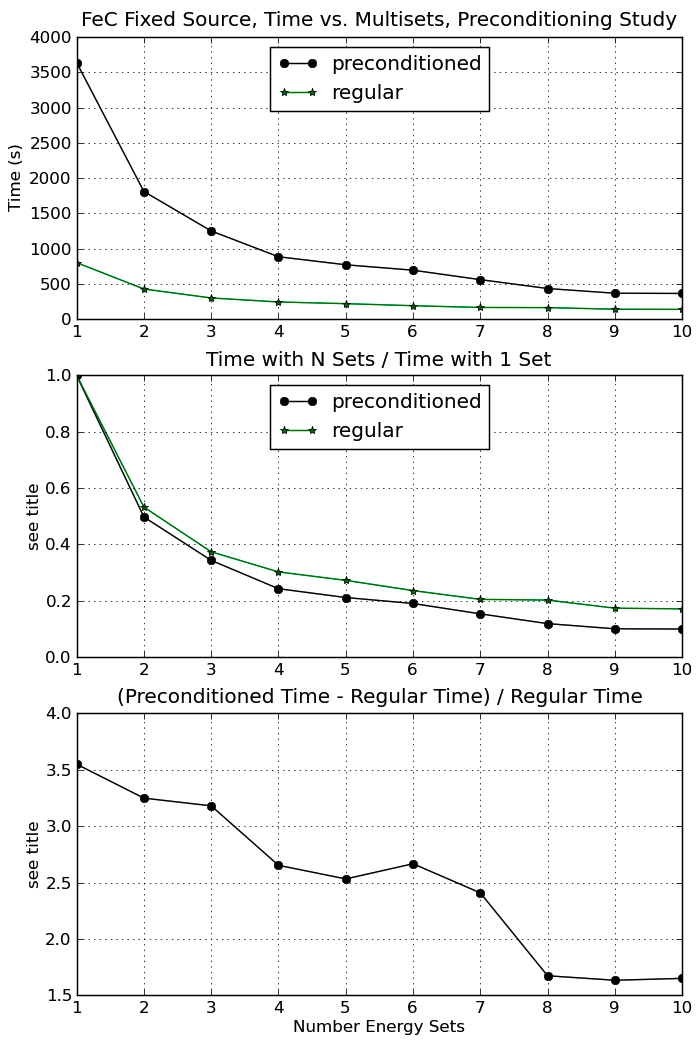
\includegraphics [width=0.67\textwidth, height=0.85\textheight] {FeCmultisets}
   \end{center}
   \caption{Iron Graphite Fixed Source Problem, Preconditioned Multiset Study}
   \label{fig:FeC multisets}
\end{figure}

The 1 set wall time without preconditioning was $8.00 \times 10^{2}$ seconds and the 10 set time was $1.37 \times 10^{2}$ seconds. Another way to say this is that the 1 set time took about 6 times longer to run than the 10 set time. If the problem scaled linearly in energy, it would have taken 10 times longer. The unpreconditioned efficiency degraded slowly with increasing energy sets, and the efficiency with 10 sets was less than 60\%.

With preconditioning the 1 set time was $3.64 \times 10^{3}$ and the 10 set time was $3.63 \times 10^{2}$. Going from 1 to 10 sets in this case was linear. The efficiency changed a bit with the number of energy sets, but ranged between about 90\% and 110\%. Thus for some sets the preconditioned case gave better than linear speedup. While the exact efficiencies may not be accurate because of timing variability, the general trends are clear. 

What the difference between the efficiencies in the preconditioned and regular tests means is that the preconditioned tests were accelerated more by using multisets than the unpreconditioned tests. As a result the preconditioned times approached the regular times as more sets were used. This can be seen in the bottom plot of relative difference between the times. 

Before more results with similar trends are shown, some reasons for the preconditioner's super-linear scaling in energy should be discussed. As the number of sets increases, each application of the preconditioner becomes less costly. The total preconditioning cost goes down because the V-cycle becomes shallower. That is, each application of the preconditioner is doing fewer total relaxations and is therefore less time intensive. This effect becomes more pronounced with larger $r$ and $v$. If the total number of Krylov iterations remains constant with sets, then there is no tradeoff and the preconditioner simply costs less with increased energy parallelization.

Another reason for the behavior is that this problem has a group structure that is not always balanced between sets. The multigrid preconditioner mitigates the penalty of energy set load imbalance. Recall that each set uses the same number of grids even if the groups per set are different. This means the work in the preconditioner is energy-load-balanced in all cases. Thus the relative amount of time spent waiting because of load imbalance decreases when the preconditioner is used. 

This test was also run with increased preconditioning parameters for 1 set and 10 sets to see if that made a difference. The angle set was changed back to $S_{8}$ and there was no decomposition in space. With $w1.3r4v4$ the number of Krylov iterations decreased to 11. With 1 set this took $6.49 \times 10^{4}$ seconds to complete. With 10 sets this was reduced to $5.02 \times 10^{3}$ seconds. A 10 fold increase in computing power gave nearly a 13 fold decrease in run time, or an efficiency of 129\%. 

Without preconditioning the 1 set wall time was $8.81 \times 10^{3}$ seconds and the 10 set time was $1.04 \times 10^{3}$ seconds. The ratio of 1 set to 10 set time was about 8.5, or 85\% efficient. This problem configuration scaled better than the previous configuration overall. The comparison between the preconditioned and unpreconditioned cases is similar. 

%-------------------------------------------------------------------------------------------------------
The infinite medium, 27 group problem was also used to study how the preconditioner faired with energy set decomposition. Because this problem has reflecting boundary conditions it could only be used with power iteration (recall, multisets are not implemented for RQI with reflecting boundaries at this time). These calculations were also done on orthanc, using between 1 and 10 sets and an optimized version of the code. No other problem settings were changed from what was presented above. 

Three plots comparing unpreconditioned PI and PI with $w1r2v2$ are shown in Figure~\ref{fig:impi multisets}. Each plot is of the same parameters as the corresponding plots in the iron graphite cube figure. A table of the data can be found in Appendix~\ref{sec:AppendixD}, Table~\ref{table:impi multisets}.
%
\begin{figure}[!ht]
    \begin{center}
      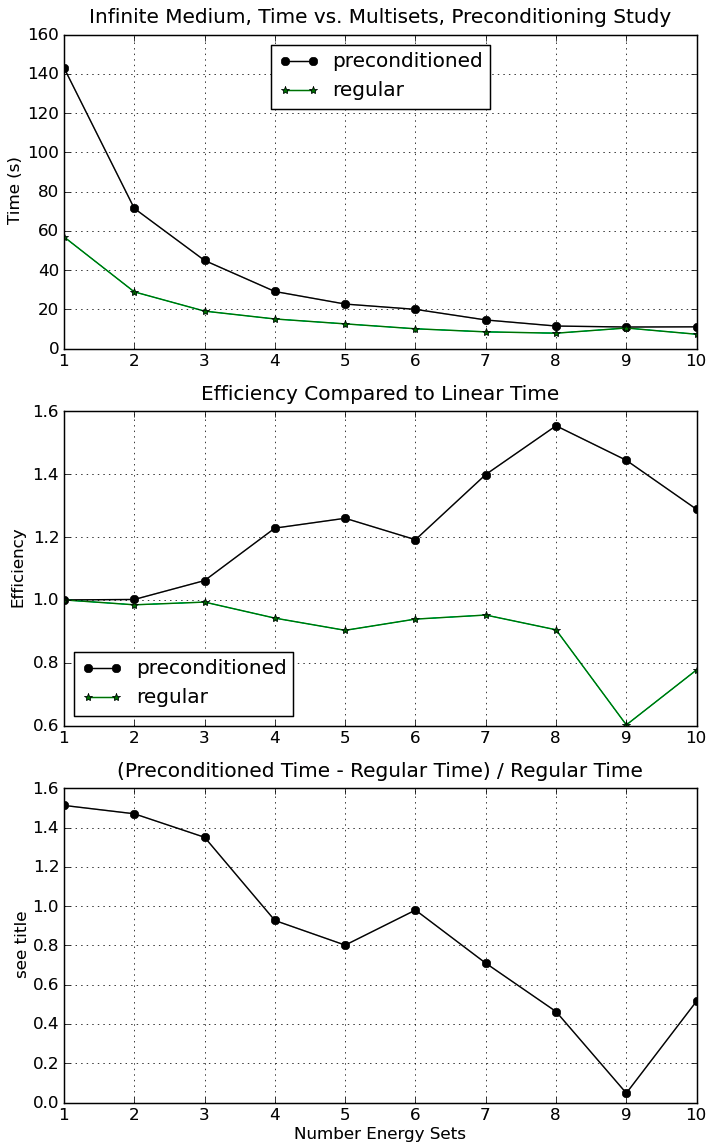
\includegraphics [width=0.67\textwidth, height=0.85\textheight] {impimultisets}
   \end{center}
   \caption{Infinite Medium Eigenvalue Problem, Preconditioned Multiset Study with Power Iteration}
   \label{fig:impi multisets}
\end{figure}

The infinite medium test with power iteration exhibited behavior similar to the fixed source test, though this problem scaled better in energy in general. With preconditioning the Krylov iterations were reduced from 180 (90 Krylov per PI with 2 PI) to 46 (23 Krylov per PI with 2 PI). Neither the number of Krylov nor eigenvalue iterations were changed by using more sets.  

%The preconditioned 1 set time was faster than the 10 set time by a factor of 12.9, while it was only 7.8 for the regular version. The preconditioned time was always at least linear, with the efficiency ranging from 1 to 1.55 and an average efficiency of 1.24. The regular efficiency was between 60\% and 99\%, with an average of 90\%. The relative difference between the preconditioned and regular times decreased from 1.51 with 1 set to 0.52 with 10 sets. These results show that the preconditioned results benefited more from multisets than the regular results, and the times approached one another as set count increased. 
This test was run with increased preconditioning parameters for 1 set and 10 sets as well. The number of Krylov iterations decreased to 8 per eigenvalue iteration, with 2 eigenvalue iterations when $w1r4v4$ was used. With 1 set this took $4.02 \times 10^{2}$ seconds to complete. With 10 sets this was reduced to $2.94 \times 10^{1}$ seconds. This preconditioning parameter set also performed very well, yielding a speedup of 13.7 for a 10 fold increase in computing power.  
 
A few key conclusions can be drawn from the multiset studies about the tradeoff between the number of groups per set and about the overall usefulness of the multigrid-in-energy method with multisets. An important observation is that the number of GMRES iterations did not change with the number of sets. This means convergence improvement from the preconditioner does not come from the depth of V-cycle. Only restricting down 1 or 2 grids had as much of an impact as restricting down something like 6. This indicates it is not necessary to coarsen down to one group. 

From an error mode reduction standpoint, this conclusion suggests what a Fourier expansion of the error in energy might look like. Because a few coarser grid had a large impact but many coarser grids did not, the bulk of the error might be intermediately oscillatory in energy. If the smooth error were dominant, then the coarsest grids would likely be necessary. Only solving on a fine grid, however, was not good enough, so the error is not only oscillatory either. This leaves the modes that are between the two extremes as the likely culprit for slow convergence. 

The super-linear energy scaling of the preconditioner warrants more discussion. Relaxing on the coarsest energy grids did not provide convergence benefit, meaning much work that was not beneficial was done when only a few sets were used. When many sets were used all of this work was eliminated without any negative consequences. Thus, the energy scaling was very good.

Once the preconditioner is optimized, the scaling in energy may not be as good since the preconditioner will take a smaller total fraction of the runtime. The scaling will also be less impressive if the preconditioner is modified to use only two or three grids all the time instead of always restricting down to one energy group. This would eliminate the un-beneficial work in all cases. 

Overall, the multigrid-in-energy method performed very well with multisets. After the modifications mentioned in the last paragraph are made, the preconditioner will likely no longer cause the entire calculation to scale so well in energy. However, the preconditioner does not communicate between sets and it does load-balance in energy. It therefore seem likely that the preconditioner can at worst leave the energy scaling behavior unchanged. 

\subsection{PWR Study}
Finally, the full-facility PWR problem was calculated on the Jaguar machine as the illustrative example of using all the new methods in combination. This test used the multigroup Krylov solver, the Rayleigh quotient iteration eigenvalue solver, and the parallelized multigrid-in-energy preconditioner. It is also exactly the kind of large and challenging problem this work is designed to solve. The PWR900 was solved with PI + MG Krylov + the multigrid-in-energy preconditioner as well. 

The 44-group, 1.7 trillion unknown version of the problem was used for this strong scaling study. The tolerance and $k$ tolerance were $1 \times 10^{-3}$, and the upscattering tolerance was $1 \times 10^{-4}$. The preconditioner settings were $w1r3v3$. 1, 4, 11, and 22 sets were used giving 44, 11, 4, and 2 groups per set and 8, 6, 4, and 2 energy grids, respectively. There were 578 $\times$ 578 $\times$ 700 mesh elements. With 22 sets, 96 $x$-blocks, 94 $y$-blocks, and 10 $z$-blocks were used. All other cases had 102 $x$-blocks, 100 $y$-blocks, and 10 $z$-blocks. The results using both eigenvalue solvers are in Table~\ref{table:full PWR}. 
%
\begin{table}[!h]
\caption{PWR900, Preconditioned Strong Scaling Study}
\begin{center}
\begin{tabular}{| l | c | c | c | l | c | c | l |}
\hline
Solver & Sets & Cores & $k$ & Krylov & Eigenvalue & Total (m) & Solver (m)\\[0.5ex]
\hline
RQI & 1   & 10,200   & 0.182 & 12    & 2$^{\dag}$ & 720.05    & n/a \\
%PI    & 1   & 10,200   &  &  &       &  &  \\
RQI & 4   & 40,800   & 1.269 & 76   &  6               & 802.60   & 801.32 \\
RQI w/ $S_{2}$ & 4   & 40,800   & 1.269 & 79   &  6               & 192.48   & 191.42 \\
PI    & 4   & 40,800   & 1.270 & 101 & 10$^{\dag}$ & 1440.12 & n/a \\
RQI & 11 & 112,200 & 1.269 & 76   & 6                & 331.43    & 330.38 \\
PI    & 11 & 112,200 & 1.270 & 111 & 11$^{\dag}$ & 480.63    & n/a \\
RQI & 22 & 198,528 & 1.269 & 76   & 6                & 143.62    & 142.56 \\
PI    & 22 & 198,528 & 1.271 & 161 & 16$^{*}$      & 285.92    & n/a \\
\hline 
\end{tabular}\\
$^{\dag}$exceeded wall time limit \\ 
$^{*}$machine taken down for maintenance during calculation
\end{center}
\label{table:full PWR}
\end{table}  

Based on the full PWR calculations done previously by Evans and Davidson, $k$ is approximately 1.27, though there were no results where the dominance ratio was reported. The previous calculations that used PI with the multigroup Krylov solver and multisets had looser tolerances than these tests, so $k$ is not known more accurately and timing comparisons are not valid. All of the calculations, even those that did not finish excluding the 1 set RQI case, found the correct $k$ compared to the accuracy with which it is known. 

Only RQI was used for the 1 set test. Jaguar limits problems using fewer than 20,000 cores to a 12 hour wall limit. Because the 4 set case took more than 12 hours it was not expected that the 1 set cases would finish. The test was still conducted to see whether the behavior of progress made toward solution differed from the multiset cases. That is, at eigenvalue iteration $x$ with 1 set were the $k$ and associated errors the same or different from those at iteration $x$ with a different number of sets. The purpose of this comparison was to see if the number of grid levels used in the preconditioner affected the iteration behavior. 

The 1 set RQI case had the same $k$ estimate and had done the same number of GMRES iterations as the 4, 11, and 22 set cases at iteration 2. Thus eight energy grid levels gave the same improvement as two energy grid levels at the outset of the calculation. Since the 1 set calculation did not finish it cannot be known if this trend would have held, though it seems likely. This behavior is consistent with what was found in the other two multiset studies, but of higher import since this was for a real problem.

RQI converged for 22, 11, and 4 sets. Changing the number of sets did not change the number of eigenvalue or eigenvector iterations for these cases. Neither an unpreconditioned calculation, nor one with different preconditioning parameters were tried. Nevertheless, these three tests show that the preconditioner can ensure that RQI converges both the eigenvalue and the multigroup iterations for a large, real problem. 

The ``RQI w/ $S_{2}$'' calculation used the reduced angle set option in the preconditioner. The overall calculation used $S_{12}$. Reducing that to $S_{2}$ within the preconditioner had a large impact, reducing the solver time from 13.36 to 3.19 hours, or 76\%. 

There were no cases where PI completed the calculation. Partway through the 22 set calculation a portion of the Jaguar machine was taken offline for maintenance leaving only 162,240 cores, so the calculation was terminated. The calculation cannot be completed because the machine will not be restored to the full 224,256 cores before this work must be submitted. 

The 11 and 4 set PI problems did not finish before the wall time limit was reached because the limit was not set high enough. Limits of 8 and 24 hours were chosen based on the RQI finish times of 5.5 and 13.4 hours, respectively. In previous problems the solve time for PI was close to or less than RQI, so the selected limits seemed reasonable. The 1 set case was not performed. It was determined that the additional information it might provide would not change any conclusions that can be made based on all of the other results. 

A true comparison between PI and RQI is difficult because PI never finished the calculations. However, all results clearly show that RQI was much faster and required far fewer Krylov and eigenvalue iterations than PI for this problem. This test shows that RQI can be the better eigenvalue solver choice for at least some problems. It is promising that the calculation for which RQI is decisively faster than PI is the one for which this work was designed. 

RQI scaled very well with energy sets. To help visualize the improvement, a plot of solve time vs.\ the number of cores used is shown in of Figure~\ref{fig:PWRprecondRQI}. The 1 set case is excluded because it was restricted to the 12 hour time limit. The plot shows the times that were measured as well as the linear time. Recall that $\text{t\_linear} = (\frac{\text{base\_domains}}{\text{used\_domains}}) \times \text{base\_time}$. The 4 set information was used for the base case. 
%
\begin{figure}[!ht]
    \begin{center}
      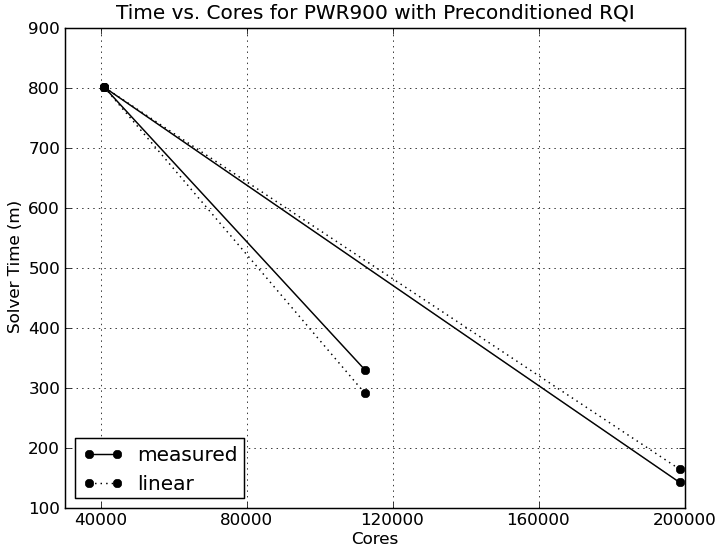
\includegraphics [width=0.8\textwidth, height=0.5\textheight] {PWRPrecondRQI}
   \end{center}
   \caption{PWR900, Strong Scaling with Preconditioned Rayleigh Quotient Iteration}
   \label{fig:PWRprecondRQI}
\end{figure}

The solver time decreased rapidly with increasing cores, and the 198,528-core test performed better than linearly. %The 11 set time was 88\% efficient, and 22 sets had an efficiency of 115\%. 
The high efficiency and the increase in efficiency with sets was expected based on the previous two multiset studies. That the scaling is so good is likely attributable to the multigrid preconditioner. However, this demonstrates that RQI can use multisets without causing the scaling to degrade is some significant way. 

While rigorous timing comparisons cannot be made between preconditioned RQI and unpreconditioned PI, some general remarks can be made. The unpreconditioned PI test of the PWR with 11 sets on 112,200 cores had a solve time of 36.3 minutes. The preconditioned RQI time was 330.38 minutes, or about an order of magnitude longer. This is not a favorable comparison, but it is expected the comparison would improve if 1) the two tests used the same tolerances, 2) the preconditioned case used a reduced preconditioner angle set, 3) the number of energy grid levels were reduced, and 4) the preconditioner were optimized in general.

The PI case was likely solved with an upscattering tolerance of $1 \times 10^{-3}$ rather than $1 \times 10^{-4}$, though this number cannot be confirmed. Converging to the tighter tolerance would likely increase the calculation time for PI. The 4 set preconditioned RQI tests showed that using $S_{2}$ rather than $S_{12}$ reduced solve time by about 75\% while still getting the right answer. Improvement of that order would likely be seen in the 11 set case as well. The number of grids with 11 sets could be reduced from three to two without an iteration count impact and this would reduce preconditioner time. Finally, any optimization of the preconditioner would bring the two solve times closer together. Another possible but not guaranteed way to reduce the preconditioned RQI time is by using a smaller amount of preconditioning, like $w1r2v2$. This might be sufficient to converge RQI and might also decrease calculation time. 

\subsection{Summary of Findings}
All of the test results lead to some useful conclusions. In terms of preconditioning parameters, increasing $r$ and/or $v$ almost always decreased Krylov iteration count and sometimes decreased eigenvalue iteration count. The Krylov iteration reduction is determined by the total number of relaxations, which is determined by $r$ and $v$. All of the relaxations can be executed via $r$ or $v$ or some combination. The way the relaxations are distributed between $r$ and $v$ may influence the calculation time since the distribution changes the number of prolongation and restriction operations. 

It would seem that the order in which the relaxations are done could have an impact on the end iteration count. Smoothing a lot on each grid once could have a different effect on the error modes than smoothing a little bit, going down a grid and smoothing a little, smoothing a little more on the first grid, and then repeating. Different components of the error would be reduced in a different order in a way that could have an impact. If this does have an impact, though, it was not large enough to influence the end iteration count in the tests conducted.  
 
Overall, a moderate amount of preconditioning gave the best performance. A little bit of preconditioning did not do enough to ensure eigenvector convergence in all cases. Using a large number of relaxations and V-cycles to reduce iteration count was often not worth the extra run time. Because the preconditioner is not yet optimized it is difficult to provide strong conclusions about exactly what $r$ and $v$ values are most worthwhile. 
 
Increasing the weight a small amount, up to about 1.3 or 1.4, was generally beneficial. However, using a large weight was sometimes detrimental. Weight was the least consistent parameter, behaving differently in different problems with different degrees of preconditioning. Using a weight of 1 with small $r$ and $v$ and a weight between 1 and 1.3 for an intermediate $r$ and $v$ is probably the safest approach. 

Note that the improvement gained from the multigrid-in-energy preconditioner is non-linear; doubling the preconditioning parameters does not necessarily halve the iteration count. This means the impact of preconditioning parameters can not be accurately predicted ahead of time. The wider computational community's experience with preconditioning Krylov methods is also that performance cannot be well predicted \emph{a priori} in general.

Some lessons were also learned about preconditioner choices besides $w$, $r$, and $v$. GMRES, which is the default Krylov method, should always be selected over BiCGSTAB when using RQI. The shifted operator should never be used inside the preconditioner when there are reflecting boundaries, and should probably never be used at all. While it reduced the number of iterations in the vacuum test case compared to the unshifted operator, it was not robust and gave no indication when it resulted in incorrect answers. The default behavior is to use the unshifted operator. 

Using the reduced angular expansion option within the preconditioner may have a lot of pay off. In the two cases where it was tried it reduced calculation time noticeably. This option must be turned on by the user, and should be exploited when possible. It is applicable when the angular expansion is larger than $S_{2}$, but is currently limited to vacuum boundary cases.

Based on the multiset results, the multigrid method likely does not need to restrict down to one energy group. The depth of the V-cycles should be set to only a few or two levels, and experiments should be done to investigate the effect on serial calculation time and energy scaling. Implementing this choice requires changing the code itself. To give the user more control over this setting the code could be modified to provide a user-input option that controls the depth of the V-cycle.

Overall, the multigrid-in-energy preconditioner was shown to be very effective at reducing iteration count. It was demonstrated that it takes advantage of energy parallelization efficiently. The tests showed that RQI can be used with the new preconditioner to solve problems it could not solve without it. They also showed that preconditioned RQI can be faster than preconditioned PI for challenging problems. Will preconditioned RQI ever be faster than unpreconditioned PI? That cannot be answer based on the existing data, but the data do not exclude that possibility. 

%-------------------------------------------------------------------------------------------------------
\section{Implications}
There were two primary motivations for the multigrid-in-energy preconditioner. Power iteration, the traditional eigenvalue solver, can converge slowly for systems with high dominance ratios. This motivated the implementation of RQI, which uses an optimal shift to converge loosely coupled systems in fewer eigenvalue iterations. As was found in Chapter~\ref{sec:Chp3}, Krylov methods stagnate for poorly conditioned systems such as those created by RQI. Preconditioning is therefore required to be able to use RQI for real problems. 

In addition, ever-expanding computers allow codes to use hundreds of thousands of cores for large computations. Any new preconditioner in Denovo must be able to use these machines efficiently. At its core, the multigroup in energy preconditioner is designed to take advantage of energy parallelization. The way it has been implemented, the multigrid-in-energy method does not require any inter-set communication and it is always energy-load balanced so it should scale extremely well. The new energy decomposition provided by the MG Krylov solver is what allows this preconditioner to be parallelized in energy. Without that, the preconditioner would not be as attractive. 

Using a multigrid method in the energy domain is new for the neutron transport equation. No similar ideas were found in the literature. This is not surprising because the energy scaling motivation for the preconditioner is relatively new as well. Only in the last few years has parallelization in energy become feasible. Without that driver there was no reason to do multigrid in energy. 

The goals for the new preconditioner were to decrease iteration count for at least some problems, to enable RQI, and to be decomposable in energy. All goals were achieved. The multigrid-in-energy preconditioner reduced the number of Krylov iterations for all problem types as long as the eigenvector converged. In some cases it reduced the number of eigenvalue iterations as well. The preconditioner makes the use of RQI in real problems possible, and it scales to hundreds of thousands of cores without trouble. 



\separatorpage{}








          % Chapter 4, ``preconditioning''
 % Thesis, Chapter 5
% by Rachel Slaybaugh

\chapter{Summary}
\label{sec:Chp5}
To enhance and improve the design of nuclear systems, high-fidelity neutron fluxes are required. For today's problems, high-fidelity means thousands $\times$ thousands $\times$ thousands of mesh points, up to $\sim$150 energy groups, accurate scattering expansions, and the use of many directions. Leadership-class machines provide platforms on which problems of this size can be solved in a reasonable amount of time. Computing such fluxes accurately and efficiently requires numerical methods with good convergence properties and algorithms that can scale to hundreds of thousands of cores. 

Many 3-D deterministic transport codes can scale in space and angle to tens of thousands of cores. They typically rely on methods such as Gauss Seidel for fixed source problems and power iteration wrapped around GS for eigenvalue problems. Within group solvers range from source iteration to Krylov methods. In many cases these methods are accelerated with strategies like CMR, TTG, DSA, and others discussed earlier in this document. Nevertheless, these calculations can be slow to converge for challenging systems like those with highly scattering materials or high dominance ratios. 

Three methods have been added to Denovo that are designed to improve convergence and enable the full use of leadership-class computers. The driving concept of this research is to use Rayleigh quotient iteration for solving the $k$-eigenvalue problem in 3-D neutron transport. This objective was not tractable with the tools originally available in Denovo. The multigroup Krylov solver and multigrid-in-energy preconditioner were developed to facilitate RQI, though both of these tools are also useful on their own. This chapter reviews each method, highlights associated results, recommends future work, and closes with some discussion about their potential impact. 

\section{Multigroup Krylov Solver}
Before this work began, Denovo had been shown to exhibit good strong scaling in space and angle to about 20,000 cores using Gauss Seidel as its multigroup solver. The first method added was a multigroup Krylov solver that was designed to improve convergence when compared to Gauss Seidel and to dramatically increase the number cores Denovo can use. 

Instead of sequentially solving each group with some inner iteration method and then using GS for outer iterations to converge the up-scattering, the MG Krylov solver treats a block of groups (either all groups or just upscattering groups) at once such that the inner-outer iteration structure is removed. Using a Krylov method over the upscattering block instead of GS resulted in much faster convergence, both in terms of time and iteration count. No other transport codes were found that apply Krylov solvers over a block of groups without also needing inner iterations. 

In addition, the block Krylov solver allows energy groups to be solved simultaneously because the multigroup-sized matrix vector multiply can be divided up in energy and parallelized. The block is broken into energy sets and each set is handled by a different group of cores. The spatial decomposition does not change, and each set gets the entire spatial mesh such that space-angle scaling remains intact.  Other \Sn transport codes that are parallelized in the energy dimension could not be found. Energy sets extend the number of cores that can be used efficiently by Denovo from tens of thousands to hundreds of thousands. 

Three test problems were used to investigate how the new method compares to GS, and how it scales in energy. The iron graphite cube and PWR900 tests showed MG Krylov to be much faster than GS, even when GS is accelerated. Once the multiset communication was optimized, the strong scaling performance of block Krylov was shown to be nearly perfect to 50,000 cores and reasonable to 200,000 cores. Weak scaling in energy was not as good, though it was not tested with the improved multiset communication strategy. The addition of energy sets enabled Denovo to use 100,000 and 200,000 cores with reasonable efficiency; this would not have been possible for the same problems with KBA alone. 

%Two test problems were used to investigate the new method's functionality, how it compares to GS, and how it scales in energy. The small fixed source, iron graphite cube showed that the Krylov solver was much faster than unaccelerated GS. The use of graphite made this problem particularly challenging for GS. A full PWR was also studied with power iteration as the eigenvalue solver. The 2-group versions of this problem showed the MG Krylov solver to be much faster than accelerated GS. Both tests confirmed that the new multigroup Krylov solver has the potential to substantially outperform Gauss Seidel in challenging cases and problems of interest.  

%The effect of using energy sets was also investigated with both test problems. The iron graphite cube verified that the new MG solver works successfully with multisets. The large PWR problem that had over 1.7 trillion degrees of freedom was used to investigate strong scaling. Three cases that used different combinations of $\sim$100,000 or $\sim$200,000 cores, and 11 or 22 energy sets were computed on Jaguar. This is exactly the type and scale of calculation the MG Krylov solver was made to handle.

%The strong scaling study gave mixed results. Initially, doubling the energy sets with approximately the same spatial decomposition yielded 80\% efficient scaling. Doubling the spatial blocks with the energy sets held constant gave 86\% efficient scaling. Both of those numbers are great. However, some communication was optimized in Denovo and the energy scaling cases were repeated. This reduced the efficiency to only 62\%. Some improvement in the multiset communication has been implemented since these results were found, but the tests have not been repeated to see the effect on energy scaling. 

%The PWR problem was also used for a weak scaling study. The ratio of calculated time to ideal time was 1.019 when the problem was expanded from 17,424 cores to 112,200 cores. The weak scaling performance was very good. 

A multigroup Krylov solver has not been previously pursued because of computer architecture limitations in the past. It is only now that there are machines with memories large enough to accommodate such large Krylov subspaces and that have enough cores to warrant the capability of using hundreds of thousands of cores. Denovo has been used successfully on a machine of this size for a real problem because of the new energy decomposition. The test problems demonstrated that the new method accomplishes the goal of accelerating transport calculations by fully using new computers.

\section{Rayleigh Quotient Iteration}
Finding the criticality state of a multiplying nuclear system is one of the most important kinds of analysis done for nuclear systems. The standard eigenvalue solution methods can converge slowly in some important instances. To design new reactors, a better eigenvalue solver is needed. One of a class of methods that solves a modified system with identical eigenvectors and shifted eigenvalues, Rayleigh quotient iteration finds the dominant eigenvalue using a mathematically optimal shift. Theory indicates that RQI should converge in fewer iterations than traditional eigenvalue solvers.

The addition of RQI, though, would not be possible without the MG Krylov solver. Within Denovo, the Rayleigh quotient in RQI multiplies the fission matrix which is then subtracted from the scattering matrix. This results in a set of equations that is mathematically equivalent to having up-scattering in every group, so the scattering matrix becomes energy-block dense. Handling energy-block dense systems when there are more than a few energy groups is not tractable with GS as the multigroup solver. It is only the MG Krylov solver that makes RQI a reasonable idea when there are many energy groups.

%In return, RQI takes fuller advantage of the energy parallelization made available by the block Krylov solver than power iteration or fixed source solves can. Every group can be solved simultaneously since every group looks like it has upscattering. In the upper limit, there can be as many energy sets as groups in a problem. This degree of energy parallelization only makes sense with RQI. 

There is, however, a drawback that comes from using RQI with a Krylov method. When the Rayleigh quotient is close to the eigenvalue being sought, the system becomes ill-conditioned. The closer RQI comes to solving the problem, the worse the conditioning becomes. Krylov methods can converge very slowly and may not be backwards stable for ill-conditioned systems. If the multigroup iterations do not converge the eigenvector inside the RQI calculations, then RQI itself will not converge as it will not be able to find an accurate RQ.

Three sizes of problems, small, medium, and large, were used to test whether RQI requires fewer iterations than power iteration and whether the shift prevents the Krylov solver from converging. The small problems showed RQI could correctly find the eigenvalue and eigenvector in fewer iterations than power iteration. RQI began to falter with the medium problem, finding an eigenvalue only close to the reference and failing to converge the eigenvalue or vector. With the large problems RQI did not work at all.

%Two small problems, one with reflecting and one with vacuum boundaries, demonstrated that RQI could correctly find the eigenvalue and eigenvector in fewer iterations than power iteration. 

%The intermediately sized problem with reflecting boundary conditions did not work as well. The Krylov solver was not able to converge the flux moments in a reasonable number of iterations. Then the eigenvalue part of the calculation did not converge because there was not an accurate eigenvector from which to make the eigenvalue guess. This problem seemed to have an eigenvector guess that was close to correct, though, because the RQI-computed eigenvalue only differed from the reference $k$ by 0.0033. With two benchmark reactor problems, RQI did not work at all. The multigroup iterations did not converge and the eigenvalue was not close to the reference. 

Valuable insights were gained from the RQI test results despite the failures. Simple problems demonstrated that RQI can find correct solutions and converge in fewer iterations than power iteration, thus it has promise for accelerating eigenvalue calculations. The failures showed that for real problems the matrix system becomes too ill-conditioned to work with a Krylov solver. If preconditioning can get the Krylov multigroup solves to converge, then RQI will likely be a successful method that can solve at least some challenging problems in fewer eigenvalue and total Krylov iterations than power iteration. 

Despite the clear theoretical edge RQI has over many other iterative eigenvalue methods, it has never been used for 3-D neutron transport before, largely because of the application of the shift. Traditional multigroup solvers like Gauss Seidel cannot treat energy-block-dense scattering systems efficiently. The MG Krylov solver lets RQI be used in this context, and enables the parallelization of eigenvalue calculations to hundreds of thousands of cores. 

\section{Multigrid in Energy}
Another way to reduce calculation time is by reducing the number of iterations needed for convergence through preconditioning. %If the savings from a lower iteration count is more than the cost of the extra work done in making and applying the preconditioner, the result is a faster code. 
A multigrid-in-energy preconditioner was added to Denovo to reduce iteration count for all problem types, and to address the convergence issues arising from RQI. 

Iterative methods reduce oscillatory error effectively, but not smoother error. The smooth error can prevent iterative methods from converging. This behavior is characterized by rapid error reduction in the first several iterations followed by very little error reduction. Such a trend was observed when RQI failed. Multigrid methods selectively remove smoother error components and are therefore ideal for accelerating this type of problem. Thus, a multigrid preconditioner should work very well with RQI. 

The  preconditioner conducts a multigrid method in the energy dimension. A set of energy grids with increasingly coarse energy group structures are created. To apply the preconditioner, the residual is restricted and prolonged between these grids and weighted Richardson iteration is done on each grid to remove different error modes. The V-cycle(s) result in a vector that corrects the current flux estimate. 

%Restricting a problem from a fine energy grid to a coarser energy grid makes the error modes that appeared smooth on the fine grid become oscillatory. An iterative scheme can be applied on the coarse grid to reduce the error components that appear oscillatory there. The problem can then be prolonged back to the fine energy grid where the troublesome error modes have now been removed. 

The multigrid preconditioner is implemented in a way that easily and efficiently takes advantage of the new energy decomposition. The multigrid algorithm is applied within each energy set such that the energy groups are only restricted and prolonged between groups on that set. Sets do not have to communicate with one another in the preconditioner, and using more sets creates fewer total grid levels. An alternative strategy that was not investigated is to restrict groups across sets such that the total number of grid levels is set-count independent. 

Many tests were done to investigate the behavior of the new preconditioner. All of the tests showed that the preconditioner can be useful for many problem types: reflecting and vacuum boundaries, few and many groups, fixed source and eigenvalue. The preconditioner always worked well for fixed source problems. Multigrid in energy also dramatically reduced iteration count in all tests with power iteration. 

The preconditioning did not always work well for problems that RQI could already solve, though these were easy problems that did not need to be preconditioned. More importantly, though, problems that RQI could not solve without preconditioning did converge with it. As problems became more realistic, RQI benefited more from preconditioning. Preconditioned RQI used fewer iterations and was substantially faster than preconditioned power iteration for the full-facility PWR.

There was one test RQI did not handle well. It highlighted that RQI is a somewhat brittle method that does not always work because of the ill-conditioning issue. When it does work, it works very well. As a general rule, the output of RQI should not be trusted if the Krylov iterations do not converge on every iteration, even if $k$ does converge. $k$ should only be considered valid when all of the multigroup iterations converge. To help ensure the eigenvector is converged for real problems, a moderate amount of preconditioning (e.g., $w1r3v3$) should be used. 

%The preconditioner always worked well for fixed source problems. The number of iterations were reduced for the vacuum and reflecting unit tests as well as for the iron and graphite cube problem. Multigrid in energy also always worked well with power iteration, dramatically reducing iteration count in all tests. 

%For tough fixed source and eigenvalue problems solved with PI, the preconditioner could prove to be very beneficial once it has been optimized. The timing comparisons were not favorable, but there are a several suggestions in the future work section that could remedy this.

%With RQI, the preconditioning did not always work well for problems that RQI could already solve, though these were easy problems that did not need to be preconditioned. In these simple cases preconditioned power iteration worked better than preconditioned RQI. All of the tests where this was the case had low dominance ratios. The spectral properties of these systems are good for PI and are not necessarily as good for RQI.

%Problems that RQI could not solve without preconditioning did converge with it. As problems became more realistic, RQI benefited more from preconditioning. For the 2-D benchmark problem, RQI worked well and was slightly inferior to preconditioned PI. In the 3-D benchmark study RQI performed better than PI for intermediate and large amounts of preconditioning. RQI was substantially better than PI in the full-facility PWR test case.

%The one trouble case was the intermediate infinite medium problem. RQI always had difficultly and preconditioning did not help much. It is unclear why this happened. It seemed that RQI did not perform as well for any problem that had six reflecting boundaries, though this was the only such case where RQI was unreliable. Power iteration, however, solved the problem without issue. 

%This test highlights that RQI is a somewhat brittle method. It does not always work because of the ill-conditioning issue. When it does work, it works very well. As a general rule, the output of RQI should not be trusted if the Krylov iterations do not converge on every iteration, even if $k$ does converge. In the cases where this happened the $k$ was usually correct, but it was not always correct. $k$ should only be considered valid when all of the multigroup iterations converge. To help ensure the eigenvector is converged for real problems, a moderate amount of preconditioning (e.g., $w1r3v3$) should be used. 

The multigrid method worked efficiently with multisets and scaled very well. %This is likely for two reasons. One is that the preconditioner did not add inter-set communication, so changing the number of sets does not increase the cost of the preconditioner from a communication standpoint. The second is that the reduction in number of grids makes the preconditioner less expensive with increasing set count. 
%
Not only were there no negative impacts from using more energy sets in the preconditioner, but scaling was actually improved by its use. The energy scaling performance with this implementation of the multigrid-in-energy method suggests that this parallelization strategy is better than the one that communicates across sets. 

A multigrid method has never been applied to the energy portion of phase space for the neutron transport problem before. This is not surprising because the motivation for the preconditioner is relatively new as well. Only in the last few years have energy parallelization and Rayleigh quotient iteration become feasible. Without those drivers there was no reason to do multigrid in energy.

\section{Suggested Future Work}
While many interesting things about these three methods have been found, there are still many questions to be answered. There are also a few remaining implementation details that will make these methods more flexible. This section suggests some ideas for further investigation that would help answer some questions more decisively, could guide how and when these methods should be used, and could lead to their improvement. Some suggestions are research-based, some require implementation, and some are simply tests.

\subsection{Testing}
Most of the problems where direct comparison between PI and RQI was possible did not have characteristics that represented the kinds of problems that scientists want to solve in practice. The cases that did have realistic characteristics could not be meaningfully compared. Tests that conclusively show whether or not preconditioned RQI can be better than unpreconditioned PI are of highest priority.

Calculations with the PWR900 should be done for this purpose, all using the same spatial decomposition, the same number of energy sets, and the same tolerances. The preconditioned RQI calculations should use $S_{2}$ in the preconditioner, only two grids in energy, and a few different preconditioning parameters sets. These results should be compared to unpreconditioned PI. In addition, at least one PI calculation with the same preconditioning options as RQI should be run to completion so a full comparison can be made. 

One or two other test problems with parameter consistency across calculations and with realistic properties, such as high dominance ratios, are also needed. Doing sound comparisons between a few different problems should provide enough information to make conclusions about the relative benefit of RQI when compared to PI.

More investigation into weak scaling for all solvers is needed as well. The performance with MG Krylov reported in Chapter~\ref{sec:Chp2} was very poor. Such a study should be repeated with the optimized multiset communication. If the results are not improved, a deeper investigation into the causes and possible remedies is warranted. 

No weak scaling studies have been done for the preconditioner or RQI. Once the MG Krylov study has been completed, a preconditioned fixed source weak scaling study should be done. The performance with the preconditioner can be compared to the performance with MG Krylov alone. After that, a preconditioned RQI weak scaling study can be done, informed by the MG Krylov and preconditioned fixed source results.

\subsection{Optimization}
RQI and multigrid in energy can both by improvement through implementation changes. \\Rayleigh quotient iteration can not be used with energy sets when there are reflecting boundaries. This capability should be added as it vastly expands the number of problems for which it is applicable. This also expands the suite of tests available to study energy scaling with RQI. For example, the 2-D and 3-D c5g7 benchmark problems would then be available for these kinds of tests. 

Using a reduced number of solution directions inside the preconditioner is also not available when there are reflecting boundaries. This option seems like it may be very useful for reducing the time taken by the preconditioner. Ensuring all problems have this tool available will increase the benefit of preconditioning for problems using anything besides $S_{2}$.

Related to this, the benefit gained by using the smaller angle set in the preconditioner should be quantified. If it is found that the benefit is large and there is little or no impact on iteration reduction, then the default behavior could be changed to always use $S_{2}$, or $S_{N/2}$, etc.\ in the preconditioner with an input option to specify something else if desired. 

A crucial area of work is optimizing the preconditioner to make it faster. The multiset tests indicate that reducing the total number of energy grids to two or three regardless of the number of energy groups will not impact the iteration reduction gained from preconditioning. This change alone would greatly reduce the time the preconditioner takes for problems with more than a few energy groups. A few different grid depths should be investigated to assess what is best. Much speed can probably be gained by more efficient C++ coding as well. 

Once ideal V-cycle depth has been determined, guidance has been developed about using reduced angle sets, and any C++-related optimization has been added, comparison studies should be considered for time. The tests done in this work can be repeated or similar studies using problems with practical engineering properties can be done for this purpose. Energy scaling studies will also be needed to learn how the preconditioner scales with a different implementation of the number of grid levels.  

\subsection{Research}
A more research-oriented line of investigation is to try different ways to test for convergence within RQI. Right now the current Rayleigh quotient is compared to the previous one. A different criterion might be better or lead to more accuracy, for example using the eigenvector instead of the eigenvalue. There has also been some convergence analysis for RQI and research discussing interesting ways to set RQI convergence criteria that would inform this research. See for example Notay \cite{Notay2003} and Szyld \cite{Szyld2011}.
    
Changing some of the solution details inside the preconditioner is another avenue of research. Relaxation methods besides weighted Richardson should be considered. It may be that something like Jacobi, or successive over relaxation, or another iterative method would work better. The behavior of the weight parameter inside the preconditioner was difficult to characterize in a generic way and occasionally caused poor behavior. Weight is the only parameter that is specifically related to Richardson. Another method would avoid that difficulty and could be more robust as a result. The preconditioner might also benefit from different prolongation and/or restriction operators. A few different methods should be tried and tested to see if any impact is made. 

Some of these suggestions require more time and effort than others. A shallower default V-cycle will be easy to implement. Adding reduced angle sets and RQI with multisets for reflecting boundaries may be more work, but will be important to have. Using a different RQI convergence strategy or a different relaxation method are topics that likely require mathematical analysis and more in depth research. Most importantly, though, more testing should be done to more rigorously understand the new methods and their impacts in different scenarios.  

\section{Closing Remarks}
The goal of this research was to accelerate transport calculations with methods that can take full advantage of modern leadership-class comuputers, facilitating the design of better nuclear systems. Three complimentary methods were implemented that accomplish this goal to varying degrees. 

At the outset of this work, Denovo could be decomposed in five of the six dimensions of phase space over which the steady-state transport equation is solved in a way that restricted it to about 20,000 cores for a problem with 500 million cells. The original suite of solvers included Gauss Seidel as the multigroup solver and power iteration wrapped around GS as the eigenvalue solver. These solvers have some significant limitations in many cases of interest. 

The new multigroup Krylov solver converges more quickly than GS and enables energy decomposition such that Denovo can scale to hundreds of thousands of cores. The new multigrid-in-energy preconditioner reduces iteration count for many problem types and takes advantage of the new energy decomposition such that it can scale very efficiently. These two tools are useful on their own, but together they allow the Rayleigh quotient iteration eigenvalue solver to work.

The real motivation of this work was to add RQI, which should converge in fewer iterations that power iteration for large and challenging problems. RQI creates shifted systems that would not be tractable without the MG Krylov solver. It also creates ill-conditioned matrices that cannot converge without the multigrid-in-energy preconditioner. Using these methods, RQI converged in fewer iterations and in less time than preconditioned PI for a full-facility PWR on 200,000 cores. 

The methods added in this research accelerated Denovo in multiple ways. This acceleration helps enable the solution of today's ``grand challenge'' problems. It is hoped that improved methods will lead to improved reactor designs and systems, and that the frontier of computational challenges will be moved forward.  


         % Chapter 5, ``comclusions'

\bibliography{Thesis}         % Make the bibliography

\begin{appendices}       % Start of the Appendix Chapters.  
                                          % If there is only one Appendix Chapter, then use \begin{appendix}
% Prelim, Appendix A
% by Rachel Slaybaugh

\chapter{Diffusion Equation}
\label{sec:AppendixA}
The diffusion approximation is a widely used simplification that reduces the computational complexity of the transport equation. The approximation is that the angular dependence of the flux is unimportant, so the direction component of the transport equation can be discarded. Physically this means that neutrons move against their concentration gradient like just heat diffuses through a conductor. The information in this section is derived from Duderstadt and Hamilton's \emph{Nuclear Reactor Analysis} \cite{Duderstadt1976} and neglects fission for simplicity. 

The first step in applying this approximation is to integrate the angular dependence out of Equation \eqref{eq:neutron transport}, resulting in the neutron continuity equation:
%
\begin{equation}
  \nabla \cdot J(\vec{r},E) + \Macro(\vec{r},E)\phi(\vec{r},E) = \int \:dE' \:\Macro_{s}(\vec{r}, E' \to E)\phi(\vec{r},E') + Q_{ex}(\vec{r},E) \:,
  \label{eq:continuity} 
\end{equation}
%
where the following definitions have been used:\\
\indent $J(\vec{r},E) = \int d\vOmega \:\vOmega \psi(\vec{r}, \vOmega, E)$ is the neutron current \\
\indent  $\phi(\vec{r},E) = \int d\vOmega \:\psi(\vec{r}, \vOmega, E)$ is the scalar flux, and \\
\indent $Q_{ex} (\vec{r},E)= \int d\vOmega \:q_{ex}(\vec{r}, \vOmega, E)$ is the external source.

Unfortunately, this simplifying approximation added another unknown, $J$, which leaves one equation with two unknowns. In an attempt to eliminate one of these unknowns, Equation \eqref{eq:continuity} is multiplied by $\hat{\Omega}$ and integrated over angle again to obtain the first angular moment:
%
\begin{align}
  \nabla \cdot \int  d\vOmega \:\vOmega \vOmega \psi(\vec{r}, \vOmega, E) &+ \Macro(\vec{r},E) J(\vec{r},E)= \nonumber \\
  &\int dE' \:\Macro_{s1}(\vec{r}, E' \to E)J(\vec{r},E') + \int d\vOmega \int d\vOmega \:\vOmega q_{ex} \:,
  \label{eq:current1}
\end{align}
%
where $\Macro_{s1}  = \int d\vOmega \:\vOmega \Macro_{s}$. The first angular moment form of the equation cannot be solved either because the streaming (first) term is still unknown. 

To make Equation \eqref{eq:current1} solvable, the original assumption is modified to assert that the angular flux is weakly, in fact linearly, dependent on angle rather than independent of angle. To implement this assumption the angular flux is expanded in angle and only the first two terms are retained:  
%
\begin{equation}
  \psi(\vec{r}, \vOmega, E) \cong \frac{1}{4 \pi} \phi(\vec{r}, E) + \frac{3}{4 \pi}J(\vec{r}, E) \cdot \vOmega \:.
  \label{eq:angExpand} 
\end{equation}
The truncated angular flux is then inserted into the streaming term in Equation \eqref{eq:current1}, giving 
%
\begin{equation}
  \nabla \cdot \int d \vOmega \:\vOmega \vOmega \psi(\vec{r}, \vOmega, E)  \cong \frac{1}{3} \nabla \phi(\vec{r}, E) \:. 
  \label{eq:firstTerm}
\end{equation}

Next, the scattering source term is simplified in angle and energy. To address the angular dependence define $\bar{\mu}_{0}$ as the average cosine of the scattering angle, which, temporarily suppressing energy, gives $\Macro_{s1} = \bar{\mu}_{0}\Macro_{s}$. For elastic scattering from stationary nuclei when s-wave scattering is present in the center of mass frame, $\bar{\mu_{0}} = \frac{2}{3A}$ where $A$ is atomic mass number. A common procedure to simplify the energy dependence is to neglect the anisotropic contribution to energy transfer in a scattering collision. Mathematically this means $\Macro_{s1}(E' \to E) = \Macro_{s1}(E) \delta(E' = E)$, giving $\int dE' \:\Macro_{s1}(\vec{r}, E' \to E)J(\vec{r},E') = \bar{\mu_{0}}\Macro_{s}(\vec{r},E)J(\vec{r},E)$. Finally, it is assumed that the external source is isotropic, $\int  d\vOmega \int d\vOmega \:\vOmega q_{ex} = 0$.

If these approximations are all included and Equation \eqref{eq:current1} is solved for $J$, the result is Fick's Law:
%
\begin{equation}
  J(\vec{r},E) \cong -\frac{1}{3(\Macro(\vec{r},E) - \bar{\mu_{0}}\Macro_{s}(\vec{r},E))} \nabla \phi (\vec{r},E) = -D(\vec{r},E) \nabla \phi (\vec{r},E) \:.
\end{equation}
%
Fick's Law can be introduced back into Equation \eqref{eq:continuity} to obtain the diffusion equation:
%
\begin{equation}
  -\nabla \cdot D(\vec{r},E) \nabla \phi(\vec{r},E) + \Macro(\vec{r},E)\phi(\vec{r},E) = \int dE' \:\Macro_{s}(\vec{r}, E' \to E)\phi(\vec{r},E') + q_{ex}(\vec{r},E) \:.
  \label{eq:diffusion}
\end{equation}

This equation now includes several assumptions which are valid when the solution is not near a void, boundary, source, or strong absorber. While these requirements can be quite restrictive, the diffusion equation has been used frequently for analysis of nuclear systems throughout the history of the nuclear industry.

Some terms from this section that are used when describing DSA in Chapter \ref{sec:Chp4} are:
\begin{align}
  \Macro_{tr} &= \Macro(\vec{r},E) - \bar{\mu_{0}}\Macro_{s}(\vec{r},E) \qquad \text{is the transport cross section, and}\\
  \ve{C} &= -\nabla \cdot \frac{1}{3\Macro_{tr}}\nabla+ \Macro(\vec{r},E) \qquad \text{is the diffusion operator.}
\end{align}

			 
% Prelim, Appendix B
% by Rachel Slaybaugh

\chapter{Krylov Methods}
\label{sec:AppendixB}
This appendix is intended to provide the mathematical details of Krylov methods, including information about restarting Arnoldi and GMRES. While understanding this is not crucial to the developed methods, it is beneficial to be aware of how the underlying solvers work. 

\section{Arnoldi Method}
A general issue with Krylov subspaces is that the columns of $\mathcal{K}_{k}(\ve{A},v_{1})$ become increasingly linearly dependent with increasing $k$. Trying to build solutions out of linear combinations of nearly linearly dependent vectors can fail. The columns of the subspace can be orthogonalized to solve this problem. However, direct orthogonalization will cause some information contained in the subspace to be lost, making more sophisticated factorization methods useful \cite{Stewart2001}. 

In general there are two factorization methods upon which many Krylov methods are based. Some use the Arnoldi method, which generates an orthonormal basis for the Krylov subspace for non-normal matrices, and others use the Lanczos method which creates non-orthogonal bases for normal matrices \cite{Knoll2004}, \cite{Stewart2001}. Denovo has the option of using either restarted GMRES or BiCGSTAB, both of which use the Arnoldi method \cite{Evans2009}.  The remainder of this section will be devoted to developing an understanding of the Arnoldi method.

Fundamentally, Krylov methods are Galerkin or Galerkin-Petrov methods on a Krylov subspace. Galerkin's method uses a few fundamental concepts. One is that an inner product of two functions is zero when the functions are orthogonal: $<f(x), g(x)> = 0$ if $f(x)$ and $g(x)$ are orthogonal. Another is that any function $f(x)$ in a subspace $\mathcal{V}$ can be written as a linear combination of the vectors that make a basis for that function space. Let $\ve{V} = \{\phi_{i}(x) \}_{i=0}^{\infty}$ be the basis for $\mathcal{V}$; if $f(x) \in \mathcal{V}$ then $f(x) = \sum_{j=0}^{\infty} c_{j} \phi_{j}(x)$ for some scalar coefficients $c_{j}$ \cite{Matthews2005}.  

A weighted residual method is a solution technique for solving some linear problem $\ve{A}u = b$ where $u = u_0 + \sum_{i=1}^{n} c_i \phi_i(x)$ is the approximate solution and $u_{0}$ is an initial guess. The solution is found by taking the inner product of some arbitrary weight function, $w(x)$, and the residual, $r(x) = b - \ve{A}u$, $r(x) \in \mathcal{V}$, such that $<w(x), r(x)> = 0$. The solution is the $u$ satisfying this requirement. Galerkin's method is a weighted residual method where the weight function is chosen from the basis functions: $w(x)$ is selected from $\ve{V}$ \cite{Matthews2005}. In the Galerkin-Petrov method, the weight functions come from a subspace other than $\mathcal{V}$, that is $w(x) \in \mathcal{W}$ \cite{Skeel2006}. 

The weighted residual method can also be thought of as a process to minimize the residual. There are a few ways to express this idea. If $\hat{u}$ is the exact minimizer of $r(x) = b - \ve{A}\hat{u}$, then let $u' = \hat{u} + w(x)$ be a close approximation to $\hat{u}$ with $w(x) \in \mathcal{V}$. The residual is minimized if and only if $<w(x), r(x)> = 0$ for all $w(x) \in \mathcal{V}$, meeting the Galerkin condition just described. 

This can also be written as: 
%
\begin{align}
  \text{find } \qquad u \in u_{0} + \mathcal{V} \qquad \text{such that} \qquad r(x) \perp \mathcal{V} \:.
  \label{eq:galerkinMin}
\end{align}
%
Further, if $y$ is the solution to
\begin{equation}
  \ve{V}^{T}\ve{AV}y = \ve{V}^{T} r_{0} \:, \qquad \text{then} \qquad \hat{u} = u_{0} + \ve{V}y \:.
  \label{eq:minResidual}
\end{equation}
This $\hat{u}$ minimizes the residual in the some measure of interest, where the measure is determined by the selection of $y$. In the Petrov-Galerkin formulation, $\ve{W}$ is a basis for subspace $\mathcal{W}$ and the idea is to find $ u \in u_{0} + \mathcal{V}$ such that $r(x) \perp \mathcal{W}$. Now $\ve{V}^T\ve{AW}y = \ve{V}^T r_0$ \cite{Skeel2006}.

Sorensen~\cite{Sorensen1996} and Stewart~\cite{Stewart 2001} use the Galerkin Method in combination with Ritz pairs to understand the Arnoldi method, and this viewpoint will be developed here. To maintain consistency with the main portion of this work, the subspace from which solutions are derived in the next paragraphs will be the Krylov subspace $\mathcal{K}_{k}(\ve{A},v_{1})$, and the equation will be switched to $\ve{A}x = b$.

A vector $z \in \mathcal{K}_{k}(\ve{A},v_{1})$ is defined as a Ritz vector with corresponding Ritz value, $\theta$, if it satisfies the Galerkin condition $<w, \ve{A}z - \theta z> = 0 $ for all $w \in \mathcal{K}_{k}(\ve{A}, v_{1})$. To see why Ritz pairs can be important, define $\hat{p}(\ve{A})$ to be the minimum characteristic polynomial of $\ve{A}$ such that $||\hat{p}(\ve{A})v_{1}|| \le ||q(\ve{A})v_{1}||$ for all monic polynomials $q \ne \hat{p}$ of degree $k$. If $(\theta, z)$ is a Ritz pair for $\ve{A}$, then $\ve{A}z - z\theta = \gamma \hat{p}(\ve{A})v_{1} = g$ for some scalar $\gamma$. When $g = 0$, then the Ritz pair is an eigenpair. When $g$ is small, the Ritz pair is likely a close approximation to an eigenpair of $\ve{A}$ \cite{Sorensen1996}. 

These ideas can be assembled to understand why the Arnoldi method works. Let $\ve{V}$ be a basis for a Krylov subspace $\mathcal{K}_{k}(\ve{A},v_{1})$, and $\mathcal{X} \in \mathcal{K}_{k}(\ve{A},v_{1})$ be an eigenspace of $\ve{A}$. When solving $\ve{A}x = b$, the subspace $\mathcal{K}_{k}(\ve{A},v_{1})$ and the vector $x$ must satisfy
\begin{enumerate}
  \item $x \in \mathcal{K}_{k}(\ve{A},v_{1})$ and
  \item $r = \ve{A}x - b \perp \mathcal{K}_{k}(\ve{A},v_{1})$. 
\end{enumerate} 
%
Let $\ve{H} = \ve{V}^{T}\ve{AV}$. There is an eigenpair $(\theta, x)$ of $\ve{H}$ such that $(\theta, \ve{V}x)$ is an eigenpair of $\ve{A}$. To reduce notational clutter let $z = \ve{V}x$, giving $\ve{A}z = \theta z$ \cite{Stewart2001}. 

If $\ve{V}$ is an orthonormal basis for  $\mathcal{K}_{k}(A,v_{1})$, then $(\theta, z)$ is a Ritz pair if and only if $x = \ve{V}y$ with $\ve{H}y = \theta y$ for some $y$. Noting the definition of $\ve{H}$, comparing to Equation \eqref{eq:minResidual}, and doing some basic matrix manipulation, it can be seen that this $y$ minimizes the residual. As the residual tends toward zero, the Ritz pair converges to an approximate eigenpair of $\ve{A}$ \cite{Stewart2001}. Another way to state this is to revisit the polynomial identity expressing the minimum residual. It can be shown that $\ve{AV}y - \ve{VH}y = \gamma \hat{p}(\ve{A})v_{1} = g$. As $g \to 0$, the Ritz pair approaches the eigenpair of $\ve{A}$ \cite{Sorensen1996}. 

In summary, the eigenpairs of $\ve{A}$ are approximated by the eigenpairs of $\ve{H}$. These eigenvalues and/or eigenvectors are subsequently used in different ways by different Krylov methods to formulate the solution to $\ve{A}x = b$ to achieve specific goals, like minimizing the residual in a certain norm. The Galerkin condition is used to ensure the eigenpairs of $\ve{H}$ become increasingly good approximations to those of $\ve{A}$ as the size of the Krylov subspace increases. 

The Arnoldi method is a process of establishing the $\ve{V}$ and $\ve{H}$ discussed above \cite{Stewart2001}. $\ve{H}$ is an orthogonal projection of $\ve{A}$ onto the basis $\ve{V}$ and is upper Hessenberg in form. The Gram-Schmidt method (or the modified Gram-Schmidt method) computes $\ve{V}$. The Arnoldi method generates a Ritz estimate for the Ritz pair at each iteration. Using these terms and ideas, the Arnoldi algorithm shown in Algorithm~\ref{algo:Arnoldi} can be understood \cite{Saad1986}, \cite{Sorensen1996}.
%
\begin{algorithm}
  \caption{ Orthogonal Arnoldi Method}
  $r_0 = b - \ve{A}x_0$ \\
  $v_1 = \frac{r_0}{||r_0||}$ \\
  For $j = 1$ to $k$: 
  \begin{list}{}{\hspace{2em}}
    \item $h_{i,j} = v_i \ve{A} v_j$, $i = 1, \dots, j$ 
    \item $\text{ } \hat{v}_{j+1} = \ve{A}v_j - \sum_{i=1}^{j} v_j h_{i,j}$ 
    \item $\text{ } h_{j+1,j} = ||\hat{v}_{j+1}||$ 
    \item $\text{ } v_{j+1} = \frac{\hat{v}_{j+1}} {h_{j+1,j}}$ 
  \end{list}
  Form the solution $x_k = x_0 + \ve{V}_k y_k$, where $y_k = \ve{H}_k^{-1} ||r_0|| e_1$
  \label{algo:Arnoldi}
\end{algorithm}

The $k$th step of an Arnoldi factorization can be written as: 
%
\begin{equation}
  \ve{AV}_{k} = \ve{V}_{k}\ve{H}_{k} + g_{k}e_{k}^{T} \:,
\end{equation} 
%
where $e_{k}$ is the $k^{th}$ column of the identity matrix and $g$ is the residual. An alternative way to derive the Arnoldi method is as a truncation of the reduction of $\ve{A}$ to Hessenberg form using shifted QR-iteration \cite{Sorensen1996}.

\section{Restarting Arnoldi}
As mentioned above, Krylov methods can become untenable if the subspace is allowed to become large. Restart methods have been developed to handle this. After $m$ iterations the Arnoldi process is halted and a new starting vector, $\hat{v}_1$, is constructed from information gained during the previous $m$ iterations. This new vector is used as the starting vector for another round of the Arnoldi process, which is now using the subspace $\mathcal{K}_k(\ve{A},\hat{v}_1)$ rather than $\mathcal{K}_m(\ve{A},v_1)$. This process is repeated, finding new a starting vector every time the subspace reaches dimension $m$, until convergence. It is assumed that of the $m$ eigenvalues available, only $r$ of them are wanted. Two such restart methods, explicit and implicit, will be discussed here from the viewpoint of how they work and how they preserve the information of interest. 

Explicit restarting applies a polynomial to the starting vector that is designed to damp unwanted components of the eigenvector expansion. There are a few different forms of explicit restarting, but the basic idea begins with splitting the Ritz values into a wanted set, $\Omega_w$, and an unwanted set, $\Omega_u$. In one form of explicit restarting, a combination of wanted eigenvalues are used and in another form a combination of unwanted eigenvectors are used. In both formulations a filter polynomial is used to create a $\hat{v}_1$ that minimizes the residual by removing the unwanted information. The components of the new starting vector therefore become more aligned toward the directions of interest. Unfortunately, filter polynomials are expensive to apply directly and this motivates the need for a more sophisticated restart method \cite{Sorensen1996}, \cite{Stewart2001}.

Implicit restarting is designed to be less expensive than explicit restarting. It uses an implicitly shifted QR mechanism to compress the factorization while retaining information of interest. The idea is to go from a factorization of length $m = p + r$ to one of length $r$ by applying $p$ shifts implicitly. For $j = 1,2,\dots,p$, a QR factorization is done with shifts $\mu_j$ where the shifts are derived from the spectrum of $\ve{H}$, $\sigma(\ve{H}) \equiv \{\lambda \in \mathbb{R}: rank(\ve{H} - \lambda \ve{I}) < n\}$. This gives an $r$-step Arnoldi factorization of the form $\ve{AV}_r \ve{Q} = (\ve{V}_r \ve{Q})(\ve{Q}^T \ve{H}_r \ve{Q}) + g_k e^T_k$. $\ve{Q} = \ve{Q}_1 \ve{Q}_2 \dots \ve{Q}_p$, where $\ve{Q}_j$ is an orthogonal matrix corresponding to shift $\mu_j$, and $g_r = (\ve{V}_r \ve{Q}) e_{r+1} \beta_r + g_m \sigma(\ve{H})$ \cite{Sorensen1996}.

The shift selection strategy can be designed to create a minimal $\hat{v}_1$. The shifted QR factorization reduces the subspace size while eliminating the undesired components. In essence this is implicitly applying a filter polynomial while avoiding the matrix-vector multiplications that would be required in an explicit method. Further, $\mathcal{K}_p(\ve{A},v_1) \subset \mathcal{K}_m(\ve{A}, \hat{v}_1)$, which means the wanted Ritz vectors are still represented in the updated subspace. The implicit method is more efficient and more numerically stable than the explicit restart method \cite{Sorensen1996}, \cite{Stewart2001}.

\section{GMRES}
One of the more popular Krylov methods, which uses the Arnoldi process, is the GMRES algorithm developed by Saad and Schultz~\cite{Saad1986}, \cite{Knoll2004}. Recall that $\ve{V}_{k}$ is an orthonormal basis for the Krylov subspace $\mathcal{K}_{k}(\ve{A}, v_1)$ and that $\ve{H}_{k}$ is the representation of the part of $\ve{A}$ that is in this Krylov subspace formed from the basis $\ve{V}_{k}$. The notation $\bar{\ve{H}}^{k}$ is the $(k+1) \times k$ upper Hessenberg matrix that includes the newest $h_{k+1,k}$ element generated in the Arnolodi process. This satisfies $\ve{AV}_{k} = \ve{V}_{k+1}\bar{\ve{H}}_{k}$ \cite{Saad1986}. 

The distinguishing factor for different Krylov methods is the way in which they select the $y_k$ that makes the solution $x_k = x_0 + \ve{V}_k y_k$. GMRES uses the least squares procedure to find the $y_k$ that minimizes the norm of the residual over $z$ in $\mathcal{K}_{k}(\ve{A}, v_1)$. To accomplish this, the least squares problem
%
\begin{equation}
  \min_{z \in \mathcal{K}_{k}} ||r_{0} - \ve{A}z||
  \label{eq:least-squares}
\end{equation} 
%
is solved. Here $z = \ve{V}_k y_k$. The $y_{k}$ that is selected minimizes $||\beta e_{1} - \bar{\ve{H}}^{k} y||$, where $\beta = ||r_{0}||$  \cite{Saad1986}. 

GMRES picks the best solution within the Krylov subspace with respect to minimizing the residual \cite{Ipsen1998}. %The minimization is done by progressively applying plane rotations in such a way that the residual norm can always be easily and efficiently obtained to analyze convergence. 
This method cannot break down unless it has already converged, in which case the answer has been found. GMRES has all of the storage issues associated with Krylov methods mentioned before, but restarted GMRES can be used to mitigate this concern \cite{Saad1986}.



% Prelim, Appendix C
% by Rachel Slaybaugh

\chapter{Reflecting Boundaries}
\label{sec:AppendixC}

Algorithm \ref{algo:RQI+MGkrylov} works for problems with vacuum boundary conditions. However, with reflecting boundary conditions some modifications must be made to the calculation of the Rayleigh quotient. To compute the correct RQ the reflected boundary terms must be excluded when computing the dot products, but their contribution to the real moments must be included properly. It was not possible to do this using the solvers in Denovo when this work was begun. How Denovo handles reflecting boundary conditions and what was done to fix this problem is detailed here. The information in this section is derived from conversations with Tom Evans \cite{} and a paper by Warsa et.\ al.\ \cite{Warsa2004}.

Denovo stores the boundary condition information between the flux moments in the solution vector. For the following discussion let the moments for group $g$ be held in $\phi_{g}$, which is of length $f_{g} = t \times c \times u$ (these sizes are defined in Chapter \ref{sec:Chp1}). Let the reflected angular flux for that group be $\psi_{r,g}$, which is of length $m = n \times c_{r} \times u$ where $c_{r}$ is the number of cells on the reflecting boundaries. For each group the solution vector and associated source are of length $f_{g} + m$ and look like
%
\begin{alignat}{2}
 \Phi_{g} = \begin{pmatrix} \phi_{g} & \psi_{r,g} \end{pmatrix}^{T} \:, \qquad Q = \begin{pmatrix} q & 0 \end{pmatrix}^{T} \:.
\label{eq:reflFlux}
\end{alignat}
%
To exclude the boundary terms when computing the dot products in the RQ, $\Phi_{g}$ is simply truncated to only include $\phi_{g}$. 

Understanding the next issue is aided by considering what the operator form of the transport equation for one group looks like with reflecting boundary conditions. First recall the transport equation for group $g$ that \emph{does not} include reflecting boundaries, where group indices are excluded for notational brevity:
%
\begin{align}
  \mathbf{L} \psi &= \mathbf{MS}\phi + q
  \label{eq:transport} \\
  \bigl(\ve{I} - \ve{DL}^{-1}\ve{MS} \bigr) \phi &= \ve{DL}^{-1}q \:.
  \label{eq:transportMoments}
\end{align}

To include reflecting boundaries, the operators are expanded in the appropriate dimensions from $f_{g}$ to $f_{g} + m$ to act on $\Phi$. The reflecting operators will be denoted by a tilde. The transport operator is split into volume (traditional) and reflected components: $\tilde{\ve{L}} = \ve{L}_{v} + \ve{L}_{r}$. The other terms become:
%
\begin{alignat}{4}
  \ve{\tilde{I}} = \begin{pmatrix} \ve{I} & 0 \\ 0 & \ve{I}_{r} \end{pmatrix} \:, \nonumber
 \qquad
 \ve{\tilde{D}} = \begin{pmatrix} \ve{D} & 0 \\ 0 & \ve{I}_{r} \end{pmatrix} \:, \nonumber
 \qquad
 \ve{\tilde{M}} = \begin{pmatrix} \ve{M} & 0 \\ 0 & \ve{I}_{r} \end{pmatrix} \:, \nonumber
 \qquad
 \ve{\tilde{S}} = \begin{pmatrix} \ve{S} & 0 \\ 0 & \ve{I}_{r} \end{pmatrix} \:. \nonumber
\end{alignat}
%
The operators in Equation \eqref{eq:transportMoments} can now be replaced by the reflecting operators, and then doing a transport solve will converge both the moments and the reflected terms at once. 

When computing the Rayleigh quotient, however, the operator is applied but a full solve is not done. With the standard implementation this does not converge $\psi_{r}$ and those terms therefore do not contribute to the solution properly. 

To address this the reflecting boundaries must be converged first by solving each group separately while excluding within-group scattering. Explicitly multiplying the reflecting matrices illustrates what is happening here. The inverse of the reflecting transport operator is
%
\begin{alignat}{3}
 \ve{\tilde{L}}^{-1} = \begin{pmatrix} \ve{I} \\ \ve{P}^{T} \end{pmatrix}
 \begin{pmatrix} \ve{L}_{v}^{-1} & -\ve{L}_{v}^{-1} \ve{L}_{r} \ve{P} \end{pmatrix}
 =
 \begin{pmatrix} \ve{L}_{v}^{-1} & -\ve{L}_{v}^{-1} \ve{L}_{r} \ve{P} \\
                   \ve{P}^{T}\ve{L}_{v}^{-1} & -\ \ve{P}^{T}\ve{L}_{v}^{-1} \ve{L}_{r} \ve{P} \end{pmatrix}  \:,
\label{eq:reflInverse}
\end{alignat} 
%
where $\ve{P}$ is a projection operator that projects $\psi_{r} \to \psi$. The multiplication makes the system:
%
\begin{equation}
  \Bigg[ \begin{pmatrix} \ve{I} & 0 \\ 0 & \ve{I}_{r} \end{pmatrix} - 
  \begin{pmatrix} \ve{DL}_{v}^{-1}\ve{MS} & -\ve{DL}_{v}^{-1}\ve{L}_{r}\ve{P} \\
                      \ve{P}^{T}\ve{L}_{v}^{-1}\ve{MS} & - \ve{P}^{T}\ve{L}_{v}^{-1} \ve{L}_{r} \ve{P} \end{pmatrix} \Bigg]
  \begin{pmatrix} \phi \\ \psi_{r} \end{pmatrix}
  =
  \begin{pmatrix} \ve{DL}_{v}^{-1} & -\ve{DL}_{v}^{-1}\ve{L}_{r}\ve{P} \\
                     \ve{P}^{T}\ve{L}_{v}^{-1} & - \ve{P}^{T}\ve{L}_{v}^{-1} \ve{L}_{r} \ve{P} \end{pmatrix}
  \begin{pmatrix} q \\ 0 \end{pmatrix} \:.
\label{eq:explicitBlocks}
\end{equation}
% 

Now there are two equations with two unknowns that can be examined for similarities.
\begin{align}
  \phi - \ve{DL}_{v}^{-1}\ve{MS}\phi + \ve{DL}_{v}^{-1}\ve{L}_{r}\ve{P} \psi_{r} &= \ve{DL}_{v}^{-1} q 
\label{eq:momentTE} \\
  \psi_{r} - \ve{P}^{T}\ve{L}_{v}^{-1}\ve{MS} \phi + \ve{P}^{T}\ve{L}_{v}^{-1} \ve{L}_{r} \ve{P} \psi_{r} &= 0 
\label{eq:reflTE}
\end{align}
Comparing the reflecting case to the standard case, $\ve{P}^{T}$ replaces $\ve{D}$ and $-\ve{L}_{r}\ve{P}$ acts like $\ve{MS}$. Equation \eqref{eq:reflTE} can be rearranged and solved for $\psi_{r}$. In Denovo this amounts to solving each group separately to converge the reflecting flux where the group source is $\ve{P}^{T}\ve{L}_{v}^{-1}\ve{MS} \phi$. The reflecting boundaries will then contribute properly when solving Equation \eqref{eq:momentTE} where the effective source becomes $q - \ve{DL}_{v}^{-1}\ve{L}_{r}\ve{P} \psi_{r}$.  

In practice, the process to apply $\ve{A}$ in Denovo when calculating the Rayleigh quotient is:
%
\begin{alignat}{2}
  \ve{\tilde{L}} z = v \:, \qquad y = \ve{\tilde{D}}z \:.
\label{eq:calcRQ}
\end{alignat}
%
Now Equation \eqref{eq:calcRQ} looks just like Equation \eqref{eq:transport} where the within-group scattering source is set to zero ($\ve{S} = 0$) and $v = q$. 

An alternative way to express the same idea using the traditional operators using the $\ve{L}_{v}$ and $\ve{L}_{r}$ terms can be informative as well. This is presented in source iteration notation, where the reflecting boundaries are lagged. This is exactly the same idea as above, though iteration indices were excluded.
\begin{align}
  \psi^{l+1} &= \ve{L}_{v}^{-1} \bigl( \ve{MS} \phi^{l} - \ve{L}_{r} \ve{P} \psi_{r}^{l} \bigr) + \ve{D}q 
\label{eq:laggedSI} \\
  \phi^{l+1} &= \ve{D}\psi^{l+1} \:.
\end{align}

A new solver was written that solves each group separately to converge the reflecting boundaries. This solver is used to compute the Rayleigh quotient when there are reflecting boundaries. This has worked well, but has not been implemented for multisets because each group must be solved separately. 



% Prelim, Appendix D
% by Rachel Slaybaugh

\chapter{Supplementary Preconditioning Results}
\label{sec:AppendixD}
This appendix contains tables of the results for which there are only figures in Chapter~\ref{sec:Chp4}. The tables are titled with monikers matching those in the Preconditioning Chapter. 

\begin{table}[!h]
\caption{Small Fixed Source Vacuum Boundary, Weight Variation Study}
\begin{center}
\begin{tabular}{c c c l}
\hline
Weight & Relaxations & V-cycles & Iterations \\[0.5ex]
\hline
0    & 0 & 0 & 10 \\
1    & 1 & 1 & 7 \\
1.1 & 1 & 1 & 6 \\
1.2 & 1 & 1 & 6 \\
1.3 & 1 & 1 & 6 \\
1.4 & 1 & 1 & 7 \\
1.5 & 1 & 1 & 8$^{*}$ \\
1.6 & 1 & 1 & 10$^{*}$ \\
1.7 & 1 & 1 & 13 \\
1.8 & 1 & 1 & 20 \\
1.9 & 1 & 1 & 265 \\
2    & 1 & 1 & 7 \\
2.1 & 1 & 1 & 1000$^{\dagger}$ \\
\hline 
\end{tabular} \\
$^{*}$ One group in one cell failed a test \\
$^{\dagger}$ All tests failed
\end{center}
\label{table:FxdSrcTstVacWeight}
\end{table}

\begin{table}[!h]
\caption{Small Fixed Source Vacuum Boundary, Relaxation Count and V-cycle Variation Study}
\begin{center}
\begin{tabular}{c c c c}
\hline
Weight & Relaxations & V-cycles & Iterations \\[0.5ex]
\hline
0  & 0 & 0 & 10 \\
1 & 1 & 1 & 7 \\
1 & 2 & 2 & 4 \\
1 & 3 & 3 & 4 \\
1 & 4 & 4 & 4 \\
1 & 5 & 5 & 4 \\
1 & 6 & 6 & 4 \\
1 & 7 & 7 & 4 \\
1 & 10 & 10 & 4 \\
\hline 
\end{tabular}
\end{center}
\label{table:FxdSrcTstVacRV}
\end{table}

\begin{table}[!h]
\caption{Small Fixed Source Reflecting Boundary, Weight Variation Study}
\begin{center}
\begin{tabular}{c c c c}
\hline
Weight & Relaxations & V-cycles & Iterations \\[0.5ex]
\hline
0    & 0 & 0 & 15 \\
1    & 1 & 1 & 11 \\
1.1 & 1 & 1 & 10 \\
1.2 & 1 & 1 & 10 \\
1.3 & 1 & 1 & 10 \\
1.4 & 1 & 1 & 11 \\
1.5 & 1 & 1 & 13 \\
1.6 & 1 & 1 & 19 \\
1.7 & 1 & 1 & 50 \\
1.8 & 1 & 1 & 1000$^{\dagger}$ \\
\hline 
\end{tabular} \\
$^{\dagger}$ All tests failed
\end{center}
\label{table:FxdSrcTstReflWeight}
\end{table}

\begin{table}[!h]
\caption{Small Fixed Source Reflecting Boundary, Relaxation Count and V-cycle Variation Study}
\begin{center}
\begin{tabular}{c c c c}
\hline
Weight & Relaxations & V-cycles & Iterations \\[0.5ex]
\hline
0  & 0 & 0 & 15 \\
1 & 1 & 1 & 11 \\
1 & 2 & 2 & 5 \\
1 & 3 & 3 & 3 \\
1 & 4 & 4 & 2 \\
1 & 5 & 5 & 2 \\
1 & 6 & 6 & 2 \\
1 & 7 & 7 & 2 \\
1 & 10 & 10 & 1 \\
\hline
1.3 & 2 & 2 & 4 \\
1.3 & 3 & 3 & 2 \\
1.3 & 4 & 4 & 2 \\
1.3 & 7 & 7 & 2 \\
\hline 
\end{tabular}
\end{center}
\label{table:FxdSrcTstReflRV}
\end{table}

In Table \ref{table:2-D c5g7} ``Krylov'' is the total number of Krylov iterations and ``PI'' is the total number of Eigenvalue iterations. 
%
\begin{table}[!h]
\caption{2-D C5G7 Benchmark, Preconditioning Weight Variation With Power Iteration}
\begin{center}
\begin{tabular}{c c c c c c}
\hline
Weight & Relaxations & V-cycles & Krylov & PI & Time (s) \\[0.5ex]
\hline
0    & 0 & 0 & 3,129 & 32 & 8.54 $\times 10^{3}$ \\
1    & 1 & 1 & 1,649 & 31 & 2.12 $\times 10^{4}$ \\
1.1 & 1 & 1 & 1,591 & 31 & 2.06 $\times 10^{4}$ \\
1.2 & 1 & 1 & 1,546 & 31 & 1.98 $\times 10^{4}$ \\
1.3 & 1 & 1 & 1,492 & 31 & 1.92 $\times 10^{4}$ \\
1.4 & 1 & 1 & 1,458 & 31 & 1.91 $\times 10^{4}$ \\
1.5 & 1 & 1 & 1,771 & 31 & 2.29 $\times 10^{4}$ \\
\hline 
\end{tabular} 
\end{center}
\label{table:2-D c5g7}
\end{table}

\begin{table}[!h]
\caption{Multiset Study with Preconditioner for Iron Graphite Fixed Source Problem}
\begin{center}
\begin{tabular}{c c c c c c}
\hline
\# Sets & Precond T (s) & Regular T (s) & Rel Diff & P T Set N / Set 1 & R T Set N / Set 1 \\[0.5ex]
\hline
1   & 3.64$\times 10^{3}$  & 8.00$\times 10^{2}$ & 3.56 & 1.00                              & 1.00 \\
2   & 1.81$\times 10^{3}$	& 4.26$\times 10^{2}$ & 3.24 & 4.96$\times 10^{-1}$ & 5.32$\times 10^{-1}$ \\
3   & 1.25$\times 10^{3}$	& 2.99$\times 10^{2}$ & 3.18 & 3.43$\times 10^{-1}$ & 3.74$\times 10^{-1}$ \\
4   & 8.84$\times 10^{2}$	& 2.42$\times 10^{2}$ & 2.65 & 2.42$\times 10^{-1}$ & 3.02$\times 10^{-1}$ \\ 
5   & 7.70$\times 10^{2}$	& 2.18$\times 10^{2}$ & 2.54 & 2.11$\times 10^{-1}$ & 2.72$\times 10^{-1}$ \\
6   & 6.93$\times 10^{2}$	& 1.89$\times 10^{2}$ & 2.67 & 1.90$\times 10^{-1}$ & 2.36$\times 10^{-1}$ \\
7   & 5.59$\times 10^{2}$	& 1.64$\times 10^{2}$ & 2.41 & 1.53$\times 10^{-1}$ & 2.05$\times 10^{-1}$ \\
8   & 4.33$\times 10^{2}$	& 1.62$\times 10^{2}$ & 1.67 & 1.19$\times 10^{-1}$ & 2.03$\times 10^{-1}$ \\
9   & 3.66$\times 10^{2}$	& 1.39$\times 10^{2}$ & 1.64 & 1.01$\times 10^{-1}$ & 1.74$\times 10^{-1}$ \\
10 & 3.63$\times 10^{2}$	& 1.37$\times 10^{2}$ & 1.65 & 9.95$\times 10^{-2}$ & 1.71$\times 10^{-1}$ \\
\hline 
\end{tabular} 
\end{center}
\label{table:FeC multisets}
\end{table}

\begin{table}[!h]
\caption{Multiset Study with Preconditioner for Infinite Medium Eigenvalue Problem}
\begin{center}
\begin{tabular}{c c c c c c}
\hline
\# Sets & Precond T (s) & Regular T (s) & Rel Diff & P T Set N / Set 1 & R T Set N / Set 1 \\[0.5ex]
\hline
1   & 1.43$\times 10^{2}$ & 5.69$\times 10^{1}$ & 1.51 & 1.00                                & 1.00 \\
2   & 7.14$\times 10^{1}$ & 2.89$\times 10^{1}$ & 1.47 & 4.99$\times 10^{-1}$  & 5.08$\times 10^{-1}$ \\
3   & 4.49$\times 10^{1}$ & 1.91$\times 10^{1}$ & 1.35 & 3.14$\times 10^{-1}$  & 3.35$\times 10^{-1}$ \\ 
4   & 2.91$\times 10^{1}$ & 1.51$\times 10^{1}$ & 0.93 & 2.03$\times 10^{-1}$  & 2.65$\times 10^{-1}$ \\
5   & 2.27$\times 10^{1}$ & 1.26$\times 10^{1}$ & 0.80 & 1.59$\times 10^{-1}$  & 2.22$\times 10^{-1}$ \\
6   & 2.00$\times 10^{1}$ & 1.01$\times 10^{1}$ & 0.99 & 1.40$\times 10^{-1}$  & 1.77$\times 10^{-1}$ \\
7   & 1.46$\times 10^{1}$ & 8.54                             & 0.71 & 1.02$\times 10^{-1}$  & 1.50$\times 10^{-1}$ \\
8   & 1.15$\times 10^{1}$ & 7.86                             & 0.46 & 8.05$\times 10^{-2}$  & 1.38$\times 10^{-1}$ \\
9   & 1.10$\times 10^{1}$ & 1.05$\times 10^{1}$ & 0.05 & 7.73$\times 10^{-2}$  & 1.84$\times 10^{-1}$ \\
10 & 1.11$\times 10^{1}$ & 7.32                             & 0.52 & 7.77$\times 10^{-2}$  & 1.29$\times 10^{-1}$ \\
\hline 
\end{tabular} 
\end{center}
\label{table:impi multisets}
\end{table}
\end{appendices}                 % End of the Appendix Chapters.  ibid on \end{appendix}

\end{document}
